\documentclass[a4paper]{article}
\usepackage[utf8]{inputenc}
\usepackage[T1]{fontenc}
%\usepackage[top=30pt,left=30pt,right=30pt]{geometry}

\usepackage{algpseudocode}
\usepackage{algorithm}
\usepackage[ngerman,english]{babel}
\usepackage{graphicx}
\usepackage{caption}
\usepackage{csquotes}
\usepackage{amsmath}
\usepackage{amssymb}
\usepackage{amsthm}
\usepackage{ebgaramond-maths}
\usepackage[pdfborder={0 0 0}]{hyperref}
\usepackage{framed}
\usepackage{makeidx}
\usepackage{mathtools}
\usepackage[cmintegrals,cmbraces]{newtxmath}
\usepackage{subcaption}
\usepackage{wasysym}
\usepackage{xcolor}

\usepackage{titlesec}
\titleformat{\paragraph}{\normalfont\itshape}{}{}{}

% pdf table of contents
\hypersetup{
  pdftitle={Combinatorial optimization 1},
  pdfauthor={Lukas Prokop},
  pdfsubject={Combinatorial optimization},
  pdfkeywords={Graph theory, combinatorics, optimization, linear programming,
               spanning trees, arborescence, shortest paths, cost flows,
               max flow problems, matroids, matchings},
  bookmarksnumbered=true,
  bookmarksopen=true,
  bookmarksopenlevel=1,
  colorlinks=true,
  pdfstartview=Fit,
  pdfpagemode=UseOutlines,
  pdfpagelayout=TwoPageRight
}

\theoremstyle{definition}
\newtheorem{theorem}{Theorem}
\newtheorem{hypothesis}[theorem]{Hypothesis}
\newtheorem{definition}[theorem]{Definition}
\newtheorem{observation}[theorem]{Observation}

\algnewcommand{\algorithmicgoto}{\textbf{go to}}%
\algnewcommand{\Goto}[1]{\algorithmicgoto~\ref{#1}}%
\algrenewcommand{\algorithmiccomment}[1]{\hskip2em$\triangleright$ {\footnotesize #1}}

% definitions
\newcommand{\drawing}[1]{%
 \begin{figure}[t]
  \begin{center}
   \includegraphics{img/#1}
  \end{center}
 \end{figure}
}
\newcommand{\pic}[2]{%
 \begin{figure}[t]
  \begin{center}
   \includegraphics{img/#1}
   \caption{#2}
  \end{center}
 \end{figure}
}
\newcommand{\cls}[1]{\rm{#1}}
\newcommand{\probl}[1]{\rm{#1}}
\newcommand{\card}[1]{\left|\:\!#1\:\!\right|}
\newcommand{\set}[1]{\left\{#1\right\}}
\newcommand{\given}[1]{\textbf{Given.} #1\par}
\newcommand{\find}[1]{\textbf{Find.} #1\par}
\newcommand{\dateref}[1]{\paragraph{\textit{This lecture took place on #1.}}}
\newcommand{\synonym}[2]{\textbf{Synonym for ``#1''.} #2.\par}
\newcommand{\gath}[2]{$#1$-$#2$-path} % graph theory path
\newcommand{\flow}[2]{$#1$-$#2$-flow}
\newcommand{\exist}{\;\exists\,}
\newcommand{\fall}{\;\forall\,}
\newcommand{\noproof}[1]{A proof for Theorem~\ref{#1} is not provided.}
\newcommand\hcancel[2][black]{\setbox0=\hbox{$#2$}%
\rlap{\raisebox{.45\ht0}{\textcolor{#1}{\rule{\wd0}{1pt}}}}#2}

\DeclareMathOperator{\push}{push}
\DeclareMathOperator{\ex}{ex}
\DeclareMathOperator{\rank}{rank}
\DeclareMathOperator{\detm}{det}
\DeclareMathOperator{\perm}{det}
\DeclareMathOperator{\sign}{sign}
\DeclareMathOperator{\degree}{deg}
\DeclareMathOperator{\prop}{probability}
\DeclareMathOperator{\argmax}{argmax}
\DeclareMathOperator{\argmin}{argmin}
\DeclareMathOperator{\deficiency}{def}

\makeatletter
\providecommand*{\dotcup}{%
  \mathbin{%
    \mathpalette\@dotcup{}%
  }%
}
\newcommand*{\@dotcup}[2]{%
  \ooalign{%
    $\m@th#1\cup$\cr
    \hidewidth$\m@th#1\cdot$\hidewidth
  }%
}
\makeatother


% metadata
\title{
  Combinatorial Optimization 1 \\
  \large{Lecture notes, University of Technology Graz} \\
  \small{Lecture held by Prof. Eranda Dragoti-Çela} \\
  \small{With additional notes by the lecture by Prof. Bettina Klinz}
}
\date{\today}
\author{Lukas Prokop}

% settings
\parindent0pt
\setlength{\parskip}{0.4\baselineskip}
%\setcounter{tocdepth}{2}

\makeindex

\begin{document}
\maketitle
\tableofcontents

\section{Course organization}
%
\dateref{2nd of Oct 2014}

Practicals every 2 weeks 2 hours.
\href{http://opt.math.tu-graz.ac.at/~cela/Vorlesungen/KombOpt1/main.htm}{Homepage at opt.math.tu-graz.ac.at}.

Partial exams:
\begin{itemize}
  \item 28th of Nov 2014
  \item 30th of January 2014
\end{itemize}

Contents:
\begin{itemize}
  \item graph theory
  \item linear optimization
  \item algorithms for linear optimization
  \item spanning trees and tree views
  \item integer programming
  \item shortest path problem
  \item network flows
  \item matching problems
  \item matroids
\end{itemize}

The lecture and therefore these lecture notes are heavily inspired by the book ``Kombinatorische Optimierung''.

Please send any bugs in these lecture notes to \href{mailto:admin@lukas-prokop.at}{admin@lukas-prokop.at}.
This document is released under the terms and conditions of Public Domain.

\newpage
\section{Introduction}

\subsection{A generic combinatorial optimization problem}
%
\synonym{Instance}{Input, given}
\synonym{Task}{Output}

An instance has a finite base set $E = \{e_1, \ldots, e_n\}$.
The set of valid solutions is a subset $\mathcal{F} \subseteq 2^E = \mathcal{P}(E)$.
One valid solution is $F \in \mathcal{F}$.
\[
    c : \mathcal{F} \rightarrow \mathcal{R}
\] \[
    F \mapsto c(F)
\]

A task is some $F^* \in \mathcal{F}$ with $c(F^*) = \min_{F \in \mathcal{F}} c(F)$
(minimization problem). Some $F^* \in \mathcal{F}$ with $c(F^*) = \max_{F \in \mathcal{F}} c(F)$
is a maximization problem.

\subsection{Possible common cost models}
%
\[
    w: E \rightarrow \mathcal{R}
\] \[
    e \mapsto w(e)
\]

Where $w$ is called weight. Two common cost functions:

\begin{align}
    c(F) := \sum_{e \in F} w(e)  \qquad \text{(sum problem)}
\end{align}
\begin{align}
    c(F) := \max_{e \in F} w(e)  \qquad \text{(bottleneck problem)}
\end{align}

\section{Problem 1: Drill machine problem}
%
A drill machine must drill holes onto a board. Drill heads move vertically. Boards move horizontally. Movements happen with constant speed. Movements can happen simultaneous. Drilling is not considered as movement. With these assumptions the time necessary to drill all holes is direct proportional to the path taken by the drill head and board.

\[
    \text{production time} \propto \text{path(drill head, board)}
\]

The time taken to move from hole~1 to hole~2 is
\[
    \max\{|x_1 - x_2|, |y_1 - y_2|\}
\]

The total costs to drill all holes are:
\[
    \sum_{i=1}^{n-1} \max\{|x_i - x_{i+1}|, |y_i - y_{i+1}|\}
\]
where the relative coordinates of $n$ holes is denoted as $(x_i, y_i)$ with $1 \leq i \leq n$ and the holes are drilled in order $1, 2, \ldots, n$.

Is $\pi$ a permutation of $\set{1, 2, \ldots, n} (\pi \in S_n)$. If holes are drilled in order $\pi$, then
\[
    \text{production time} = \sum_{i=1}^{n-1} \max\{|x_{\pi(i)} - x_{\pi(i+1)}|, |y_{\pi(i)} - y_{\pi(i+1)}|\}
\]

The drill machine problem as generic problem (sum problem):
\[
    c = \text{production time}
\] \[
    \mathcal{F} = S_n
\] \[
    c: S_n \rightarrow \mathcal{R}
\] \[
    \pi \rightarrow \sum_{i=1}^{n-1} \max\{|x_{\pi(i)} - x_{\pi(i+1)}|, |y_{\pi(i)} - y_{\pi(i+1)}|\}
\] \[
    E = \{l_\infty(P_i, P_j): 1 \leq i, j \leq n, i \neq j\}
\]

\section{Problem 2: Scheduling problem}
%
\given{We have $m$ workers and $n$ tasks. We assume that every task must be completed by some worker. Not necessarily every task can by done by every worker. Let $S_i \subseteq \set{1, 2, \ldots, m}$ be the set of workers, that can complete job $i$; with $1 \leq i \leq n$. All workers of $S_i$ complete task $i$ with the same speed. Let $t_i$ be the required time to complete job $i$. Every task can be completed by several workers. Every worker can work on several tasks, but \emph{not} simultaneously.}
\find{Define a work schedule to minimize the total time to complete all tasks (bottleneck problem).}

We define $t_{ij}$ as the length of time interval in which worker $j$ completes job $i$ such that $t_i = \sum_{j \in S_i} t_{i,j} \fall 1 \leq i \leq n$. The work time of worker $j$ is defined as $\sum_{i: j \in S_i} t_{i,j}$ and time to complete is defined $\max_{1 \leq j \leq m, i: j \in S_i} \sum t_{ij} \rightarrow \text{min}$. The completeness time is called ``makespan''.

\section{Partial enumeration}
%
\given{$n \in \mathcal{N}, n \geq 3, \set{p_1, p_2, \ldots, p_n}\ \text{ are points on a plane}$}
\find{a permutation $\pi^* \in S_n$ with $c(\pi^*) = \sum_{i=1}^{n-1} d_\infty(P(\pi^*(i)), P_{\pi^*}(i+1))$ minimized}

\begin{enumerate}
  \item Let $\pi(i) = i, \pi^*(i) = i, \fall 1 \leq i \leq n, i = n - 1$
  \item Let $k = \min(\{\pi(i) + 1, \ldots, n+1\} \setminus \set{\pi(1), \pi(2), \ldots, \pi(i-1)})$
  \item if $k \leq n$ then
    \begin{enumerate}
      \item Let $\pi(i) = k$
      \item if $i = n$ and $c(\pi) < c(\pi^*)$ then $\pi^* = \pi$
      \item if $i < n$ then set $\pi(i+1) = 0$ and $i = i + 1$.
    \end{enumerate}
    if $k = n + 1$ then $i = i - 1$ \\
    if $i \geq 1$ then goto 2
\end{enumerate}

\subsection{Working principle}
%
In every step the algorithm finds the (lexicograpical) next possible value for $\pi(i)$ without duplicates of $\pi(1), \pi(2), \ldots, \pi(i-1)$. If this is impossible, then reduce $i$ by 1 (backtracking approach). Otherwise we set $\pi(i)$ to our new value $k$. If $i = n$ then a new permutation is given and costs are evaluated and compared, otherwise the algorithm tries all possible values $\pi(i+1)\ldots \pi(n)$ and starts with $\pi(i+1) = 0$ with $i$ being incremented successively.

Hence the algorithm generates all permutation in lexicographical order.

\subsection{Algorithm efficieny}
%
The actual costs can only be computed relative to $n$. We define costs in terms of steps. One step is defined as one arithmetic operation, assignment, comparison, logical statements, goto jump or value lookup (``elementary step'', ES). We look at the algorithm in terms of costs:

\begin{enumerate}
  \item $2n + 1$ ES
  \item $\mathcal{O}(n)$ with helper vectors $\operatorname{auxiliary}(j) = 1$ if $j < i$.
  \item Constant number of ES unless $i=n$, then $2n + 1$ additionally. In any case not more than $\leq \mathcal{O}(n)$ ES.
\end{enumerate}

How often are steps 2 and 3 of the algorithm executed? $\mathcal{O}(n^2)$ if new permutation is not created (without backtracking) and $\mathcal{O}(n)$ with backtracking. In total $\mathcal{O}(1)$ every time $\mathcal{O}(n^2)$ (without backtracking) or $\mathcal{O}(n)$ every time $\mathcal{O}(n)$ each $\mathcal{O}(n^2)$ (with backtracking).

So the algorithm has computational complexity of $\mathcal{O}(n^2 \cdot n!)$ ES.

\section{Analysis of algorithms}
\dateref{6th of Oct 2014}
%
A finite, deterministic algorithm is a sequence of valid inputs and instructions which consists of elementary steps such that the computational task gets completed for every possible input. For every possible input the algorithm computes a finite, deterministic output.

\given{A sequence of numbers. If rational, then binary encodable:
\[
  e \in \mathbb{Z} \rightarrow_{\text{encodes}} \log{\card{a} + 2}
\]}

Logarithms are always considered with base $2$ here.

\textbf{Inputsize.} We denote the size of the input for $x$ with $\operatorname{size}(x)$. For some rational input $x$ the $\operatorname{size}(x)$ is the number of $0$ and $1$ in the binary representation.

\begin{enumerate}
  \item Let $A$ be an algorithm which accepts inputs $x \in \mathcal{X}$. Let $f: \mathbb{N} \rightarrow \mathbb{R}_+$. If there is some constant $\alpha > 0$, such that $A \fall x \in X$ terminates the computation after at maximum $\alpha f(\operatorname{size}(x))$ elementary steps, we say ``$A$ has a \emph{time complexity} of $\mathcal{O}(f)$''.

  \index{polynomial runtime}
  \item An algorithm $A$ with rational inputs has a \emph{polynomial} runtime (or \enquote{is polynomial}) iff $\exists k \in \mathbb N_0$
    \begin{enumerate}
      \item $A$ has a time complexity of $\mathcal{O}(n^k)$
      \item all intermediate values of the computation can be stored with $\mathcal{O}(n^k)$ bits
    \end{enumerate}

  \index{strongly polynomial}
  \item An algorithm $A$ with arbitrary input is called \emph{strongly polynomial} if $\exists k \in \mathbb{N}_0$ such that $A$
    \begin{enumerate}
      \item requires for every of $n$ numbers of the input a runtime of $\mathcal{O}(n^k)$
      \item is polynomial for every rational input
    \end{enumerate}

  \index{weakly polynomial}
  \item An algorithm $A$ which is polynomial, but not strongly polynomial, is called \emph{weakly polynomial}.

  \index{polynomially computable function}
  \item Let $A$ be an algorithm which computes for every input $x \in X$ output $f(x) \in Y$. We state that $A$ computes the function $f: X \rightarrow Y$. Is a function computable by a polynomial algorithm, we call it a \emph{polynomial computable function}.
\end{enumerate}

The runtime of a polynomial algorithm is a function of the input. The runtime of a strongly polynomial algorithm is a function of the \emph{number} of input elements.

\textbf{Remark.} Let $A$ have runtime complexity $\mathcal{O}(n^2)$. This means not all instances of input length $n$ require $\mathcal{\theta}(n^2)$ elementary steps. $\mathcal{O}(n^2)$ is an upper bound (worst-case time complexity).

\section{Spanning trees and arborescences}
%
\[
  G = (V, E) \qquad e \in E \text{ is } e = \set{x, y} \text{ with } x, y \in V
\]
where $V(G)$ is the set of vertices of G and $E(G)$ is the set of edges of G. One of the earliest problems in combinatorial optimization is the computation of minimum spanning trees.

\subsection{Minimum spanning tree problem (MST)}
%
\given{Undirected graph $G$, $c: E(G) \rightarrow \mathbb(R)$}
\find{Find a spanning tree $T$ with minimum weight $c(T) = \sum_{e \in T} c(e)$ in $G$ or determine ``$G$ is not connected''.}

\subsection{Maximum weight forest problem (MWF)}
%
\given{Undirected graph $G$, $c: E(G) \rightarrow \mathbb(R)$}
\find{A spanning forest $F$ (cyclefree subgraph with vertex set $V(G)$) with maximum weight}
\[
  c(F) := \sum_{e \in F} c(e) \in G
\]

\subsection{Equivalence of problems}
%
Two problems are called \emph{equivalent} if $P$ is reducible to $Q$ and $Q$ is reducible to $P$. $P$ is reducible to $Q$, if there are two linear computable functions $f$ and $g$ such that
\begin{enumerate}
  \item for every instance $I$ of $P$, $f(I)$ is an instance of $Q$
  \item for every solution $L$ of $Q$, $g(L)$ is a solution of $P$
\end{enumerate}
\[
  (P[I]) \xrightarrow{f} (Q[f(I)], L) \xrightarrow{g} g(L)
\]

\subsection{MST and MWF are equivalent}
%
\begin{theorem}\label{proposition-2.1}
  The MWF problem and MST problem are equivalent.
\end{theorem}

\subsubsection{Reduce MWF to MST}
%
MWF is reducible to MST. Let $(G, c)$ be an instance of MWF. Remove all $e \in E(G)$ with $c(e) < 0$. Let $c'(e) = -c(e)$ for all remaining edges of $E(G)$. Insert a minimum set of edges $F$ with arbitrary weights, such that the resulting graph is connected. Denote this graph with $G'$.

The computationally most intense task is insertion of the minimum set of edges. Determination of connected components is possible in linear time (eg. with DFS).

Consider instance $(G', c')$ of the MST problem.  Let $T'$ be an optimal solution of MST with $(G', c')$.

Remove $F$ of $T'$. Let $T$ be the resulting subgraph. Show that $T$ is a spanning forest with maximum weight in $(G, c)$. ($F \subseteq E(T')$ results from the definition of $F$ as \emph{minimum} \dots).

$T$ must be spanning forest because $T'$ is a spanning tree.
\[
  c(T) = -(c'(T') - c'(F)) = -c'(T') + c'(F)
\]
$c'(F)$ is the constant available in all spanning tree of $G'$.
If $T'$ minimizes $c'(T')$ such that $T$ of $c(T)$ is maximized.

\subsubsection{Reduce MST to MWF}
%
Let $(G, i)$ be an instance of the MST problem. Let
\[
  c'(G) = \mathcal{K} - c(e) \text{ with } \mathcal{K} = \max_{e \in E(G)} c(e) + 1
    \Rightarrow c'(e) > 0 \fall e \in E(G)
\]

Consider $(G, c')$ as instance of MWF (linear runtime). Let $F$ be a maximum weight spanning forest in $(G', c')$. Case distinction:
\begin{description}
  \item[F is not a tree] G is not connected
  \item[F is a spanning tree] F is the optimal solution of MST because $c'(F) = \sum_{e \in E(F)} (\mathcal{K} - c(e)) = (\card{V(G)} - 1) \mathcal{K} - \sum_{e + E(F)} c(e) = (\card{V(G)} - 1) \mathcal{K} - c(F)$
\end{description}

\begin{theorem}\label{satz-2.2}
(Optimality conditions.)
Let $(G, i)$ be an instance of MST and $T$ be a spanning tree in $G$. In this case the following statements are equivalent:
\begin{itemize}
  \item $T$ is optimal
  \item $\fall e = \set{x, y} \in E(G) \setminus E(T)$: no edge of the \gath xy in $T$ has greater weight than $e$
  \item $\fall e \in E(T)$: If $C$ is one of the connected components of $T \setminus \set{e}$, then $e$ is an edge from $\delta(V(c))$ with minimum weight.
  \item $E(T) = \set{e_1, e_2, \ldots, e_{n-1}}$ can be ordered such that $\fall i \in \set{1, 2, \ldots, n-1}$ there is a set $X \subseteq V(G)$ such that $e_i \in \delta(X)$ with minimum weight and $e_j \neq \delta(X) \fall j \in \set{1, 2, \ldots, i-1}$.
\end{itemize}
\end{theorem}

\textbf{Cut.}
\[
  X \subset V(G)
\] \[
  \delta(X) = \set{e \in E(G): \card{e \cap X} = 1}
\]

\begin{theorem}
  $a \Rightarrow b \Rightarrow c \Rightarrow d \Rightarrow a$.
\end{theorem}

\subsubsection{$a \Rightarrow b$}
%
\begin{figure}[t]
  \begin{center}
    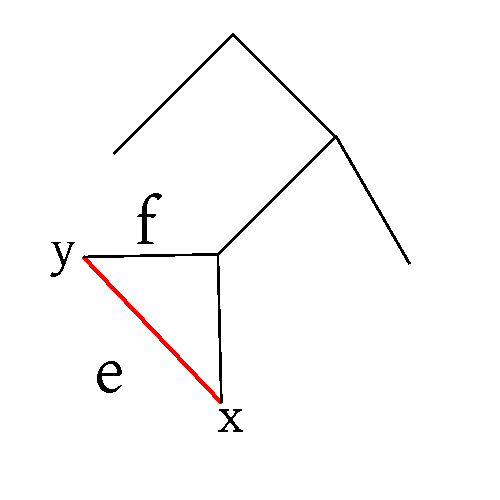
\includegraphics[width=140pt]{img/ab.pdf}
    \caption{Sketch for $a \Rightarrow b$}
  \end{center}
\end{figure}

$c(e) \geq c(f)$
for every $f$ in \gath xy in $T$, because otherwise $T - e + f$ is a spanning tree with $c(T - e  + f) = c(T) - c(e) + c(f) < c(T)$ which contradicts.

\subsubsection{$b \Rightarrow c$}
%
\begin{figure}[t]
  \begin{center}
    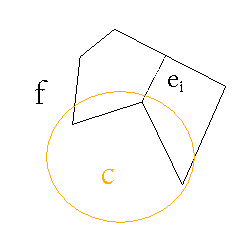
\includegraphics{img/bc.pdf}
    \caption{Sketch for $b \Rightarrow c$}
  \end{center}
\end{figure}

Show $\fall e \in E(T): c(e) \leq c(f) \fall f \in \delta(V(c))$. Every edge $e \in T$ defines an cut $\delta(V(c)) = \delta(e)$. Hence we improve the tree.

\subsubsection{$c \Rightarrow d$}
%
Show there exists some weighted order and cuts with properties like in $c$. Select a random order $\set{e_1, e_{i-1}, e_i, e_{n-1}}$. $\fall e \in \set{1, 2 \ldots, n-1}$ consider cut $\delta(c_{e_i})$. It has the desired properties.

\subsubsection{$d \Rightarrow a$}
%
Assumption $E(T) = \set{e_1, \ldots, e_{n-1}}$ is satisfied.

Let $T^*$ be an optimal spanning tree such that $i(T^*) = \min\{h \in \set{1, 2, \ldots, n-1}: e_n \notin E(T^*)\}$ is maximum.

We show $i = +\infty$ and hence $T^* \equiv T \Rightarrow T$ is optimal.
Assumption $i < +\infty$. Then $X \subset V(G)$ with $e_i \in \delta(v)$ with minimum weight with $e_j \notin \delta(X) \fall j < i$.
\[
  \exists f \neq e_i \text{ with } f \in T^* \cap \delta(X)
\] \[
  c(f) \geq c(e_i)
\] \[
  c(f) \leq c(e_i)
\] \[
  \Rightarrow c(f) = c(e_i)
\]

$T^* - f + e_i$ is an optimal spanning tree and has $i(T^* - f + e_i) > i(T^*)$. This is a contradiction.

\subsection{Kruskal's algorithm}
%
\dateref{7th of Oct 2014}

\begin{algorithm}
  \caption{Kruskal's algorithm}
  \label{kruskals-algo}
  \given{$G$ is a connected undirected graph, $c: E(G) \rightarrow \mathbb{R}$}
  \find{minimum spanning tree}
\begin{algorithmic}[1]
  \State Sort edges $c(e_1) \leq c(e_2) \leq \ldots \leq c(e_m) \qquad (m = \card{E(G)})$
  \State Set $T := (V(G), \phi)$
  \For{$i$ from $1$ to $m$}
    \If{$T \cup \set{e_i}$ is cycle-free}
      \State $E(T) = E(T) \cup \set{e_i}$
    \EndIf
  \EndFor
\end{algorithmic}
\end{algorithm}

\begin{theorem}\label{satz-2.3}
  Krukal's algorithm is correct.
\end{theorem}

From the previous theorem we can derive: $\fall e = \set{x, y} \notin E(T)$
we can say $c(f) \leq c(e) \fall f$ edges from the \gath xy in $T$.
\[
    (x, y) = e \notin E(T) \Rightarrow e_i \text{ closes cycle with } E(T) \cap \set{e_1, \ldots, e_{i-1}}
\] \[
    \Rightarrow E(x-y-\text{path} \in T) \subseteq \set{e_1, \ldots, e_{i-1}}
\] \[
    \Rightarrow \fall f \in E(x-y-\text{path}): c(f) \leq c(e_i)
\]

\textbf{Trivial implementation.}
  $\mathcal{O}(m\cdot n)$ because there are $m$ iterations and
  per iteration one check whether the current edge with the given $T$ ($\leq n$ edges)
  creates a cycle ($\mathcal{O}(n)$ with DFS).

\index{branching}
\textbf{Definition.}
  A digraph $G$ is called \emph{branching}, if it is cycle-free and
  every $v \in V(G): \operatorname{indegree}(v) \leq 1$.

\textbf{Notation.}
  $\operatorname{indegree}(v) = \operatorname{deg}^-(v)$.

\index{arborescence}
\textbf{Definition.}
  A connected branching is called \emph{arborescence}.
  The vertex $r$ with $\operatorname{deg}^-(r) = 0$ is called \emph{root}.
  An arborescence is the directed-graph equivalent of a rooted tree.

\textbf{Notation.}
  \[
    \delta(\set{v}) = \delta(v)
  \] \[
    \delta^+(v) = \set{e = (v, y) \in E(G)}
  \] \[
    \delta^-(v) = \set{e = (x, v) \in E(G)}
  \]

\begin{theorem}\label{satz-2.4}
  Let $G$ be a digraph with $n$ vertices. The following 7 statements are equivalent:
\begin{enumerate}
  \item $G$ is an arborescence with root $r$.
  \item $G$ is a branching with $n-1$ edges and $\operatorname{deg}^-(r) = 0$.
  \item $G$ has $n-1$ edges and every vertices is reachable from $r$.
  \item Every vertex is reachable from $r$ and removal of one edge destroys this property.
  \item $G$ satisfies $\delta^+(X) \neq 0 \fall X \subset V(G)$ with $r \in X$. The removal of one arbitrary edge destroys this property.
  \item $\delta^-(r) = 0$ and $\fall v \in V(G) \setminus \set{r} \exists$ one distinct directed $r-v$-path in $G$
  \item $\delta^-(r) = 0$ and $\card{\delta^-(v)} = 1 \fall v \in V(G) \setminus \set{r}$ and $G$ is cycle-free.
\end{enumerate}
\end{theorem}

\noproof{satz-2.4} It will be provided in the practicals.

\begin{theorem}\label{satz-2.5}
  Kruskal's algorithm can be implemented with time complexity $\mathcal{O}(m \log{n})$.
\end{theorem}

\begin{proof}
  The implementation keeps a branching $B$ with
  \begin{itemize}
    \item $V(B) = V(G)$
    \item connected components of $B$ vertex-correspond with the connected components of $T$
  \end{itemize}
\end{proof}

How can we create such a branching?
\begin{enumerate}
  \item At the beginning (after initialization): $B = (V(G), 0)$.
\end{enumerate}

Be aware that checking whether $\set{v, w}$ creates a cycle with $T$, consider that $w$ must be in the same connected component in $T$ (or $B$).
We can check this in $\mathcal{O}(\log{n})$.

In branching:
\begin{itemize}
  \item Let $r_v(r_w)$ be the root of $v(w)$ contained solutions of $B$.
    \[
      r_v = r_w
    \]
    The computational effort for checking is equivalent to the effort for the determination of $r_v$ and $r_w$
    which is proportional to the sum of the lengths of \gath{r_v}{v} or \gath{r_w}{w} in $B$.
\end{itemize}

\begin{hypothesis}
  In $B$ it holds that $h(r) \leq \log{n}$ for every root $r$ where $h(r)$ is the maximum length of an \gath rv in $B$.
\end{hypothesis}

\begin{figure}[ht]
  \begin{center}
    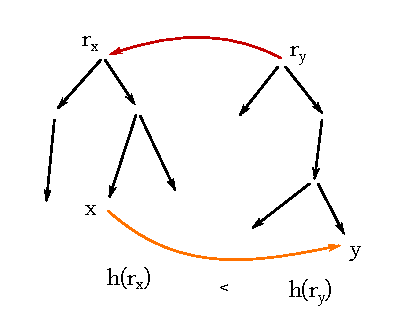
\includegraphics{img/branching_insertion.pdf}
    \caption{Branching insertion operation}
  \end{center}
\end{figure}

\begin{proof}
  Induction over number of edges in $B$.

  \textbf{Base.} For zero edges this is trivial to prove. \\
  \textbf{Step.}
    We will add a new edge $\set{x, y}$ and beforehand $h(r) \leq \log{n}$ is satisfied.
    We have to show that $h(r) \leq \log{n}$ is satisfied after the insertion of $\{x, y\}$.

    Case distinction:
    \begin{itemize}
      \item $h(r_x) = h(r_y)$. Insert $(r_x, r_y)$ or $(r_y, r_x)$
        In the figure we have to ensure $h(r_x) \leq \log{r_x} \Leftrightarrow m_x \leq 2^{h(r_x)}$.
        \[
          \hat h(r_x) = h(r_x) + 1
        \] \[
          n_{x,y} = n_x + n_y \geq 2^{h(r_x)} + 2^{h(r_y)}
        \] \[
          = 2 \cdot 2^{h(r_x)} = 2^{h(r_x) + 1}
        \] \[
          = 2^{\hat h(r_x)}
        \]
      \item $h(r_x) < h(r_y)$. Insert $(r_y, r_x)$.
        \[
          \hat h(r_y) = h(r_y)
        \] \[
          n_{xy} \geq n_y \geq 2^{h(r_y)} = 2^{\hat h(r_y)}
        \]
    \end{itemize}
\end{proof}

\subsection{Prim's algorithm}
%
\begin{algorithm}
  \caption{Prim's algorithm}
  \label{prims-algo}
  \given{$G$ is a connected undirected graph, $c: E(G) \rightarrow \mathbb{R}$}
  \find{minimum spanning tree}
\begin{algorithmic}[1]
  \State Set $T = (\set{v}, 0)$ for an arbitrary $v \in V(G)$
  \While{$V(T) \neq V(G)$}
    \State Select one edge $e \in \delta_G(V(T))$ with minimum weight
    \State $T := T + e$
  \EndWhile
\end{algorithmic}
\end{algorithm}

\begin{theorem}\label{satz-2.6}
  Prim's algorithm is correct and can be implemented with time complexity of $\mathcal{O}(n^2)$.
  Correctness follows from theorem 2.2.d ($a \Rightarrow b \Rightarrow c \Rightarrow d \Rightarrow a$):
    Spanning tree is optimal $\Leftrightarrow$ order of edges $e_1, \ldots, e_{n-1}$ such that
    $\fall i \in \set{1, 2, \ldots, n-1} \exists x_i \subset V(G)$ with $e_i \in \delta(X_i)$
    is the minimum edge in $\delta(X_i)$ and $e_j \notin \delta(X_i)$ is the cheapest edge of $\delta(X_i)$
    and $e_j \notin \delta(X_i) \fall 1 \leq j \leq i-1$. This is satisfied by construction.
\end{theorem}

The desired order (or cuts) will be created by the algorithm.

\textbf{Time complexity.} The number of iterations is the number of edges in the tree which is $n-1$.
We have to show that every iteration is completed in $\mathcal{O}(n)$ time.

Maintain a list of candidate edges: $\fall w \notin V(T)$ is the candidate edge $K(w)$ the minimum edge between $w$ and $V(T)$.
In the general case we add the minimum edge $K(w) \fall w \notin V(T)$ ($T = T + k(w)$).

\textbf{Definition.}
  $\card{V(G) \setminus V(T)} = \mathcal{O}(n)$ can be computed in $\mathcal{O}(n)$ time.

Update of candidate edges: If $v_k$ was added to $T$ in the last iteration then compare $c(v_k, w), c(k(w))$ and if $c(v_k, w) < c(k(w))$ then $k(w) = (v_k, w)$. This requires $\mathcal{O}(n)$ time.

\begin{theorem}\label{satz-2.7}
  Is Prim's algorithm implemented with Fibonacci-Heaps we can solve the MST problem in $\mathcal{O}(m + n\log{n})$ time.
  \[
    \mathcal{O}(n^2) \qquad \mathcal{O}(m + n\log{n}) \qquad m = \theta(n^2) \qquad G \text{ is dense}
  \]
\end{theorem}

A proof for Theorem~\ref{satz-2.7} is not provided.

\section{Number of spanning trees}

\dateref{9th of Oct 2014}

\begin{theorem}\label{satz-2.8}
  (Arthur Cayley)
  The complete graph $K_n$ has $n^{n-2}$ spanning trees.
\end{theorem}

\begin{proof}
(J. Pitman, Coalescent random forests, Journal of Combinatorial Theory A 85, 1999, 165--193)
Double-counting approach counting the number of labelled rooted trees (LRT). In labelled trees every edge has a label. Two LRTs are equivalent if and only if their tree structure is the same and labels are equivalent.

\begin{enumerate}
  \item Let $\tau(n)$ be the number of spanning trees in $K_n$. Every tree can have $n$ root candidates and $(n-1)!$ labels. In conclusion we can create $n \cdot (n-1)! \cdot \tau(n)$ LRTs with $n$ vertices.
  \item Insert edges successively such that adding $n-1$ vertices creates a LRT. For one edge we have \dots
    \[
      2 \cdot \frac{n(n-1)}{2} = n(n-1) \text{ possibilities}
    \]
    We added $k$ edges ($k < n -1$). Followingly the graph has $n-k$ connected components with $n_1, n_2, \ldots, n_{m-k}$ vertices each. Every connected component is a LRT. If the $k+1$-th edge to be added starts at component $1$, then this edge must have the root as source. This edge can have every other vertex as destination. There are $n-n_1$ possible such edges. In total we start with an arbitrary component and get:
    \[
      (n - n_1) + (n - n_2) + \ldots + (n - n_{n-k}) = n (n-k) - n
    \]
    This is the number of possilities for edge $k+1$.
    In total for all $n-1$ edges to add:
    \[
      \prod_{k=0}^{n-2} (n \cdot (n-k) - n) = \prod_{k=0}^{n-2} n (\underbrace{n - k - 1}_{1 \leq t \leq n-1}) = n^{n-1} (n - 1)
    \]
    It holds:
    \[
      n (n-1) ! \delta(n) = n^{n-1} (n-1)! \Rightarrow \delta(n) = n^{n-2}
    \]
\end{enumerate}
\end{proof}

\subsection{Minimum Weight Arborescence Problem (MWA)}
%
\given{Digraph $G = (V, E), c: E(b) \rightarrow \mathbb{R}$}
\find{Spanning arborescence with minimum weight or claim $\nexists$ spanning arborescence in $G$}
%
\subsection{Minimum Weighted Rooted Arborescence Problem (MWRA)}
%
\given{Digraph $G = (V, E), r \in V(G), c: E(G) \rightarrow \mathbb{R}$}
\find{Spanning arborescence with root $r$ and with minimum weight in $G$ or claim $\nexists$ spanning tree with root $r$ in $G$}
%
\subsection{Maximum Weighted Branching Problem (MWB)}
%
\given{Digraph $G = (V, E), c: E(G) \rightarrow \mathbb{R}$}
\find{Branching $B$ with maximum weight}
%
\subsection{Equivalence of MWA, MWRA and MWB}
%
\begin{hypothesis}
  The three problems MWA, MWRA and MWB are equivalent.
\end{hypothesis}

Partially the proof is given in the practicals.

\begin{proof}
We assume without loss of generality that $c(e) \geq 0 \fall e \in E(G)$ because negative edges cannot occur in a maximum branching.
\[
    \deg^-(v) \leq 1 \fall v \in V(G)
\]

\textbf{Greedy approach:} $\fall v \in V(G)$ select one $e_v \in \argmax\{c(e): e = (x, v) \in E(G)\}$ let $B := \set{e_v: v \in V(G)}$.

If $B_0$ is cycle-free: $B_0$ is branching with maximum weight. Otherwise cycles have to be avoided / destroyed.

\begin{theorem}\label{lemma-2.10}
  Let $B_0$ be a subgraph of $G$ with maximum weight and $\deg^-_{B_0}(v) \leq 1 \fall v \in V(G)$.
  Then $\exists$ an optimal branching $B \in G$ with properties $\fall$ cycle $C \in B_0: \card{E(C) \setminus E(B)} = 1$.
\end{theorem}

\begin{proof}
\textbf{Assumption.}
  Such an optimal branching $B$ does not exist.

Let $B$ be a maximum branching in $G$ with maximum number of common edges with $B_0$. Let $C$ be a cycle in $B_0$ with $\card{E(C) \setminus E(B)} \geq 2$.
\[
  E(C) \setminus E(B) = \set{(a_1, b_1), (a_2, b_2), \ldots, (a_k, b_k)}
\]
in order they appear inside the cycle.

\begin{hypothesis}
  \[
    \fall 1 \leq i \leq k \exists b_i-b_{i-1}-\text{path in } B (b_0 \equiv b_k)
  \]
\end{hypothesis}

\begin{figure}[ht]
  \begin{center}
    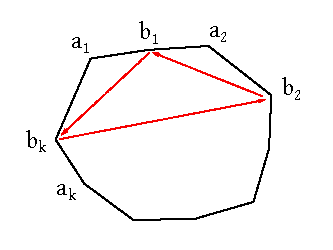
\includegraphics{img/red_cycle.pdf}
    \caption{Red cycle}
  \end{center}
\end{figure}

The existence of a red cycle in $B$ shows a contradiction.
\end{proof}

Consider a fixed $i \in \set{1, 2, \ldots, k}$.
Let $B_i'$ be a subgraph of $G$ with $V(B_i') = V(G)$ and $E(B_i') = \set{(x, y) \in B: y \neq b_i} \cup \set{(a_i, b_i)}$. If so, then $c(B_i') \geq c(B)$ and thus $B_i'$ would be an optimal branch with one common edge $(a, b)$ more in $B_0$. This is a contradiction.

$B_1'$ is no branching. So there is a cycle in $B_i'$, which contains $(a_i, b_i)$. So a \gath{b_i}{a_i} in $B_i'$ is exists in $B$.
\end{proof}

This \gath{b_i}{a_i} does not exist in $C$. Otherwise he would be forced to use an edge $(a_i, b_i)$ which he is not allowed to do so, because $(a_i, b_i) \nexists B$.

Let $e = (x, y)$ be the last edge of the \gath{b_i}{a_i} which is outside of the cycle. $y = b_j$ must hold because otherwise there are two discharging edges in $B$, which is a contradiction.

\subsection[Edmonds' branching algorithm]{Edmonds' branching algorithm (1967)}
%
% TODO: terrible to understand. refactor the algorithm
\begin{algorithm}
  \caption{Edmonds' branching algorithm (book: page~153)}
  \label{edmonds-branching-algo}
  \given{Digraph $G$, weights $c: E(G) \rightarrow \mathbb{R}_+$}
  \find{A branching $B$ of $G$ with maximum weight}
  \textbf{Remark:}
    $\alpha(e, C)$ is the edge $(u, v)$ inside $C$, which shares $v$ as destination with $e$ but not $u$.
    $\psi_i(e)$ is the edge $e$ in the iteration $i$ of the algorithm. \par
\begin{algorithmic}[1]
  \State Set $i := 0, G_0 := G, c_0 := c$.
  \State Let $B_i$ be a subgraph of $G_i$ with maximum weight and $\card{\delta_{B_i}^-(v)} \leq 1$ for all $v \in V(B_i)$\label{eba-step-2}
  \If{$B_i$ is cycle-free}
    \State $B := B_i$
    \Goto{eba-step-5}
  \EndIf
  \State Let $\mathcal{C}$ be the set of cycles in $B_i$. Select one $C \in \mathcal{C}$.
  \State Let $V(G_{i+1}) := \mathcal{C} \cup (V(G_i) \setminus \bigcup_{C \in \mathcal{C}} V(C))$.
  \For{$e = (v, w) \in E(G_i)$} % TODO: verify correctness
    \State $e' = (v', w') \in E(G_{i+1})$
    \State $\Phi_{i+1}(e') := e$ where
    \Statex
      $v' = C$ if $v \in V(C)$ for $C \in \mathcal{C}$ and
      $v' = v$ if $v \notin \bigcup_{C \in \mathcal{C}} V(C)$ and
    \Statex
      $w' = C$ if $w \in V(C)$ for $C \in \mathcal{C}$ and
      $w' = w$ if $w \notin \bigcup_{C \in \mathcal{C}} V(C)$.
  \EndFor
  \State Let $E(G_{i+1}) := \set{e' = (v', w'): e \in E(G_i), v' \neq w'}$ \Comment{(parallel edges might occur)}
  \For{$e = (v, w) \in E(G_i)$ with $e' = (v', w') \in E(G_{i+1})$} % TODO: verify correctness
    \State $c_{i+1}(e') := c_i(e) \text{ if } w' \notin \mathcal{C}$
    \State $c_{i+1}(e') := c_i(e) - c_i(\alpha(e, C)) + c_i(e_C)$
    \Statex
      if $w' \in C \in \mathcal{C}$ where $\alpha(e, C) \in \delta^-_C(w)$ and $e_C$ is the cheapest edge of $C$.
  \EndFor
  \State Set $i := i + 1$
  \Goto{eba-step-2}
  \While{$i > 0$ \label{eba-step-5}}
    \State $B' := (V(G_{i-1}), \set{\Phi_i(e): e \in E(B)})$
    \For{every cycle $C$ of $B_{i-1}$}
      \If{some edge $e \in \delta_{B'}^-(V(C))$ exists}
        \State $E(B') := E(B') \cup (E(C) \setminus \set{\alpha(e, C)})$ \Comment{Delete $\alpha(e,C)$}
      \Else
        \State $E(B') := E(B') \cup (E(C) \setminus \set{e_C})$ \Comment{Delete cheapest edge in cycle}
      \EndIf
    \EndFor
    \State $B := B'$
    \State $i := i - 1$
  \EndWhile
\end{algorithmic}
\end{algorithm}

\index{contraction}
A \emph{contraction} is the process to replace several vertices $C$ with a single
new vertex $v'$. Handling edges must be defined explicitly, but in general it works
something like $G' = (V, \set{(v, v') \,|\, (v, u) \in E \land u \in C}
\cup \set{(v', v) \,|, (v, u) \in E \land v \in C})$.

\begin{theorem}\label{satz-2.11}
  Edmonds' Branching Algorithm is correct and computes the branching of
  maximum weight in $\mathcal{O}(m\cdot n)$.
\end{theorem}

\begin{proof}
The algorithm constructs a sequence of graphs $G_0 = G, G_1, \ldots, G_k$ are edge-weight-free $c_0 = c, c_1, \ldots, c_k$ until the ``greedy solution'' in the current $G_k$ is also a branching ($B_k$). Then the algorithm transform this $B_k$ into a branching $B_{k+1}$ in $G_k$ successively until $G_0$. It suffices to show that the transformation of a branching $B_i$ into $B_{i+1}$ provides a branching. With induction it immediately follows that the $B_0$ branching in $G_0 = G$.

Let $B_i$ be a branching in $G$. We show that the algorithm's $B^*_{i-1}$ is an optimal branching in $G_i$ with $\card{E(C) \setminus E(B^*_{i-1})}$.

The number of cycles $C$ in $B_{i-1} = 1$ ($B_{i-1}$ exists according to our previous theorem).

We derive $B^*_i$ from $B^*_{i-1}$ by the constructed cycle of $B_{i-1}$. Then $B^*_i$ is a branching in $G_i$.

\[
  c_{i-1}(B_{i-1}^*) = c_i(B_i^*) + \sum_{C' \text{cycle} \in B_{i-1}}(c_{i-1}(C') - c_{i-1}(e(C')))
\] \[
  c_{i-1}(B_i) \geq c_i(B^*_i)
\] \[
  c_{i-1}(B_{i-1}^*) \leq c_i(B_i) + \sum_{C' \text{cycle} \in B_{i-1}} \left[ c_{i-1}(C') - c(e(C')) \right]
\] \[
  = c_{i-1}(B_{i-1})
\]
so $B_i$ is an optimal branching of $G_i$ according to the induction hypothesis.

\textbf{Runtime analysis.}
  $n$ iterations, $\mathcal{O}(m)$ time per iteration
\end{proof}

\section{Shortest path problems in graphs}
%
\dateref{13th of Oct 2014}

\given{$G = (V, E)$ is a digraph.}

A sequence of vertices $v_1, v_2, \ldots, v_k$ is called \emph{edge sequence} if $(v_i, v_{i+1}) \in E(G) \fall 1 \leq i \leq k-1$. A sequence of vertices $v_1, \ldots, v_k$ such that $\fall e \in E(G)$ there is at most one index $1 \leq i \leq k-1$ with $e = (V_i, V_{i+1})$ is called a \emph{walk}. A walk which does not use any vertex twice is called \emph{path}.

We distinguish between inner vertices and end vertices. A path with end vertices $u$ and $v$ is a \gath uv. Let $P = (v_1, \ldots, v_k)$ a \gath{v_1}{v_2} and $1 \leq i < j \leq k$. Then compute only $(v_i, v_{i+1}, \ldots, v_j)$ as $P_{[v_i, v_j]}$.

A \emph{cycle} (a path with the same start and end vertex) is a \emph{closed path}. Let $s, t \in V(G)$ then
\[
  d(s, t) := \left\{\begin{array}{lc}
    \text{length (number of edges) of the shortest \gath st in $G$} & \\
    +\infty & \nexists s-t-\text{path}
  \end{array}\right.
\]

If $c \in E(G) \rightarrow \mathbb{R}$
\[
    d^G(s, t) = \left\{\begin{array}{lc}
      \sum_{e \in P} c(e) & \text{where P is the shortest path in G with c} \\
      +\infty & \nexists s-t-\text{path}
    \end{array}\right.
\]

\subsection{Single source shortest path problems (SSSP)}
%
\given{$G = (V, E)$ is a digraph, $c: E(G) \rightarrow \mathbb{R}, s \in V(G)$}
\find{$\fall v \in V(G)$ find a shortest \gath st in $G$}

Consider a digraph $G$ where $c(e) = -1 \fall e \in E(G)$ and $s,t \in V(G)$. The shortest path is to visit all edges infinitely. A \gath st has at maximum $n-2$ vertices
\[
    \geq d^G(s, t) \geq -(n - 1)
\] \[
    d^G(s, t) = -(n - 1) \Leftrightarrow \exists \text{Hamiltonian $s-t$-path in $G$}
\]

Detection of Hamiltonian paths is a NP-complete problem.

\textbf{Definition.}
  A weighting $w$ in a graph $D$ is called \emph{conservative}, if the sum of weights in every cycle of $D$ is non-negative. In other words:
  \begin{itemize}
    \item $\nexists$ negative cycles in $G$.
    \item Let $K$ be the set of cycles in a graph $G$. For every cycle $C \in K$, $w(C) \geq 0$ holds with $w(C) := \sum_{e \in E(C)} c(e)$.
    \item In case of digraphs, directed cycles have to be considered.
  \end{itemize}

\textbf{Remark.}
  Analogous problem in undirected graphs are in general more difficult that in digraphs.

If $c(e) \geq 0 \fall e \in E(G)$ the graph can be transformed into a digraph.

\begin{theorem}\label{proposition-3.1}
Let $G$ be a digraph with conservative weights. $c: E(G) \rightarrow \mathbb{R}$. Let $s, w \in V(G)$ and $k \in \mathbb{N}$. Let $P$ be the shortest among all \gath swes with at most $k$ edges. Let $e = (v, w)$ be the last edge of $P$. Then $P_{[s, w]}$ is the shortest \gath sv with at most $(k-1)$ edges.
\end{theorem}

\begin{proof}
We assume $\exists$ \gath sv $Q$ with $c(Q) < c(P_{[s,v]})$. Case distinction:
\begin{enumerate}
  \item $w \notin V(Q)$. Consider \gath sw $P_1$ as chain of $Q$ with $(v, w)$. Then
    \[
      c(P_1) = c(Q) + c(v, w) < c(P_{[s,v]}) + c(v,w) = c(P)
    \]
    This is a contradiction.
  \item
    \[
      c(Q_{[s,w]}) = c(Q) - c(Q_{[w,v]})
        = \underbrace{c(Q)}_{c(P_{[s,v]})} + c(v,w) - [c(Q_{w,v}) + c(v,w)]
    \] \[
        < \underbrace{c(P)}_{P_{[s,v]}(v,w)}
          - \underbrace{\left(c(Q_{[w,v]}) + c(v,w)\right)}_{\text{cycle }K}
        \leq c(Pc)
    \]
    We select $P$ because $Q_{[s,w]}$ is shorter than $P$ and has at most $k-1$ edges as part of a \gath sv $Q$. This is also a contradiction.
\end{enumerate}
\end{proof}

In the following we assume $c(e) \geq 0 \fall e \in E(G)$.

\subsection{Dijkstra's algorithm for SSSP}
%
\begin{algorithm}
  \caption{Dijkstra's algorithm}
  \label{dijkstras-algo}
  \given{$G = (V, E)$ is a digraph. $c: E(G) \rightarrow \mathbb{R}^+, s \in V(G)$}
  \find{A shortest path of $s$ to $v, \fall v \in V(G)$. Let $l(v)$ be the length of a shortest path $s-v$ in $G$ and $p(v)$, such that $p(v)$ is the predecessor of $v$ of the shortest \gath sv in $G$ provided by the algorithm $\fall v \in V(G)$. If $v$ is not reachable from $j$, then $l(v) = +\infty$ and $p(v)$ is not defined.}
\begin{algorithmic}[1]
  \State Let $l(s) = 0$, $l(v) = \infty \fall v \in V(G) \setminus \set{s}$, $p(s) = 0$, $R = \set{}$
  \State Find $v \in V(G) \setminus R$ with $l(r) = \min\set{e(x) : x \in V(G) \setminus R}$ \label{dijkstra-redo}
  \State Let $R = R \cup \set{v}$
  \For{$w \in V(G) \setminus R$ with $(v, w) \in E(G)$}
    \If{$l(w) > l(v) + c(v, w)$}
      \State $\set{l(w) := l(v) + c(v, w); p(w) = v}$
    \EndIf
  \EndFor
  \If{$R \neq V(G)$}
    \Goto{dijkstra-redo}
  \EndIf
\end{algorithmic}
\end{algorithm}

\begin{theorem}\label{satz-3.2}
  Dijkstra's algorithm is correct and can be implemented in $\mathcal{O}(n^2)$.
\end{theorem}

\begin{proof}
  The following statements are invariants of the algorithms:
  \begin{enumerate}
    \item $\fall v \in V(G) \setminus \set{v}$ with $l(v) < +\infty$ results in $p(v) \in R$, $e(p(v)) + c(p(v), v) = l(v)$ and $v, p(v), p(p(v)), \ldots$ contains $1$.
    \item $\fall v \in R$ it holds that $l(v) = \operatorname{dist}^{(G,c)}(s, v)$.
  \end{enumerate}
  Why?
  \begin{itemize}
    \item
      After step 1 of the algorithm, both invariants are inherently satisfied.
      In step 4 we update $l(w)$ and $p(v) = v$ for some $v \in R$ and also $l(u) = l(v) - c(v, w) = l(p(w)) + c(p(w), w)$. $v, p(v), \ldots$ contains $s$ because at the beginning $s$ was the only vertex with $e(\dots) < \infty$.
    \item
      $s \in R$ holds $c(s) = 0 = C(\text{shortest path})$.
      Induction over $\card{R}$
      \begin{description}
        \item[induction base] $R = \set{s}$ (trivial).
        \item[induction step] Statement is satisfied until the execution of step 3. We have to show that the statement holds after step 3. We assume that this statement is not satisfied. Then for $v$ in step 3 there is some \gath sv $P$ in $G$ with $c(P) < l(v)$. Let $y$ be the first vertex in $P$ which is part of $(V(G) \setminus R) \cup \set{v}$ and $x$ is the predecessor of $y$ in $P$.
        Then it holds $x \in R$ in $P$. From the induction assumption if follows that $\operatorname{dest}^{G,C}(s,x) = l(x)$.
        \[
          l(y) \leq l(x) + c(x, y) = \operatorname{dest}^{G,C}(s, x) + c(x,y) \leq c(P_{[s,y]}) \leq c(P) < l(v)
        \]
        This is a contradiction.
        Directly after $R = R \cup \set{x}$ it holds that after execution of step 4 of the algorithm $l(y) = l(x) + c(x, y)$. Followingly $l(x)$ does not change any more because $x \in R$ and $l(y)$ can only be reduced.
      \end{description}
  \end{itemize}
\end{proof}

\subsubsection{Analysis}
%
$\mathcal{O}(n^2)$ because we have $n$ iterations and an effort of $\mathcal{O}(n)$ per iteration.

\begin{theorem}\label{satz-3.3}
  (Fredman and Tarjan, 1987)
  A Fibonacci-Heap implementation of Dijkstra's algorithm runs in $\mathcal{O}(m + n\log{n})$ time.
\end{theorem}

\noproof{satz-3.3}

For planar graphs Dijkstra's algorithm can be implemented with $\mathcal{O}(n)$ time (Henzinger, 1997). For weights of integers $\geq 0$ it can be implemented in $\mathcal{O}(n)$ (Thomp, 1999).

\subsection{Moore-Bellman-Ford algorithm}
%
\begin{algorithm}
  \caption{Moore-Bellman-Ford algorithm}
  \label{mbf-algo}
  \given{A digraph $G=(V, E)$, conservative $c: E(G) \rightarrow \mathbb{R}$, $s \in V(G)$}
  \find{$l(v), p(v)$ like Dijkstra's algorithm $\fall v \in V(G)$}
\begin{algorithmic}[1]
  \State $l(s) := 0, \quad l(v) := \infty \fall v \in V(G) \setminus \set{s} \quad p(s) = 0$
  \For{$i = 1$ to $n-1$}
    \For{$(u, w) \in E(G)$}
      \If{$l(w) > l(u) + c(u, w)$}
        \State $l(w) := l(u) + c(u, w)$
        \State $p(w) := u$
      \EndIf
    \EndFor
  \EndFor
\end{algorithmic}
\end{algorithm}

\subsubsection{Analysis}

\begin{theorem}\label{satz-3.4}
  The Moore-Bellman-Ford algorithm is correct and has runtime $\mathcal{O}(nm)$.
\end{theorem}

We have $\mathcal{O}(n)$ iterations and need $\mathcal{O}(m)$ time per iteration.

\dateref{14th of Oct 2014}

\begin{proof}
  Let $R := \set{v \in V(G): l(v) < +\infty}$ and $F := \set{(x, y) \in E(G): x = p(y)}$.
  The following statements are invariants of the algorithm (even for non-conversative weights):
  \begin{enumerate}
    \item $l(y) \geq l(x) + c(x, y) \fall (x, y) \in F$
    \item If $F$ contains a cycle $K$, then $K$ has a negative weight $c(K) < 0$.
  \end{enumerate}

  \textbf{Assumption.}
    A cycle $K$ in $F$ is created by insertion of edge $(x, y)$. At this point in time $p(y) = x$ will be set in the second step. Before $l(y) = l(x) + c(x, y)$ was set because previously it holds that $l(y) > l(x) + c(x, y) \fall (v, w) \in F$ and $l(w) \geq l(v) + c(v, w)$.
  \begin{figure}[!ht]
    \begin{center}
      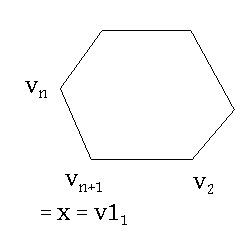
\includegraphics{img/cycle.pdf}
      \caption{Cycle creation by edge insertion}
    \end{center}
  \end{figure}
  \[
    \sum_{i=1}^{n} l(v_i) = l(v_i) + \sum_{i=1, i\neq2}^n l(v_i) + c(v_1, v_2) = \sum_{i=1,i\neq2}^n [l(v_i) + c(v_i, v_{i+1})]
  \] \[
    \Leftrightarrow \sum_{i=1}^n l(v_i) > \sum_{i=1}^n l(v_i) + \sum_{i=1}^n c(v_i, v_{i+1})
  \] \[
    \Leftrightarrow C(k) = \sum_{i=1}^n c(v_i, v_{i+1}) < 0
  \]
  Hence if $c$ is conservative, then $F$ is cycle-free.

  \[
    x \in R \Rightarrow l(x) < \infty \Rightarrow l(p(x)) < \infty \Rightarrow p(x) \in R
  \] \[
    \Rightarrow p(p(x) \in R) \text{ until s}
  \]
  Followingly $\fall x \in R \exists$ some \gath sx in $(R, F)$ and $F$ is cycle-free. We conclude that $(R, F)$ is some arborescence  with root $s$.

  \begin{hypothesis} % no label
    After $k$ iterations the length (sum of weights) of the shortest \gath sx with at most $k$ edges is at least $l(x) \fall x \in R$.
  \end{hypothesis}

  We prove it by induction over $k$. Let $P_{s,x}$ be the \gath sx in $(R, F)$.
  \[
    l(x) \geq^a l(p(x)) + c(p(x), x) \geq^a l(p(p(x))) + c(p(p(x)), p(x)) + c(p(x), x)
  \] \[
    \geq^a \ldots \geq^a l(s) + \sum_{e \in P_{s,x}} c(e) = c(P_{s,x}) \fall x \in R
  \]

  \begin{description}
    \item[Induction base.]
      For $k=1$ all edges start at the same vertex. \\
      \[
        l(v) = l(s) + c(s, v) \qquad \text{ thus } l(v) = c(s, v) \fall v \text{ with } l(v) < \infty
      \]

    \item[Induction step.]
    \textbf{Assumption.}
      Assumption holds after $k$ iterations. \\
    \textbf{Show.}
      Assumption holds after $k+1$ iterations.

    Let $P$ be a shortest \gath sv with at most $k+1$ edges. Let $(w, x)$ be the last edge in $P$. From the proposition~\ref{proposition-3.1} (every subpath of the shortest path is also a shortest path) it follows that $P_{[s,w]}$ is the shortest \gath sw with at most $k$ edges.
    \[
      l(w) \leq c(P_{[s,w]})
    \]
    Iteration $k+1$ will also analyze $(w, x)$. Followingly it must hold that
    \[
      l(x) \leq l(w) + c(w, x) \leq c(P_{[s,w]}) + c(w, x) = c(P)
    \]
    From the proofs of both previous assumptions we conclude that at termination it holds that
    \[
      l(x) = \text{ length of the shortest \gath sx with at most } (n-1) \text{ edges}
    \] \[
      = \text{ length of the shortest s-x-path (conservative!)}
    \]

    \textbf{Remark.}
      $(R, F)$ is the so-called ``shortest paths tree''.
  \end{description}
\end{proof}

\section{Potential}

\textbf{Definition.} Let $G = (V, W)$ be a digraph with $c: E \rightarrow \mathbb{R}$

A mapping $\pi: V(G) \rightarrow \mathbb{R}$ with $c(u, v) + \pi(u) - \pi(v) \geq 0 \fall (u, v) \in E(G)$ is called ``potential''.

\begin{theorem}\label{satz-3.5}
Let $G$ be a digraph with $c: E(G) \rightarrow \mathbb{R}$. A potential of $(G, c)$ exists iff $c$ is conservative.
\end{theorem}

\begin{proof}
\[
  \Rightarrow \exists \text{ potential } \pi \Rightarrow c \text{ is conservative}
\]
Let $k$ be a cycle
\[
  c(k) = \sum_{e \in E(k)} c(e) = \sum_{i=1}^l c(v_i, v_{i+1})
    = \sum_{i=1}^l \left[c(v, v_{i+1}) + \pi(v_i) - \pi(v_{i+1}) \right]
    \geq 0
\] \[
  \Leftrightarrow \text{ c is conservative } \Rightarrow \exists \text{ potential } \pi
\]
Apply Moore-Bellman-Ford algorithm to $(\overline{G}, \overline{i})$ where $V(\overline{G}) = V(G) \dotcup \set{s}$ and $E(\overline{G}) = E(G) \cup \set{(s, v): \fall v \in V(G)}$.
\[
  \overline{c}(e) = \left\{\begin{array}{cl}
    c(e) & e \in E(G) \\
    0 & e = (s, v) \fall v \in V(G)
  \end{array}\right\}
\]

Let $l(v) \fall v \in V(\overline{G})$ be the output.

\[
  \overline{c}(v, w) + l(v) - l(w) \geq 0
\] \[
  l(w) \leq l(v) + c(v, w)
\]
\end{proof}

\textbf{Remark.}
  The Moore-Bellman-Ford algorithm (as shown above) can be used to determine whether $c$ is conservative and possibly to compute a potential.

\begin{theorem}\label{korollar-3.5}
  Let $G = (V, E)$ be a digraph with $c: E(G) \rightarrow \mathbb{R}$. The Moore-Bellman-Ford algorithm can either determine a desired potential or find a negative cycle in $\mathcal{O}(m\cdot n)$ .
\end{theorem}

\begin{proof}
We apply Moore-Bellman-Ford algorithm to $(\overline{G}, \overline{i})$ as shown above and retrieve $l(v) \fall v \in V(G)$.

If $l$ is a potential, we are done.

Otherwise $\exists (u, w) \in E(G)$ with $c(u, w) + l(u) < l(w) \Rightarrow l(u)$ was changed in the last iterations $\Rightarrow$ $l(p(u))$ was changed in the last 2 iterations $\Rightarrow$ $l(p(p(u)))$ was changed in the last 3 iterations. It holds that the length $l(\ldots)$ of each of these vertices was changed while the algorithm was running.

\[
  w, u, p(u), p(p(u)), p(p(p(u))), \ldots
\]

Because $e(s)$ was not changed, $\set{w, n, p(u), \ldots, p(\ldots p(u) \ldots)}$ must contain a cycle. $K$ in $F$ $\Rightarrow$ $c(k) < 0$ from invariant of $b$ of the previous proof 3.3.
\end{proof}

\section{All Pairs Shortest Paths Problem}
%
\subsection{All pairs shortest paths problems (APSP)}
%
\given{$G = (V, E)$ is a digraph. Weights $c: E(G) \rightarrow \mathbb{R}$ are conservative}
\find{Find numbers $l_{s,t}$ and vertices $p_{s,t} \fall s, t \in V(G)$ such that $l_{s,t}$ is the length of a shortest \gath st in $G$ and $(p_{s,t}, t)$ is the last edge of the shortest path.}

This is solvable with $n$ repetitions of the Moore-Bellman-Ford algorithm for each vertex: $\mathcal{O}(n^2 \cdot m)$ runtime or find potential $\pi$ with Moore-Bellman-Ford algorithm
\[
  \overline{c}(u,v) := c(u,v) + \pi(u) - \pi(v) \geq 0 \fall (u, v) \in E(G)
\]

For every \gath sx $P$ in $G$ it holds that
\[
  \overline{c}(P)
    = \sum_{i=1}^{l-1} \overline{c}(v_i, v_{i+1})
    = \sum_{i=1}^{l-1} [c(v_i, v_{i+1}) + \pi(v_i) - \pi(v_{i+1})]
\] \[
  = \sum_{i=1}^{l-1} c(v_i, v_{i+1}) + (\pi(v_1) - \pi(v_2) + \pi(v_3) + \ldots + \pi(v_{l-1} - \pi(v_l)))
\] \[
  = c(P) = \pi(v_i) - \pi(v_i) = c(P) + \pi(s) - \pi(v)
\] \[
  \min{C(P)} = \min_{P: \text{\gath sx}} \left[E(P) - \pi(s) + \pi(x)\right]
\] \[
  = \min_{P: \text{\gath sx}} \overline{C}(P) + \pi(x) - \pi(s)
\]

Apply Dijkstra's algorithm with $(G, \overline{c})$ for every vertex: $\mathcal{O}((m + n \log{n}) \cdot n)$ (best known complexity).

\subsection{Floyd-Warshall algorithm}
%
\begin{algorithm}
  \caption{Floyd-Warshall algorithm}
  \label{fw-algo}
  \given{$G = (V, E)$ is a digraph, $c: E(G) \rightarrow \mathbb{R}$ is conservative, $n = \card{V(G)}$}
  \find{Matrices $(l_{i,j})_{1 \leq i,j \leq n}$ and $(p_{i,j})_{1 \leq i,j \leq n}$ where $l_{i,j}$ and $p_{i,j}$}
\begin{algorithmic}[1]
  \State Let $l_{i,j} := c_{i,j} \fall (i,j) \in E(G)$
  \State $l_{i,j} := +\infty \fall (i,j) \in (V(G) \times V(G)) \setminus E(G)$ with $i \neq j$
  \State $l_{i,i} = 0 \fall i \in V(G)$
  \State $p_{i,j} := i \fall (i,j) \in V(G)$
  \For{$j=1$ to $n$}
    \For{$i=1$ to $n$}
      \If{$i \neq j$}
        \For{$k = 1$ to $n$}
          \If{$k \neq i \land k\neq j$}
            \If{$(l_{i,k} > l_{i,j} + l_{j,k})$}
              \State $l_{i,k} := l_{i,j} + l_{j,k}$
              \State $p_{i,k} := p_{j,k}$
            \EndIf
          \EndIf
        \EndFor
      \EndIf
    \EndFor
  \EndFor
\end{algorithmic}
\end{algorithm}




\begin{theorem}\label{satz-3.6}
  The Floyd-Warshall algorithm works correctly and has a runtime of $\mathcal{O}(n^3)$
\end{theorem}

\begin{proof}
Proving $\mathcal{O}(n^3)$ is trivial.

After execution of the most-outer loop $j$ it holds that $\fall i,k: l_{i,k}$ is the length of the shortest \gath ik whose inner vertices are from $\set{1, 2, \ldots, j_0}$ and where $(p_{i,k}, k)$ is the last edge.

Induction over $j_0$.

\begin{description}
  \item[Induction base.] $j_0 = 0$ means considering only paths without inner vertices
  \item[Induction step.] \hfill{} \\
    \textbf{Assumption.} Hypothesis holds for $j_0 \in \set{1, 2, \ldots, n-1}$ \\
    \textbf{Show.} Hypothesis holds for $j_0 + 1$.
    Execute outer loop with $j = j_0 + 1$

    \[
      l_{i,k} > l_{i,j_0+1} + l_{j_0+1,k} \Rightarrow
        l_{i,k} = l_{i,j_0+1} + l_{j_0+1,k}, P_{i,k} = P_{j_0+1,k}
    \]
\end{description}

If $P_{i,j_0+1}$ and $P_{j_0+1,k}$ are vertex-disjoint the assumption holds. But $P_{i,j_0+1}$ and $P_{j_0+1,k}$ can only be vertex-disjoint otherwise we will get a contradiction.

\textbf{Assumption.}
 $P$ and $Q$ are not vertex-disjoint.

Remove the maximum (= inclusive maximal) closed walk from $P \cup Q$. This walk has weight $\geq 0$ (as union of cycles with $c$ are conservative). Maintain a \gath ik $R$ with inner vertices from $\set{1, 2, \ldots, j_0}$ and it holds that
\[
  C(R) + C(\text{closed walk}) = l_{i,j_0+1} + l_{j_0+1,k}
    \Rightarrow C(R) \leq l_{i,j_0+1} + l_{j_0+1,k} < l_{i,k}
\]
\end{proof}

\section{Cycles with minimum mean edge weight}
%
\dateref{21st of Oct 2014}
%
\subsection{Minimum mean-cycle problem (MMC)}
%
\given{Digraph $G_i \in t(G) \rightarrow \mathbb{R}$.}
\find{Cycle $k$ with mean edge weight minimizing}
\[
  \frac{c(E(k))}{|E(k)|} \text{ or decide ``A is acyclic''}
\]

\text{Remark.} $G$ is strongly connected $\Leftrightarrow$
\[
  \fall u, v \in V(G) \quad u \neq v
\] \[
  \exists \text{directed \gath uv and } \exists \text{ directed \gath uv}
\]

Strongly connected components can be computed in $\mathcal{O}(n + m)$ with any searching algorithm in $G$. Without loss of generality: $G$ is strongly connected, otherwise solve MMC in every strongly connected component.

Let $s$ be a vertex in $G$ such that $\exists$ \gath sv $\fall v \in V(G)$.

\begin{theorem}[Karp 1978]
  \label{satz-3.10}
  Let $G$ be a digraph with $c: E(G) \rightarrow \mathbb{R}$. Let $s \in V(G)$ such that $\fall v \in V(G) \setminus \set{s} \exists$ directed \gath sv in $G$.
  \[
    \fall x \in V(G) \fall K \in \mathbb{Z}_+:
  \] \[
    F_K(x) := \min\set{
      \sum_{i=1}^k c(v_{i-1}, v_i):
        v_0 = s, v_k = x, (v_{i-1}, v_i) \in E(G),
        \fall 1 \leq i \leq k
    }
  \]

  If there is no sequence of edges of length $k$ from $s$ to $x$, then $F_K(x) = \infty$.
  Set $\mu(G, c)$ be the minimum mean edge weight of a cycle in $(G, i)$ and $\mu(G, c) = \infty$ if $G$ is acyclic. Then it holds that
  \[
    \mu(G, c) = \min_{x \in V(G)} \max_{0 \leq k \leq n-1} \frac{F_n(x) - F_k(x)}{n-k}
  \]
\end{theorem}

\begin{proof}
\begin{enumerate}
  \item If $G$ is acyclic, $\mu(G, c) = \infty$. \\
    \begin{hypothesis}
      \[ \fall x \in V(G): \max_{0 \leq k \leq n-1} \frac{F_n(x) - F_k(v)}{n-k} = \infty \]
    \end{hypothesis}
    \textbf{Proof by contradiction.}
    \[
      \exists x \in V(G) \text{ with } \max_{0 \leq k \leq n-1} \frac{F_n(x) - F_k(x)}{n-k} < \infty
    \] \[
      \Leftrightarrow F_n(x) \text{ is finite}
    \] \[
      \Rightarrow \text{ edge repetition in order defined by } F_n(x)
    \]
    This constitutes a cycle and we have a contradiction.

  \item $G$ is cyclic.
    \begin{enumerate}
      \item $\mu(G, c) = 0 \Rightarrow$ $G$ does not have negative cycles. So $c$ is conservative.
        \[
          \Rightarrow F_n(x) \geq \operatorname{dist}_{(G,c)} (s, x) = \min_{0 \leq k \leq n-1} F_k(x) = F_{k_0}(x)
        \] \[
          \Rightarrow \max_{0 \leq k \leq n-1} \frac{F_n(x) - F_k(x)}{n-k} \geq 0 \fall x \in V(G)
        \]
        We show $\exists x \in V(G)$ with \[
          \max_{0 \leq k \leq n-1} \frac{F_n(x) - F_k(x)}{n-k} = 0
            = \frac{F_n(x) - F_{K_0}(x)}{n-k}
        \] \[
          \Rightarrow F_n(x)
            = F_{K_0}(x)
            = \operatorname{dist}_{(s, x)}(G, c)
        \]
        Let $K$ be any cycle with $G)K = \infty$ in $G$ and $v$ is an arbitrary vertex in $K$. Let $P$ be a shortest \gath sx in $(G, c)$; $c$ is conservative. Let $P'$ be an edge sequence which starts with $P$ and ends with $n$ repetitions of $K$: $e(P') = c(P) = \operatorname{dist}_{(G, c)}(1, x)$. Let $P''$ be a subset of edges of $P'$ which has exactly $n$ edges. Let $w$ be the final vertex of $P''$. Because $P'$ is a shortest edge of $s$ to $x$ $\Rightarrow$ $P''$ is the shortest edge sequence of $s$ to $w$ with $n$ edges.
        \[
          F_n(w) = \operatorname{dist}_{(G, c)}(s, w)
        \]
      \item $\mu(G, c) \neq 0$. Consider $c: E(G) \rightarrow \mathbb{R}$ with $c'(e) = c(e) - \mu(G, c) \fall e \in E(G)$.
        \begin{align*}
          \mu(G, c') &= \min_{\text{cycle K in G}} \frac{c'(E(k))}{\card{E(k)}} \\
                     &= \min_{\text{cycle K in G}} \frac{c(E(k)) - \card{E(k)} \cdot \mu(G, c)}{\card{E(k)}} \\
                     &= \min_{\text{cycle K}}\set{\frac{c(F(K))}{\card{E(K)}} - \mu(G, c)}
        \end{align*} \[
          \mu(G, c') = \min_{\text{cycle K in G}} \frac{c(E(k))}{\card{E(k)}} - \mu(G, c) = \mu(G, c) - \mu(G, c) = 0
        \]
        Let $F'_k(x)$ be analogous to $F_k(x)$ but computed with weights $c'$.
        It holds that $F'_K(x) = F_K(x) - K \mu(G, c) \fall x \fall 0 \leq k \leq n$.
        \begin{align*}
          \mu(G, c')
            &= \min_x \max_{0 \leq x \leq n-1} \frac{F'_n(x) - F'_k(x)}{n-k} \\
            &= \min_x \max_{0 \leq k \leq n-1} \frac{(F_n(x) - n\mu(G, c)) - (F_k(x) - k\mu(G, c))}{n-k} \\
            &= \min_x \max_{0 \leq k \leq n-1} \frac{F_n(x) - F_k(x)}{n-k} - \mu(G, c)
        \end{align*}
    \end{enumerate}
\end{enumerate}
\end{proof}

\subsection{Algorithm for minimum mean cycle problem}
%
\begin{algorithm}
  \caption{Minimum mean-cycle algorithm}
  \label{mmc-algo}
  \given{Digraph $G$, $c: E(G) \rightarrow \mathbb{R}$}
  \find{Cycle $K$ with $c(k) = \mu(G, c)$ or ``G is acyclic''}
\begin{algorithmic}[1]
  \State Insert $s \notin V(G)$ and all edges $\fall v \in V(G): (s, v)$. Let $c(s, v) = 0 \fall v \in V(G)$. Let $G'$ be this extended digraph.
  \State Let $n = \card{V(G')}, F_0(s) = 0, F_0(x) = \infty \fall x \in V(G') \setminus \set{s}$.
  \For{$k=1$ to $n$}
    \For{all $x \in V(G)$}
      \State $F_K(x) := \infty$
      \For{all $(w, x) \in \delta^-(x)$}
        \If{$F_{K-1}(w) + c(w, x) < F_K(x)$}
          \State $F_K(x) := F_{K-1}(w) + c(w, x)$
          \State $P_K(x) := w$
        \EndIf
      \EndFor
    \EndFor
  \EndFor
  \If{$F_n(x) := \infty \fall x \in V(G') \setminus \set{s}$}
    \State \Return{``G is acyclic''}
  \EndIf
  \State Let $\mu^* = \min_{x \in V} \max_{0 \leq k \leq n-1} \frac{F_n(x) - F_k(x)}{n-k}$ and $u$ its corresponding $x$.
  \State Let $K$ be a cycle which is contained in the sequence
    \[
      u,\;P_n(u),\;P_{n-1}(u),\;P_{n-1}(P_n(u)),\;P_{n-2}(P_{n-1}(P_n(u))),\;\ldots
    \]
  \State \Return{$K$ and $\mu^*$}
\end{algorithmic}
\end{algorithm}


\begin{theorem}\label{korollar-3.11}
  The minimum mean cycle algorithm works correctly and
  can be implemented with a runtime of $\mathcal{O}(n \cdot\max\set{m,n})$.
\end{theorem}

\begin{proof}
  In $G'$ there are only cycles contained which are also in $G$ contained (there are no edges with end vertex $s$). So it is enough to prove that $\mu(G', c)$ is correctly computed.

  \begin{enumerate}
    \item In steps 2 and 3, $F_K(x) \fall 0 \leq k \leq n$ is computed correctly (proof is analogous to proof of Bellman-Ford-algorithm).
    \item If algorithm terminates in step 4, then $G$ is acyclic. Otherwise $\exists x \in V(G)$ where $F_n(x)$ is finite $\Rightarrow$ no termination in step 4.
    \item Consider $(G', c')$ with $c'(e) = c(e) - \mu(G, c) \fall e \in E(G)$. Algorithm runs with $(G', c')$ exactly the same like $(G, c)$ only with $F_k'(x) = F_k(x) - \mu(G', c) \fall x \fall k$.
    \item If we select some $x$ in step 5, then $\mu(G', c') = 0 = \max_{0 \leq k \leq n} \frac{F_n(x) - F_K(x)}{n-k}$ is satisfied (follows from Karp's theorem). So $F_n(x) = \operatorname{dist}_{(G', c')}(s, x)$.
    \item So every shortest edge sequence of $n$ edges from $s$ to $x$ consists of a shortest \gath sx and a few cycles of length $0$. The ``last'' cycle $K$ will be found in step 5. It holds that
    \[
      \frac{c'(E(k))}{\card{E(k)}} = \mu(G', c') = 0 \Rightarrow \frac{c(E(k))}{\card{E(k)}} = \mu(G', c)
    \]
  \end{enumerate}
\end{proof}

\section{Network flows}
%
\subsection{Definition}
%
A \emph{network} with source $s$ and sink $t$ is a quadruple $(G, u, s, t)$ where
\begin{enumerate}
  \item $G$ is a digraph
  \item $u: E(G) \rightarrow R_+$
  \item $s, t \in V(G)$ with $s \neq t$
\end{enumerate}

A \emph{flow} $f$ is a function $f: E(G) \rightarrow \mathbb{R}_+$ with $f(e) \leq u(e) \fall e \in E(G)$. An excess of a flow $f$ in a vertex $v$ is
\[
  \text{ex}_f(v) :=
    \sum_{e \in \delta^-(v)} f(e) -
    \sum_{e \in \delta^+(v)} f(e)
    \fall v \in V(G)
\]
The \emph{flow conservation condition} in $V \in V(G)$ is $\text{ex}_f(v) = 0$. A flow $f$ with $\text{ex}_f(v) = 0 \fall v \in V(G)$ is called \emph{circulation}. A \flow st is a flow with $\ex_f(s) \leq 0$ and $\ex_f(v) = 0 \fall v \in V(G) \setminus \set{s, t}$. The value of a \flow st $f$ is $\operatorname{value}(f) := -\ex_f(s)$.

\subsection{Maximum flow problem (MF)}
%
\given{network $(G, u, s, t)$ with source $s$ and sink $t$}
\find{a \flow st with maximum vale}

\subsection{Example: Job assignment problem}
%
\given{$n$ jobs, $n$ workers, $S_i \subseteq \set{1, 2, \ldots, m}$ is the set of workers which complete job $i \fall i \in \set{1, 2, \ldots, n}$. $t_i$ is the time it takes to complete job $i \fall i \leq i \leq n$. }
\find{Which part of which jobs should be complete by which worker to achieve maximum efficiency?}

\textbf{Additional assumption:}
\begin{enumerate}
  \item All workers are equally efficient.
  \item One job at a time per worker.
  \item Jobs can have multiple simultaneous workers.
\end{enumerate}

 \begin{figure}[ht]
  \begin{center}
   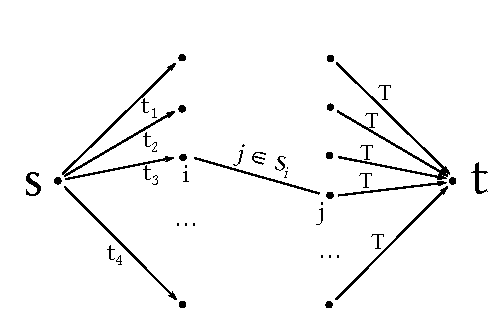
\includegraphics{img/max_flow_jobs.pdf}
   \caption{Job assignment problem}
  \end{center}
 \end{figure}

We create a graph with three layers. We have one $s$ource which is connected to every job. Every job is connected to every worker that can complete this job. All workers are connected to one destination $t$.

\[
  u((s, i)) = t_i  \quad i \in \set{1, 2, \ldots, n}
\] \[
  u((i, j)) = T \fall i, j \text{ with } j \in S_i
\] \[
  u(j, t) = T \fall j \in \set{1, 2, \ldots, n}
\]
where $T$ is a configuration parameter.

Assuming $f_T$ is the maximum flow from $s$ to $t$ in $(G, u, s, t)$. If $\operatorname{value}(f_T) = \sum_{i=1}^n t_i$. We claim: If worker $j$ completes portion $f(i, j)$ of job $j$ $\forall i, j$ then all jobs are completed within time $T$
\[
  [0, T_\text{max}] \sum t_i = T_\text{max}
\]

\dateref{27th of Oct 2014}

Assignment:
\begin{enumerate}
  \item Worker $j$ should complete $f_{i,j}$ units of work of the $i$-th job $\fall i \fall j$.
    \[
      \operatorname{value}{(f)} = \sum_{i=1}^n t_i \quad\Rightarrow\quad f(s, i) = t_i
        \fall \text{job } i
    \] \[
      \underbrace{\Rightarrow}_{\text{flow conservation condition}}
        \sum_{j \in S_i} f_{i,j} = f(s, i) = t_i
    \]
    hence job $i$ will be complete $\fall i$.
  \item Why is everything completed \emph{in time} (ie. $\leq T$)?
    \[
      \fall \text{worker } j:
        \underbrace{\sum_{i,j \in S_i} f(i, j)}_{\text{total working time of worker i}}
        = f(j, t) \leq T
    \]
\end{enumerate}

\subsection{Maximum-flow problem (cont.)}

\paragraph{Linear programming definition of the maximum-flow problem}
%
\given{A network $(G, u, s, t)$. Let $x_e$ be the flow carried by edge $e$ in the network $\fall e \in E(G)$ with $0 \leq x_e \leq u_e$.
\[
  \sum_{e=(i,v)} x_e - \sum_{e=(v,j)} x_e = 0 \fall v \in V(G) \setminus \set{s, t}
\]}
\find{Compute the maximum flow $\sum_{e \in \delta^+(s)} x_e - \sum_{e \in \delta^-(s)} x_e$.}

We are looking for a combinatorial solution.

\textbf{Remark.} MFP is polynomially solvable as linear program eg. via ellipsoid method.

\begin{theorem}
  \label{proposition-4.1}
  MFP always has an optimal solution. Linear programming always provides an optimal solution and is limited by $\sum_{e \in E(G)} u_e$.
\end{theorem}

\textbf{Definition.}
  A \emph{$s$-$t$-cut in $G$} is an edge set $\delta^+(X)$ with $X \subsetneqq V(G), s \in X, t \notin X$. The set of all edges going from $X$ to $X^c$.

The capacity of $\delta^+(x)$ is $u(\delta^+(x)) := \sum_{e \in \delta^+(x)} u_e$.
A minimum $s$-$t$-cut is a $s$-$t$-cut with smallest possible capacity.

\begin{theorem}
  \label{lemma-4.2}
  $\forall A \subsetneqq V(G)$ with $s \in A, t \notin A$ and for every $s$-$t$-flow it holds that:
  \begin{enumerate}
    \item $\operatorname{value}{(f)} = \sum_{e \in \delta^+(A)} f(e) - \sum_{e \in \delta^-(A)} f(e)$
    \item $\operatorname{value}{(f)} \leq \sum_{e \in \delta^+(A)} u_e$
  \end{enumerate}
\end{theorem}

\begin{proof}
  \begin{itemize}
    \item Firstly, \[
        \operatorname{value}(f)
        = \sum_{e \in \delta^+(s)} f_e - \sum_{e \in \delta^-(s)} f_e
        = \sum_{v \in A} \left(
          \underbrace{\sum_{e \in \delta^+(v)} f_e - \sum_{e \in \delta^-(v)} f_e}%
            _{= 0 \fall v \neq s}
        \right)
      \] \[
        = \sum_{e \in \delta^+(A)} f_e - \sum_{e \in \delta^-(A)} f_e
      \]

      All edges in $A$ (that stay in $A$) cancel each other out
      (incoming = $+1$, outgoing = $-1$).
    \item Secondly, \[
      \sum_{e \in \delta^+(A)} f_e - \sum_{e \in \delta^-(A)} f_e
      \leq \sum_{e \in \delta^+(A)} u_e
      = u(\delta^+(A))
    \]
  \end{itemize}
\end{proof}

\textbf{Remark.}
  From theorem~\ref{lemma-4.2} (2) it follows that
  \[
    \underbrace{\max\set{\operatorname{value}(f)}}_{\text{f: \flow st}} \leq
    \underbrace{\min{u(\delta^+(A))}}_{\text{A: $s$-$t$-cut}}
  \]

\index{residual network}
\textbf{Definition.} \emph{(dt. ``Inkrementnetzwerk'', residual network)}
  Assume a network $(G, u, s, t)$ and a \flow st $f$. Define the set of edges as a multiset:
  \[
    \overleftrightarrow E = \set{e: e \in E(G)} \cup \set{\overleftarrow e := (j, i): (i, j) \in E(G)}
  \]
  In words ``all edges and edges in opposing directions including duplicates''.
  We now consider the new graph
  \[
    \overleftrightarrow G = (V(G), \overleftrightarrow E)
  \] \[
    G_f := (V(G), \set{e \in \overleftrightarrow E: u_f(e) > 0})
  \] \[
      \text{ where } u_f(e) \text{ is remaining capacity defined as }
  \] \[
      u_f(e) = \left\{\begin{array}{lc}
        u_e - f_e & e \text{ is edge in forwards direction} \\
        f_{\overleftarrow e} & e \text{ is edge in direction backward } (f_{\overleftarrow e} = f_e) \\
      \end{array}\right.
  \]
  $(G_f, u_f, s, t)$ is then called ``residual network''.

\begin{figure}[ht]
 \begin{center}
  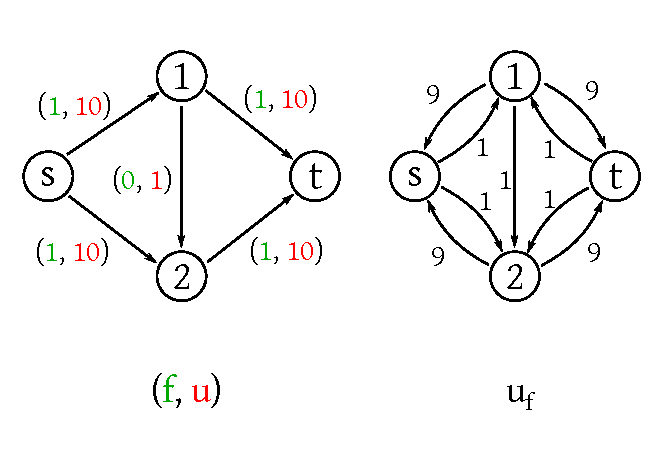
\includegraphics{img/residual_graph.pdf}
  \caption{Residual network}
 \end{center}
\end{figure}

\textbf{Remark.} $2\rightarrow 1$ was not introduced in $G_f$, because $u_f = 0$

A directed \gath st in $G_f$ is called \emph{augmented path}.

\begin{figure}[ht]
 \begin{center}
  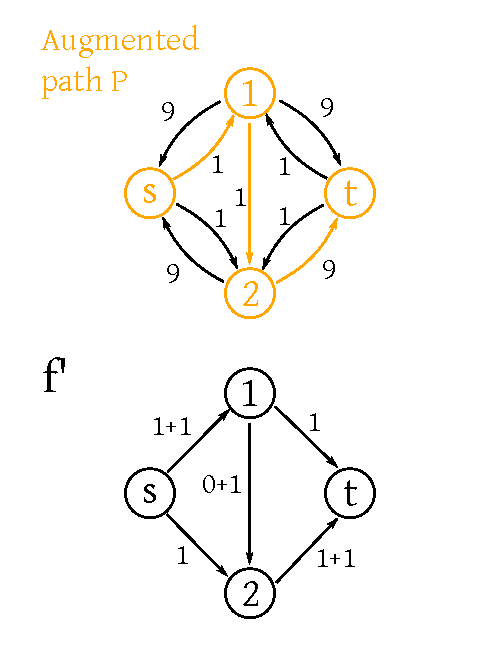
\includegraphics{img/augmented_path.pdf}
  \caption{Augmented path}
 \end{center}
\end{figure}

How do you augment a path?
\[
  f'(e) = \left\{\begin{array}{lc}
    f(e) + \delta  & e \in P \cap E^+ \\
    f(e) - \delta  & e \in P \cap E^- \\
    f(e)           & e \notin P
  \end{array}\right.
\] \[
  f' := f \oplus P \qquad \text{ with } \delta := \min_{e \in E(P)} {u_f(e)}
\]
$f'$ is called augmented path along $P$.

\begin{center}
 \begin{tabular}{cl}
  $P \cap E^+$ & forward edge in path \\
  $P \cap E^-$ & backward edge in path
 \end{tabular}
\end{center}

Show:
\begin{enumerate}
  \item $f'$ is a flow
  \item $\operatorname{value}(f') = \operatorname{value}(f)$
\end{enumerate}

\begin{figure}[ht]
 \begin{center}
  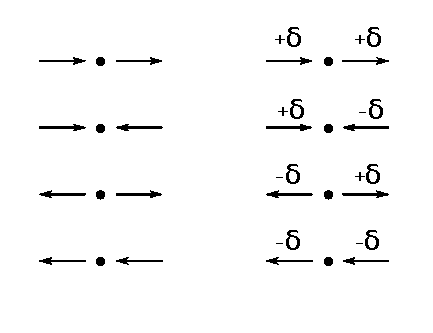
\includegraphics{img/f_is_a_flow.pdf}
  \caption{$f'$ is a flow}
 \end{center}
\end{figure}

Let $e \in P \cap E^+$.
\[
  0 \leq f'(e) \leq u(e)
\] \[
  0 \leq f(e) + \delta \leq u(e)
\] \[
  0 \leq f(e) + \delta \leq f_e + u_e - f(e)
\]

Let $e \in P \cap E'^-$.
\[
  0 = f(e) - f(e) \leq f'(e) = f(e) - \delta \leq u(e)
\] \[
  \operatorname{value}(f')
    = \sum_{e \in \delta^+(s)} f'(e) - \sum_{e \in \delta^-(s)} f'(e)
    = f'(e_0) + \sum_{e \in \delta^+(s)} f'(e) - \sum_{e \in \delta^-(s)} f'(e)
\]

Let $e_e \in \delta^-(s) \cap P = \operatorname{value}(f) + \delta > \operatorname{value}(f)$.

\begin{center}
  Flow augmented by $\delta$ along path $P$ such that the value increases.
\end{center}

\textbf{Remark.}
  If $f$ is a max \flow st, then there is no \gath st in $G_f$.
  If there would be a \gath st $P$ then $f' = f \oplus P$ is better than $f$ (contradiction).

\begin{theorem}\label{lemma-4.3}
  Let $(G, u, s, t)$ be a network and $f$ be a flow. If there is no \gath st in $G_f$,
  then $f$ is optimal. Hence $\operatorname{value}(f)$ is at maximum.
\end{theorem}

\begin{proof}
  Let $A = \set{v \in V(G): v \text{ is reachable from s in } G_f}$.
  $A$ defines a cut between a set $A$ containing $s$ and a set $B$ containing $t$ with $t \notin A$.
  An edge on the border of those sets must satisfy $f(e) = u(e)$ (\emph{saturating edge}),
  otherwise $u(e) - f(e) > 0$ and the edge would be part of $G_f$.

  $A$ defines a $s$-$t$-cut $\delta^+(A)$.
  \[
    u(\delta^+(A)) = \sum_{e \in \delta^+(A)} u_e
  \] \[
    \operatorname{value}(f) = \underbrace{\dots}_{\text{theorem~\ref{lemma-4.2} (a)}}
      = \sum_{e \in \delta^+(A)} f(e) - \sum_{e \in \delta^-(A)} f(e)
  \]
  So this end going from set $B$ to set $A$ has $f(e) = 0$ otherwise
  $\overleftarrow{e}$ is in $G_f$. It follows that $u(\delta^+(A)) = \operatorname{value}(f)$.

  So $f$ is optimal (assumption that cut $\geq$ flow, hence equality, won't get better)
\end{proof}

\begin{theorem} \label{satz-4.4}
  (\emph{Max flow, min cut problem}, Ford \& Fulkerson, 1956)
  Let $(G, u, s, t)$ be a network than there exists a maximum \flow st $f$
  and a minimum cut ($s$-$t$-cut) $\delta^+(A)$ with $\operatorname{value}(f) = u(\delta^+(A))$.
  Especially the value of a maximum flow and the capacity of a minimum $s$-$t$-cut is equal.
\end{theorem}

\subsection{Algorithm by Ford \& Fulkerson}

\begin{proof}
  Directly follows from theorems~\ref{lemma-4.2} and \ref{lemma-4.3}.
\end{proof}

\begin{algorithm}
  \caption{Algorithm by Ford \& Fulkerson}
  \label{fnf-algo}
  \given{$G, u, s, t$}
  \find{max \flow st}
\begin{algorithmic}[1]
  \State Set $f(e) = 0 \fall e \in E(G)$
  \While{$\exists$ \gath st $P$ in $G_f$}
    \State $f = f \oplus P$
  \EndWhile
  \State \Return $f$
\end{algorithmic}
\end{algorithm}

\begin{figure}[!ht]
 \begin{center}
  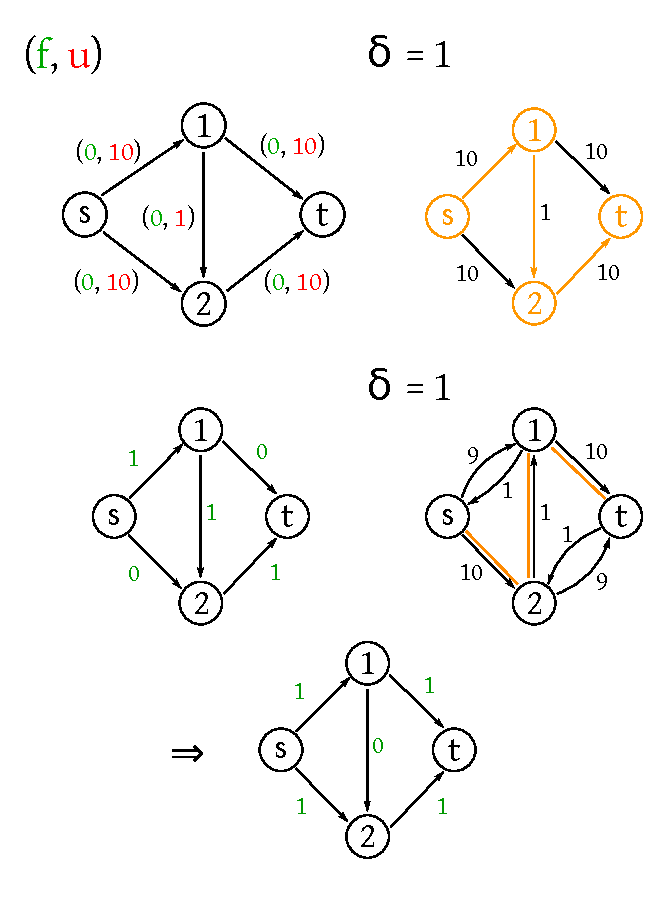
\includegraphics{img/ff_algo.pdf}
  \caption{Ford \& Fulkerson algorithm}
 \end{center}
\end{figure}

As a result many steps are required. Better paths would be $(s, 2, t)$ or $(s, 1, t)$ instead of using $1$--$2$.

\paragraph{Conclusions of F\&F algorithm}
If $u_0 \in \mathbb{Z}_+$ then F\&F algorithm terminates.
After at most $U(\card{V(G)} - 1)$ iterations, where $U = \max_{e \in \delta^+(s)} u_e$, because
\begin{enumerate}
  \item Firstly
    \[
      \operatorname{value}(f)
        \leq \sum_{e \in \delta^+(s)} f(e)
        \leq \sum_{e \in \delta^+(s)} U
        \leq U \cdot (\card{V(G)} - 1)
    \]
  \item Secondly the flow value is increased by $\delta$ in every iteration; where $\delta \geq 1$ because $\delta > 0$ and $\delta \in \mathbb{Z}$.
\end{enumerate}

If $u_e \in Q_+$ then affiliation to $u_e \in \mathbb{Z}_+$ (multiply all capacities with common denominator).

If $u_0 \in Q_+$ then F\&F algorithm must not terminate. It also must not converge and if it does converge, it must not converge towards optimality. So the algorithm might create a series $f_n$ with $\operatorname{value}_{n\rightarrow\infty}(f) \nrightarrow \text{opt}$.

In the algorithm the series converges only if it converges towards optimality.

\dateref{28th of Oct 2014}

\subsubsection{Analysis}
%
\begin{center}
  \begin{tabular}{ll}
    Runtime per iteration:  & $\mathcal{O}(n)$ determination of a \gath st \\
                            & (eg. breadth-first search) if such one exists \\
    Number of iterations:   & $\mathcal{O}(U(n-1)) = \mathcal{O}(Un)$
  \end{tabular}
\end{center}

Total runtime (for $u_e \in \mathbb{Z}_+ \fall e \in E(G):$
\[
  \mathcal{O}(mnU)
\]
\begin{center}
  pseudo-polynomial runtime
\end{center}

\begin{theorem}[Flow decomposition theorem, Galler 1956, Ford and Fulkerson 1962]
  \label{satz-4.5}
  Let $(G, u, s, t)$ be a network and $f$ be a \flow st. Then $\exists$ a family
  $\mathcal{P}$ of \gath sts and a family $\mathcal{C}$ of cycles in $G$ and the
  weights in $\mathcal{P} \cup \mathcal{C} \rightarrow \mathbb{R}_+$
  ($P \mapsto w(P), C \mapsto w(C)$) such that
  \begin{align*}
    f(e) = \sum_{P \in \mathcal{P} \cup \mathcal{C}: e \in E(P)} w(P) \fall e \in E(G)
  \end{align*}
  \begin{align*}
    \operatorname{value}(f) = \sum_{p \in \mathcal{P}} w(P)
      \quad\text{and}\quad
      \card{\mathcal{P}} + \card{\mathcal{C}} \leq \card{E(G)}
  \end{align*}
\end{theorem}

\begin{proof}
  Induction on number of flow-carrying edges, ie. $\card{ e \in E(G): f(e) > 0 }$. \\
  \begin{hypothesis}
    No flow-carrying edge: trivial (select some \gath st and sort by value)
  \end{hypothesis}
  \textbf{Induction step.}

  Let $i=0$ and $(V_0, w_0) \in E(G)$ otherwise $f(v_0, w_0) > 0$.
  If $w_0 \neq t \exists (w_0, w_1) \in E(G)$ with $f(w_0, w_1) > 0$.
  If $w_1 \notin \set{t, v_0, w_0}$ then $i = i + 1$ and repeat this step until $t$ is reached or some vertex is repeated (cycle case).

  Analogously you can think of $(v_1, v_0) \in E(G)$ with $f(v_1, v_0) > 0$. If $v_1 \notin \set{s, v_0, w_0, w_1, \ldots, w_k}$ then repeat the step until $s$ is reached or some cycle gets created.

  \begin{figure}[ht]
   \begin{center}
    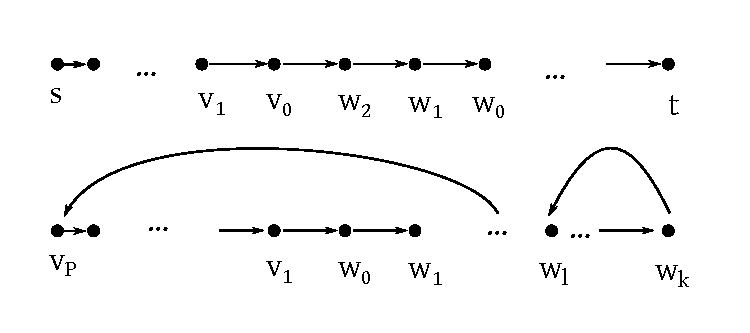
\includegraphics{img/flow_decomposition_theorem.pdf}
    \caption{Flow decomposition theorem}
   \end{center}
  \end{figure}

  This construction provides either a flow-carrying \gath st $P$ or a flow-carrying cycle $C$. Case distinction:
  \begin{enumerate}
    \item $w(P_2) = \min_{l \in E(P_0)} f(e)$ and \[
          f(e) = \begin{array}{lc}
            f(e) - w(P)  & e \in E(P), \forall e \in E(G) \\
            f(e)         & e \notin E(P) \forall e \in E(G)
          \end{array}\]
    \item $w(C_2) = \min_{e \in E(C)} f(e)$ analogously.
  \end{enumerate}

  $f'$ is a \flow st with at least one flow-carrying edge less.
  With the induction hypothesis $f'$ can be decomposed, hence $\exists \mathcal{P}_1(\mathcal{C}_1)$ family of \gath sts (cycles) and $w: \mathcal{P}_1 \cup \mathcal{C}_1 \rightarrow \mathcal{R}_+$ with $f'(e) = \sum_{P \in \mathcal{P}_1 \cup \mathcal{C}_1, e \in E(P)} w(P)$ and $\operatorname{value}(f') = \sum_{p \in \mathcal{P}_1} w(P)$ and $\card{\mathcal{P}_1 \cup \mathcal{C}_1} \leq E(G)$.

  \begin{enumerate}
    \item
      \[
        \mathcal{P} := \mathcal{P}_1 \cup \set{P_0}, \mathcal{C} := \mathcal{C_1}
      \] \[
        \underbrace{f(e) = f'(e) + w(P_0)}_{\text{if } e \in E(P)}
          = \sum_{P \in \mathcal{P}_1 \cup \mathcal{C}_1, e \in E(P)} w(P) + w(P_0)
          = \sum_{P \in \mathcal{P} \cup \mathcal{C}, e \in E(P)} w(P)
      \]
    \item
      \[
        \mathcal{P} := \mathcal{P}_1, \mathcal{C}
          := \mathcal{C_1} \cup \set{C_0} \text{ with corresponding weights}
      \] \[
        \operatorname{value}(f) = \operatorname{value}(f') + w(P_0)
          = \sum_{P \in \mathcal{P}_1} w(P) + w(P_0)
          = \sum_{P \in \mathcal{P}} w(P)
      \]
    \item
      $\card{\mathcal{P} \cup \mathcal{C}} \leq \card{E(G)}$ because the induction step will be executed at most $\card{E(G)}$ times. In every step a new non-flow-carrying edge is created and in every step $i$ $(\mathcal{P}_i \cup \mathcal{C}_i)$ is incremented by one and we can start with $\mathcal{P} \cup \mathcal{C} = \diameter$ for flow $f \equiv 0$.
  \end{enumerate}
\end{proof}

\subsection[Edmonds and Karp algorithm]{Edmonds and Karp algorithm (E\&K)}
\label{ch-4.3}
%
This algorithm distinguishes from F\&F only by the selection of the \gath st: In every iteration $i$ a shortest \gath st $P_i$ in $G_{f_i}$ is selected (shortest in terms of number of edges).

\begin{algorithm}
  \caption{Edmonds and Karp algorithm}
  \label{ek-algo}
  \given{$G, u, s, t$}
  \find{max \flow st}
\begin{algorithmic}[1]
  \State Let $f(e) = 0 \fall e \in E(G)$
  \State Determine a shortest $f$-augmenting path $P$
    \label{ek-step-redo}
  \If{$P$ does not exist}
    \State \Return $f$
  \EndIf
  \State
    Determine $\gamma = \min_{e \in E(P)} u_f(e)$.
    Augment $f$ along $P$ by $\gamma$
  \State \Goto{ek-step-redo}
\end{algorithmic}
\end{algorithm}

\begin{figure}[!ht]
 \begin{center}
  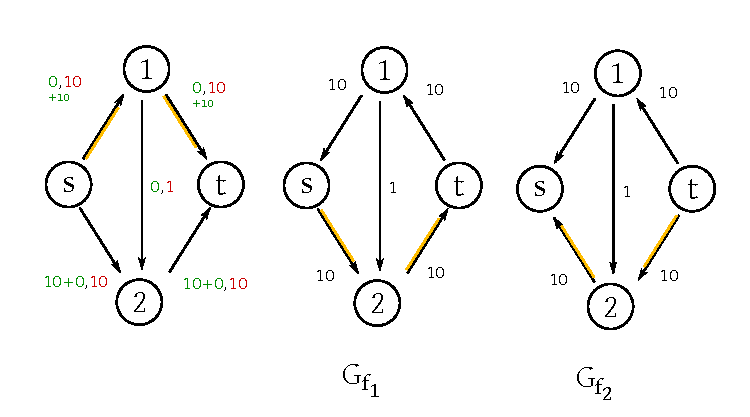
\includegraphics{img/ek_algorithm1.pdf}
  \caption{Drawing for EK algorithm}
 \end{center}
 \begin{center}
  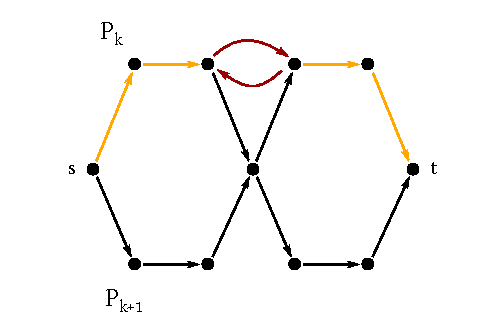
\includegraphics{img/ek_algorithm.pdf}
  \caption{Drawing for EK algorithm}
 \end{center}
\end{figure}

\begin{theorem}\label{lemma-4.6}
  Let $f_0, f_1, \ldots, f_k, \ldots$ be a sequence of flows created by the E\&K algorithm, where $f_{i+1} = f_i + P_i$ and $P_i$ is a shortest \gath st in $G_{f_i} \fall i$. Then it holds that
  \begin{itemize}
    \item $\card{E(P_k)} \leq \card{E(P_{k+1})} \fall i$
    \item $\card{E(P_k) + z \leq \card{E(P_r)}}$ for all $k < r$ such that $P_k \cup P_r$ contains at least one pair of edges of opposing direction.
  \end{itemize}
\end{theorem}

\begin{proof}
  \begin{enumerate}
    \item
      Let $G_k := (V, E_k)$ where $E_k = P_k \cup P_{k+1} \setminus \set{\text{pairs of edges in opposing direction}}$.
      It holds that $E_k \subseteq E(G_{f_k})$ (where $G_{f_k}$ is an incremental network to $f_k$), because $P_k \cup P_{k+1} \subseteq E(G_{f_k}): P_k \subseteq E(G_{f_k})$ is obvious.

      \textbf{Assumption.}
        $\exists e \in P_{k+1} \setminus E(G_{f_k}): e \in E(G_{f_{k+1}})$. Hence $e$ was added to the incremental network in the $k$-th iteration.
    \item
      So $e$ is an edge of opposing direction of an edge of $P_k$. This is a contradiction because $e \notin E_k$. So $E_k \subseteq E(G_{f_k})$ holds.

      Add two artificial edges $(t, s)$ to $E_k$ ($G_k = (V, E_k)$) and retrieve $\bar G_k$. $\bar G_k$ is eulerian (in a directed sense), ie. $\degree^-_{\hat C_k}(v) = \degree^-_{\hat C_k}(v) \fall v$.
      $\Rightarrow \hat G_k$ can be decomposed into edge-disjoint cycles. Let $C_1(C_2)$ be the cycles that contain the artificial edges $1$ and $2$.

      Let $P_1$ and $P_2$ be the edge-disjoint \gath sts in those cycles $C_1$ and $C_2$.

      $P_1$ and $P_2$ are in $\hat G_k$ and do not require any artificial edges.

      \[
        P_1\ \text{and}\ P_2 \in E(G_k) \subseteq E(G_{f_k})
      \]

      \[
        2 \card{E(P_k)} \leq \card{E(P_1)} + \card{E(P_2)}
      \] \[
          \leq \card{E(G_k)} \leq \card{E(P_k)} + \card{E(P_{k+1})}
      \] \[
          \Rightarrow \card{E(P_k)} \leq \card{E(P_{k+1})}
      \]

    \item
      It suffices to show this statement for $k < r$, where $P_r$ and $P_i$ contain no edges of opposing direction $\fall k < i < r$.

      \textbf{Reasoning.} Let $P_{k+1}$ be the last path $P_k, P_{k+1}, \ldots, P_{k+i}, \ldots, P_r$ with edges of opposing direction to $P_r$.
      From $\card{E(P_{k+1})} + 2 \subseteq \card{E(P_r)}$ it follows (with $\card{E(P_k)} \leq \card{E(P_{k+1})}$):
      \[
        \card{E(P_k)} + 2 \leq \card{E(P_{k+1}) + 2 \leq  \card{E(P_r)}}
      \]
      We assume without loss of generality that $P_k$ and $P_r$ contain edges of opposing direction but not $P_i, P_r \fall k < i < r$.
      Construct $G_k$ with all edges from $P_k \cup P_r$ without pairs of edges of opposing direction. It holds that $E(G_k) \subseteq E(G_{f_k})$ because otherwise $\exists e \in P_r: \card{E(G_{f_k})}$ hence $e$ is not contained in $E(G_{f_k})$, but in $E(G_{f_r})$. Hence $e$ was added in iterations $k$, $k+1$, \dots, $r-1$. So $e$ has an edge of opposing direction in $P_k$, $P_{k+1}$, \dots, $P_{r-1}$.
  \end{enumerate}
\end{proof}

\begin{figure}[ht]
 \begin{center}
  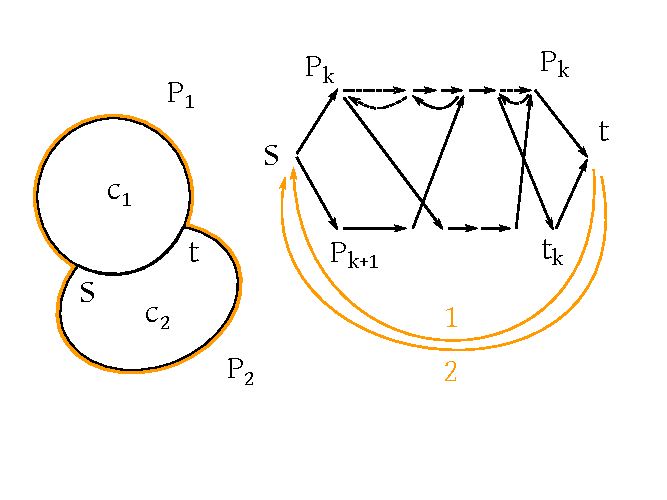
\includegraphics{img/ek_algorithm2.pdf}
  \caption{Edmonds and Karp algorithm}
 \end{center}
\end{figure}

Analogously as in case $a$ we find 2 edge-disjoint \gath sts $P_1$ and $P_2$ in $G_{f_k}$:
\[
  2 \card{E(P_k)} \leq \card{E(P_1)} + \card{E(P_2)} \leq \card{E(G_k)} \leq \card{E(P_k)} + \card{E(P_r)} - 2
\] \[
  \Rightarrow \card{E(P_k)} + 2 \leq \card{E(P_r)}
\]

\begin{theorem}\label{satz-4.6}
  (Edmonds and Karp, 1972)
  The algorithm of Edmonds and Karp requires at most $\frac{nm}2$ augmented paths (equals to the number of iterations) and determines a maximum flow correctly. The algorithm has a runtime complexity of $\mathcal{O}(m^2 \cdot n)$.
\end{theorem}

\begin{proof}
  \index{Bottleneck edge}
  An edge $e \in P$ (where $P$ is an augmented path in $G_f$) is called \emph{bottleneck edge} if
  \[
    \min_{g \in E(P)} u_f(g) = u_f(e)
  \]
  \textbf{Question.}
    How often can some edge $e$ occur as bottleneck edge during the algorithm run?

    Let $e$ be a bottleneck edge in $P_k$. Then it holds that $e \notin E(G_{f_{k+1}})$. If the edge becomes a bottleneck edge again of $P_k$ with $e > k$, then the edge goes into the residual network; hence the edge is of opposing direction of another edge of the previous augmented path; without loss of generality to an edge of $P_k$:
    \[
      \card{E(P_k)} + 2 \leq \card{E(P_e)}
    \]
    Introduction of $e$ as bottleneck $\Rightarrow$ augmented path gets extended.
    \begin{center}
      at most $n - 1$ extensions \\
      $\Rightarrow$ per $e$ at most $n-1$ bottleneck edges \\
      $\Rightarrow$ number of iterations: $\mathcal{O}(m\cdot n)$
    \end{center}
\end{proof}

\dateref{3rd of November 2014}

\subsubsection{Runtime analysis}

The number of iterations is $\mathcal{O}(nm)$ because every edge $\mathcal{O}(n)$ becomes a bottleneck at one point in time. A more precise upper bound is $\frac{n}{4}$.

Let $k$ be the iteration in which $e = (v, w)$ becomes a bottleneck edge. Then let $r > k$ be the index of the next iteration in which $e$ becomes a bottleneck edge again.

\begin{figure}[ht]
 \begin{center}
  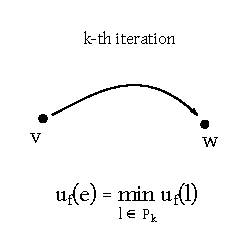
\includegraphics{img/ek_bottleneck.pdf}
  \caption{Edmonds and Karp algorithm -- Bottlenecks}
 \end{center}
\end{figure}

\[
  k+1 \text{ iteration with } e \notin G_{f_{k+1}}
\] \[
  \Rightarrow \quad \overleftarrow{e} \in G_{f_p}(k+1 \leq p)
\]
\begin{center}
  \dots must be satisfied and flow must go through $\overleftarrow{e}$ such that $e$ can recur in $G_f$.
\end{center}

\[ E(P_p) \geq E(P_k) + 2 \]
\[ r \text{ iterations} \Rightarrow E(P_r) \geq E(P_p) + 2 \]
\[ e \in G_{f_r}: E(P_r) \geq E(P_k) + 4 \]

Every time when $e$ becomes a bottleneck edge, the length of the shortest \gath st by at least $4$. So $e$ is at most $\frac n4$ times a bottleneck edge.
\[
  \#\text{iterations} \leq 2m \frac n4 = \frac{mn}2
\] \[
  (|E| \cup |\overleftarrow{E}| \leq 2m)
\]

This bound is the best we can achieve. In some cases this bound is reached.

\textbf{Total runtime:}
  $\mathcal{O}(m)$ per iteration $\times \mathcal{O}(mn)$ iterations = $\mathcal{O}(m^2n)$

\subsection{Blocking flows and Dinitz's algorithm (1970)}
%
\given{Network $(G, u, s, t)$ and $s$-$t$-flow $f$. Its level graph $G_f^L$ is a subgraph of $G_f$ with
\[
  V(G_f^L) := V(G_f), E(G_f^L) := \set{e = (x, y) \in E(G_f):
    \operatorname{dist}_{G_f}(s, x) + 1 = \operatorname{dist}_{G_f}(s, y)
  }
\]}

\textbf{Observation.}
  $G_f^L$ is ayclic. $v_0 \rightarrow v_1 \rightarrow v_2 \rightarrow v_k \rightarrow v_0$. $\operatorname{dist}(v_0) = \operatorname{dist}(v_0) + k$ is a contradiction.

Constructable with $\mathcal{O}(m)$ runtime (eg. BFS).

\textbf{Definition.} $s$-$t$-flow $f$ is called \emph{blocking}, if graph $(V(G), \set{e \in E(G_F^L): f(e) < u(e)})$ does not contain a \gath st.

\clearpage
Not every blocking flow is optimal.

\begin{itemize}
  \item First example:
    \begin{figure}[!ht]
      \begin{center}
       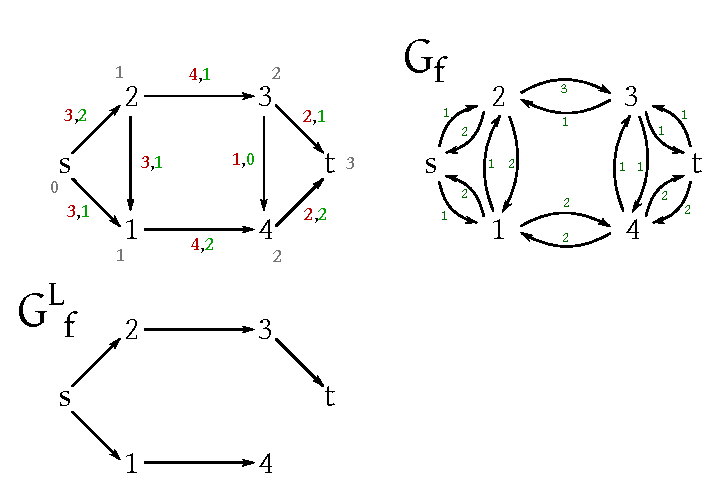
\includegraphics{img/blocking_flows_a.pdf}
       \caption{Example (a) graphs}
      \end{center}
    \end{figure}

    \[
      \exists \text{\gath st in }  G^L_f
        \Rightarrow f \text{ is non-blocking}
    \]

  \item Second example:
    \begin{figure}[!ht]
      \begin{center}
       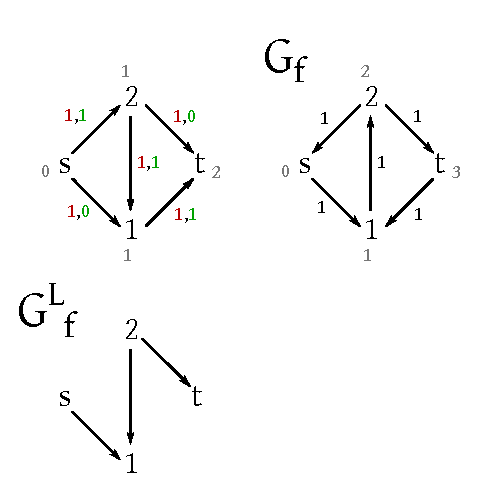
\includegraphics{img/blocking_flows_b.pdf}
       \caption{Example (b) graphs}
      \end{center}
    \end{figure}

    \[
      \nexists \text{\gath st}
        \Rightarrow f \text{ blocking, but there is a \gath st in } G_f \Rightarrow \text{non-optimal}
    \]

    \[
      \text{ in } (V(G), \set{e \in E(G^L_f): f(e) < u(e)})
    \]
    \begin{figure}[!ht]
      \begin{center}
       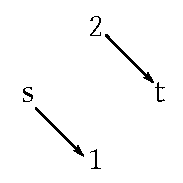
\includegraphics{img/blocking_flows_b_in.pdf}
       \caption{Example (b) schematic}
      \end{center}
    \end{figure}
\end{itemize}


\begin{algorithm}
  \caption{Dinitz's algorithm}
  \label{dinitz-algo}
  \given{Network $(G, u, s, t)$}
  \find{$s$-$t$-flow $f$ with maximum value}
\begin{algorithmic}[1]
  \State Let $f(e) := 0 \fall e \in E(G)$
  \State Build level-graph $G^L_f$ (subgraph of $G_f$)
  \State Determine a blocking flow $f'$ in $G^L_f$. If $f' = 0$, then stop ``$f$ is optimal''.
  \State Augment $f \oplus f'$, goto step 2
  \[
    f \oplus f'(e) = \begin{cases}
      f(e) + f'(e) & e \in E(G) \\
      f(e) + f'(e) & e \in \overleftarrow{E}(G)
    \end{cases}
    \fall e \in E(G)
  \]
\end{algorithmic}
\end{algorithm}

Recall that
  \[ \card{E(P_{k+1})} \geq \card{E(P_k)} \]
  \[ E(G_k) \subseteq E(G_{f_k}) \]

\begin{theorem}\label{satz-4.7}
  Dinitz' algorithm finds a maximum flow in $\mathcal{O}(n^2m)$ runtime.
\end{theorem}

\begin{proof}
  \textbf{Runtime analysis.}
  Number of iterations: $\mathcal{O}(n-1)$

  Because length of shortest \gath st increases after every iteration by at least 1.
  This is analogous to proof of theorem~\ref{satz-4.4}: The blocking flow ``contains'' all
  shortest paths of same length.

  Determination of a blocking flow in $G^L_f$ in $\mathcal{O}(nm)$ runtime (see practicals)

  \[
    \mathcal{O}(n^2 m)
  \]

  \textbf{Correctness.}
  Blocking flow $=0$ in $G^L_f \Rightarrow$ no \gath st in $G_f \Rightarrow f$ is optimal.

  (Sleator \& Tarjan, 1984).
    $\mathcal{O}(m \log{n})$ for determination of a blocking flow in a level graph.
\end{proof}

\subsection{Goldberg \& Tarjan: Push-Relabel algorithm}
%
Algorithm by Goldberg \& Tarjan (1988).

\index{preflow}
\index{active vertex (Push-relabel algorithm)}
\textbf{Definition.}
  Let $(G, u, s, t)$ be a network with source $s$ and sink $t$.
  $f: E(G) \rightarrow \mathbb{R}_+$ is called \emph{preflow} if $f(e) \leq u(e) \fall e \in E(G)$
  and $\operatorname{ex}_f(v) \geq 0 \fall v \in V(G) \setminus \set{s}$.
  A vertex $v \in V(G) \setminus \set{s, t}$ is called \emph{active} if $\operatorname{ex}_f(v) > 0$.

\textbf{Idea.}
  Work with preflow $f$ satisfying $\exists$ \gath st in $G_f$ and try iteratively to reduce the excess for active vertices until no more active vertices exist.

\textbf{Definition.}
  Let $(G, u, s, t)$ be a network. A mapping $\psi: V(G) \rightarrow \mathbb{Z}_+$ is called \emph{distance marker} if $\psi(t) = 0$ and $\psi(s) = n$ and $\psi(v) \leq \psi(w) + 1 \fall (v, w) \in G_f$.

An edge $e = (v, w) \in E \cup \overleftarrow{W}$ is called \emph{permitted edge} if $\psi(v) = \psi(w) + 1$.

\textbf{Observation.}
  If $\psi$ is a distance marker then $\psi(v)$ is a lower bound for the number of edges in a shortest \gath vt in $G_f$.

  \[ v_0 \rightarrow v_1 \rightarrow \dots \rightarrow v_k=t \]
  \[
    \psi(v_0) \leq \psi(v_1) + 1
      \leq \psi(v_2) + 1 + 1
      \leq \ldots
      \leq \underbrace{\psi(v_k)}_{\psi(t) = 0} + k = k
  \]

Algorithm applies push or relabel operations. Starts with preflow which saturates all edges $(s, v)$ ($f(s,v) = u(s,v)$) $\Rightarrow$ in $G_f$ there is no outgoing edge from $s$ $\Rightarrow \nexists$ \gath st
\[
  f(e) = 0 \text{ if } e \cap \set{s} = \diameter
\] \[
  f(v,s) = 0
\]

Has active vertex? If not, then done (optimality criterion satisfied)

\begin{algorithm}
  \caption{Push-Relabel algorithm (book: page~201)}
  \label{push-relabel-algo}
  \given{$G, u, s, t$}
  \find{Maximum \flow st $f$}
\begin{algorithmic}[1]
  \State $f(e) := u(e) \fall e \in \delta^+(s)$
  \State $f(e) := 0 \fall e \in E(G) \setminus \delta^+(s)$
  \State $\psi(s) := n := \card{V(G)}$ and $\psi(v) := 0 \fall v \in V(G) \setminus \set{s}$
  \While{there exists an active vertex}
    \State Let $v$ be an active vertex
    \If{no $e \in \delta_{G_f}^+(v)$ is a permitted edge}
      \State Relabel
    \Else
      \State Let $e \in \delta_{G_f}^+(v)$ be some permitted edge
      \State $\operatorname{Push}(e)$
    \EndIf
  \EndWhile
\end{algorithmic}
\textbf{Push(e)}
\begin{algorithmic}[1]
  \State Let $\gamma = \min\set{\operatorname{ex}_f(v), u_f(e)}$ where $e$ starts in $v$
  \State Augment $f$ along $e$ in $\gamma$
\end{algorithmic}
\textbf{Relabel(v)}
\begin{algorithmic}[1]
  \State Let $\psi(v) := \min\set{\psi(w) + 1: (v, w) \in \delta^+_{G_f}(v)}$
\end{algorithmic}
\end{algorithm}

Condition for $\psi(v) \leq \psi(w) + 1$ is only satisfied for edges in $G_f$.
\[
  \begin{array}{ll}
    \text{permitted:} & \psi(v) = \psi(w) + 1 \\
    \text{not permitted:} & \psi(v) < \psi(w) + 1
  \end{array}
\]

\begin{theorem}\label{proposition-4.8}
  The push-relabel algorithm has two invariants:
  \begin{itemize}
    \item $f$ is always an $s$-$t$-preflow
    \item $\psi$ is always a corresponding distance marker
  \end{itemize}
\end{theorem}

\begin{proof}
  After initialization both invariants are given (trivial case).

  \begin{description}
    \item[PUSH of edge $(v, w)$]
      \[ f'(e) = f(e) + y \]
      \[ \operatorname{ex}_{f'}(v) = \operatorname{ex}_f(v) - y \geq 0 \]
      \[ \operatorname{ex}_{f'}(w) = \operatorname{ex}_f(w) + y \geq 0 \]

      Distance marker: If $(v, w)$ is cancelled, condition is still satisfied.

      If $(w, v)$ is added, then $\psi(w) \leq \psi(v) + 1$ but PUSH only if permitted:
      $\psi(v) = \psi(w) + 1$.

    \item[RELABEL] does not influence $f$, stays a preflow
      \[ \psi(v) = \min\set{\psi(w) + 1: w \in \delta^+(v)} \]
      \[ \Rightarrow \psi(v) \text{ increases} \]

      $G_f$ does not change. Inequations can only be invalidated for edges.

      \[
        \begin{array}{lll}
          v \rightarrow w & \psi(v) \leq \psi(w) + 1 & \text{$\psi(v)$ is never increased too much} \\
          w \rightarrow v & \psi(w) \leq \psi(v) + 1 & \text{$\psi(v)$ is larger (which is fine)} \\
        \end{array}
      \]
  \end{description}
\end{proof}

\dateref{4th of November 2014}

\begin{theorem}\label{lemma-4.9}
  Let $f$ be a preflow and $\psi$ be a distance marker in regards of $f$. Then the following statements hold:
  \begin{enumerate}
    \item $s$ is reachable from every active vertex $v$ in $G_f$.
    \item If $v, w \in V(G)$ with $w$ being reachable from $v$ in $G_f$,
          then $\psi(v) \leq \psi(w) + n - 1$
    \item $t$ is not reachable in $G_f$
  \end{enumerate}
\end{theorem}

\begin{proof}
  \begin{itemize}
    \item Part 1 of proof:
      Let $v$ be active. Let $R$ be the set of vertices reachable vertices in $G_f$ from $v$.
      The following does not exist:
      \begin{center}
        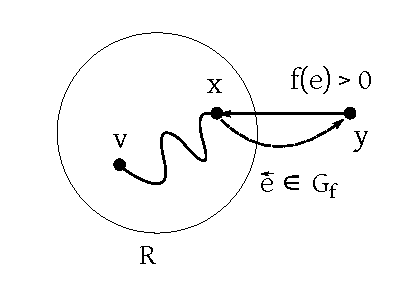
\includegraphics{img/lemma-4_9-proof-a.pdf}
      \end{center}

      \textbf{Observation.} $\fall e = (y, x) \in \delta^-(R)$ it holds that $f(e) = 0$. Otherwise $y \in R$ which contradicts.
      \[ \operatorname{ex}_f(w) = \sum_{e \in \delta^-(w)} f(e) - \sum_{\delta^+} f(e) \]
      \[ \sum_{w \in R} \operatorname{ex}_f = \sum_{e \in \delta^-(R)} f(e) - \sum_{e \in \delta^+(R)} f(e) \leq 0 \]
      \[ f(e) = 0 \text{ in case } e \in \delta^-(R) \]
      \[ \text{For $v$ it holds that } \operatorname{ex}_f(v) > 0 \text{ because $v$ is active} \]
      \[ \Rightarrow \exists w \in R \text{ with } \operatorname{ex}_f(w) < 0 \]
      \[ \Rightarrow w = s \Rightarrow s \in R \]
    \item Part 2 of proof:
      \begin{center}
        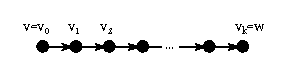
\includegraphics{img/lemma-4_9-proof-b.pdf}
        \textit{\gath vw in $G_f$}
      \end{center}
      \[
        \psi(v_0) \leq \psi(v_1) + 1
          \leq \psi(v_2) + 1 + 1 \dots
          \leq \underbrace{\psi(w)}_{v_k = w} + k
          \leq \psi(w) + n - 1
      \]
      $k:$ length $\leq n-1$ because of $n$ vertices in $G$.
    \item Part 3 of proof - contradiction: Assume that $t$ is reachable from $s$
      \[
        \Rightarrow \exists \text{\gath st in } G_f
        \stackrel{b}{\Rightarrow} \underbrace{\psi(s)}_{n} \leq \underbrace{\psi(t)}_{0} + n - 1
        \Rightarrow n \leq n - 1
        \Rightarrow \text{contradiction}
      \]
  \end{itemize}
\end{proof}

\begin{theorem}\label{satz-4.10}
  When PR algorithm terminates, $f$ is a maximum \flow st.
\end{theorem}

\begin{proof}
  No active vertices at termination $\Rightarrow$ preflow is flow and from Theorem~\ref{lemma-4.9}~(c) ``t is not reachable from s in $G_f$'' is an invariant of the algorithm. Hence at termination the optimality criterion is satisfied.
\end{proof}

\begin{theorem}\label{lemma-4.11}
  (number of relabel operations)
  \begin{itemize}
    \item $\fall v \in V(G): \psi(v)$ is increased in every relabel operation by at least one (strong monotonicity, no decrement)
    \item $\psi(v) \leq 2n - 1$ is an invariant $\forall v \in V(G)$
    \item No vertex exists which is relabelled more than $2n - 1$ times. Hence the maximum number of relabel operations is $2n^2 - n$
  \end{itemize}
\end{theorem}

\begin{proof}
  \begin{itemize}
    \item Active $v$ has edges to $w_1, w_2, \ldots, w_k$.
      \[ \psi(v) < \psi(w_i) + 1 \qquad \Rightarrow \text{edge not permitted} \]
      Relabel:
      \[ \overline{\psi(v)} = \min_{i: w_i \in \delta^+(v)} \psi(w_i) + 1 = \psi(w_l) + 1 > \psi(v) \]
    \item Initialization: $\psi(v) = 0 \fall v \neq s$, $\psi(s) = n$. Initialization okay.

      Inequation can possibly be invalidated by relabelling?
      \[
        \operatorname{Relabel}(v)
          \Rightarrow v \text{ active}
          \stackrel{\text{theorem~\ref{lemma-4.9} (1)}}{\Rightarrow} s \text{ is reachable in $G_f$ from } v
      \] \[
        \stackrel{\text{theorem~\ref{lemma-4.9} (2)}}{\Rightarrow}
          \psi(v) \leq \psi(s) + n - 1
          = n + n - 1 = 2n - 1
      \]
    \item Follows trivially from the previous 2 points
  \end{itemize}
\end{proof}

\textbf{Definition.}
  Let $e = (x, y)$. $\push(e)$ is called \emph{saturating} push operation if
  \[ y = \min\set{\operatorname{ex}_f(x), u_f(e)} = \underbrace{u_f(e)}_{\neq \operatorname{ex}_f(x)} \]
  otherwise $\push(e)$ is a non-saturating operation.

\begin{theorem}\label{lemma-4.12}
  The number of saturating push operations is $2nm$.
\end{theorem}

\begin{proof}
  Consider $e = (v, w)$. How many times will a saturating push operation $\push(e)$ be executed?

  \begin{center}
    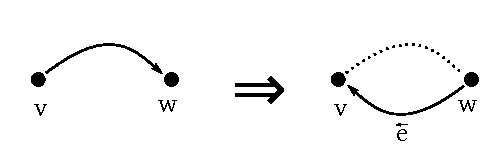
\includegraphics{img/saturating_push.pdf}
  \end{center}

  Edge must be be reintroduced in $G_f$ to be pushed again.
  \[ \psi(v) = \psi(w) + 1 \]

  Before the next $\push(e)$, $e$ must be added to $G_f$.
  How? This is only possible through $\push(\overleftarrow{e})$. It holds:
  \[
    \psi'(w) = \psi'(v) + 1  \quad\Rightarrow\quad  \psi'(w) \geq \psi(v) + 1
  \]

  So $\phi(w)$ has been incremented by at least 2.
  If the next $\push(e)$ happens, it furthermore holds that
  \[
    \psi''(v) = \psi''(w) + 1 \geq \psi(w) + 2 + 1
  \]
  In conclusion: Between every two continuous saturating push operations $\push(e)$, $\phi(v)$ was incremented by at least 2.
  From theorem~\ref{lemma-4.11} (b) we conclude that we have at most $n-1$ jumps (by 2) of $\phi(v)$. This also means that we have at most $n$ saturating push operations.

  So for all edges of $E \cup \overleftarrow{E}$ we have at most $2mn$ saturating push operations.
\end{proof}

\begin{theorem}\label{lemma-4.13}
  \emph{Number of non-saturating push operations.}
  The number of non-saturating push operations is $\mathcal{O}(n^2m)$.
\end{theorem}

\begin{proof}
  Let $A$ be the set of all active vertices.
  \[
    D := \sum_{v \in A} \psi(v) \qquad \text{potential function}
  \]
  Start with $D = 0$. At termination $A = \diameter, D = 0$.
  How does $D$ change with execution of various operations?

  \begin{itemize}
    \item Non-saturating operation $\push(v, w)$:

      Transitions:
      \[
        \begin{array}{rclcc}
          \text{active}     & \rightarrow & \text{active} & \quad & \text{D is less or equal} \\
          \text{non-active} & \rightarrow & \text{active} & \quad & \triangle D = -\psi(v) + \psi(w) = -(\psi(w) + 1) + \psi(w) = -1 \\
                            &             &               &       & \text{D is less} \\
        \end{array}
      \]

    \item Saturating operation $\push(v, w)$:
      Transitions:
      \[
        \begin{array}{rrclcc}
          w: & \text{active}     & \rightarrow & \text{active} & \quad & \text{D stays the same} \\
          w: & \text{non-active} & \rightarrow & \text{active} & \quad & \text{D stays the same or increases} \\
          v: & \text{active}     & \rightarrow & \text{active} & \quad & \text{D stays the same or increases}
        \end{array}
      \]
  \end{itemize}

  Relabel $D$ increases, because $\psi(v)$ increases.

  So in conclusion only non-saturating push is responsible for decreasing $D$.

\end{proof}

By how much does $D$ increment during the algorithm's run?
\[
  2nm \text{ saturating pushes } + 2n^2 - n \text{ relabels}
\]
It increases with $\mathcal{O}((nm + n^2) \cdot n) = \mathcal{O}(n^2m)$.

\begin{theorem}\label{lemma-4.14}
  \emph{Better analysis for number of non-saturating push operations. Cheriyan and Mehlhorn 1999.}
  If the algorithm always select an active vertex with maximum $\psi(v)$, then the push-and-relabel algorithm only requires $8n^2 \sqrt{m}$ non-saturating push operations.
\end{theorem}

\begin{theorem}\label{satz-4.15}
  The push-and-relabel algorithm solves the maximum-flow problem correctly and can be implemented with $\mathcal{O}(n^2 \sqrt{m})$ runtime.
  (with selection of active vertices as in Theorem~\ref{lemma-4.14})
\end{theorem}

\begin{proof}
  Correctness is given in theorem~\ref{satz-4.10} and theorem~\ref{proposition-4.8}. What about the runtime?

  We use a doubly-linked list $L_i$ where
  \[
    L_i := \set{v \in V(G); v \text{ is active}; \psi(v) = i \quad 0 \leq i \leq 2n - 1}
  \]

  At the begining we start with $L_0 := $ all active vertices.
  Let $i = 0$ (at the beginning) and scan $L_i$ for some selected $v \in L_i$.
  As an invariant $i$ is the greatest index $j$ with $L_j \neq 0$.

  \begin{itemize}
    \item $i$ must be updated in constant time
    \item lists as well
  \end{itemize}

  \[ k = \psi(v) \]
  Relabel: \[ \psi(v) = \min_{w\in\delta^+(v)}{\set{\psi(w) + 1}} = \hat k \]
  \[ \mathcal{O}(\card{\delta^+(v)}) \]

  If $k > i$, then $i = k$.
  \[ L_{\hat k} = L_k \cup \set{v} \]
  \[ L_k = L_k \setminus \set{v} \]

  $\push(e): v \rightarrow w$
  \begin{itemize}
    \item $v$ = active, switch to
      \begin{itemize}
        \item active
        \item inactive: $L_{\psi(v)} = L_{\psi(v)} \setminus \set{v}$
      \end{itemize}
    \item $w$ = active, switch to
      \begin{itemize}
        \item active: $i = \psi(v) \land L_{\psi(v)} = \diameter, i \leftarrow i', i' \text{ next } L_{i'} \neq \diameter$
      \end{itemize}
    \item $w$: inactive, switch to
      \begin{itemize}
        \item active: $L_{\hat \psi(w)} = \hat L_{\psi(w)} \cup \set{w}, \hat\psi(w) > i$ then $i = \hat\psi(w)$
      \end{itemize}
  \end{itemize}

  Data structure $A_v \fall v \in V(G)$ is doubly linked.
  \[ A_v = \set{w \in \delta^+(v): (v, w)\ \text{permitted}} \]

  Saturating push: edge is removed from $A_v$:
  \[ A_v := A_v \setminus \set{w} \]
  Unsaturating push: $A_v$ stays unmodified
  \[ A_v := A_v \setminus \set{w} \]

  \[
    \operatorname{Relabel}(v) := \psi(w) = \min_{w\in\delta^+(v)}{\set{\psi(w) + 1}}
      = \psi(w_e) + 1
      \Rightarrow A_v = A_v \cup \set{w_e}
  \]

  Per edge $2n-1$ times.
  \[ 2n-1 \mathcal{O}(\bigcup_{v \in V(G)} \card{\delta^+(v)}) \]
  \[ = \mathcal{O}(nm) \]
\end{proof}

\dateref{10th of November 2014}

\subsection{Minimum-capacity cut problem}
\label{section-4.5}
%
\given{Instance $(G, u, s, t)$, $u: t \rightarrow R_t$}
\find{A $s$-$t$-cut in $G$ with minimum capacity}

\textbf{Simple solution.}
  Determine maximum flow $f$ from $s$ to $t$ and all reachable vertices $v$ from $s$ in $G_f$.
  Let $C$ be that vertex. From the maximum-flow min-cut theorem it follows that
  \[
    \operatorname{value}(f) = u(\delta(L)) \quad\rightarrow\quad \delta(c) \text{ minimum $s$-$t$-cut}
  \]
  If you want to compute one minimum cut per pair $(s, t)$, solve ${1 \choose 2}$ max-flow problems
  and determine the corresponding cuts (as above)
  \[
    {n \choose 2} \mathcal{O}(n^2 \sqrt{n})
  \]
  $(n-1)$ flow computations actually suffice; see Gomor-Hu tree (1962).

\textbf{For undirected graphs.}
  Let $G$ be an undirected graph and $u: E(G) \rightarrow \mathbb{R}_+ \fall s, t \in V(G)$.
  Let $\lambda_{s,t}$ be the \emph{local node connectivity} defined as minimum capacity of a splitting $s$-$t$-cut. The \emph{node connectivity of a graph} is defined as $\min_{s, t \in V(G), s \neq t} \lambda_{s,t}$ where $\lambda_{s,t}$ is computed with $u(e) = 1 \fall e \in E(G)$.

\begin{figure}[ht]
 \begin{center}
  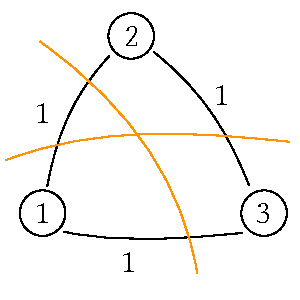
\includegraphics{img/vertex_connection.pdf}
  \caption{Vertex connection}
 \end{center}
\end{figure}
\[
  \lambda_{1,2} = \lambda_{2,3} = \lambda_{1,3} = 2
\] \[
  \min{\set{\lambda_{12}, \lambda_{23}, \lambda_{13}}} = 2
\] \[
  \Rightarrow \text{ node connectivity of } G = 2
\]

\textbf{Alternative definition:}
  $G = (V, E)$ is called $t$-node-connected if the graph $G$ stays connected after removal of $t-1$ vertices. The node connectivity number $K(G)$ of a graph $G$ is defined as $K(G) = \max_{t \in \set{1, 2, \ldots, \card{V(G)} - 2}} \set{t: G \quad t \text{ node connectivity}}$.

\begin{theorem}\label{lemma-4.5}
  For every triple of vertices $i, j, k \in V(G)$ (G is an undirected graph) it holds that
  \[
    \lambda_{i,k} \geq \min{\set{\lambda_{i,j}, \lambda_{j,k}}}
  \]
\end{theorem}

\begin{proof}
  Let $\delta(C)$ be a minimum $i$-$k$-cut with $\lambda_{i,k} = u(\delta(C))$.
  If $j \in C$ then $\lambda_{j,k} \leq u(\delta(C)) = \lambda_{i,k}$.
  If $j \in V(G) \setminus C$ then $\lambda_{i,j} \leq u(\delta(C)) = \lambda_{i,k}$.
  So $\lambda_{i,k} \geq \lambda_{j,k}$ or $\lambda_{i,k} \geq \lambda_{i,j}$.
  $\Rightarrow \lambda_{i,k} \geq \min{\set{\lambda_{j,k}, \lambda_{j,i}}}$.
\end{proof}

\textbf{Remark.}
  The condition of theorem~\ref{lemma-4.5} is required for $(\lambda_{i,j})_{i,j \in 1, 2, \ldots, n}$ node connectivity numbers of a graph with vertex set $\set{1, 2, \ldots, n}$.
  But this condition is not sufficient; hence $\exists$ numbers $\lambda_{i,j}$ for $i,j \in \set{1, 2, \ldots, n}$ that satisfy these conditions, but cannot be retrieved as node connectivity number of a graph.

  If $\lambda_{i,j} = \lambda_{j,i} \forall i,j \in \set{1, 2, \ldots, n}$ and the conditions of theorem~\ref{lemma-4.5} hold, then it holds that a graph $G$ with $V(G) = \set{1, 2, \ldots, n}$ and $\exists u: E(G) \rightarrow \mathbb{R}_+$, such that $\lambda_{i,j}$ for $i,j \in \set{1, 2, \ldots, n}$ that are local node connectivity numbers of $(G, u)$.

\textbf{Definition.}
  Let $G$ be an undirected graph and $u: E(G) \rightarrow \mathbb{R}_+$, $E$ in tree $T$ is called Gomory-Hu-tree of $(G, u)$ iff
  \[
    V(T) = V(G) \land \lambda_{s,t} = \min_{e \in E(P_{s,t})} u(\lambda_G (c_e)) \fall s,t \in V(G), s \neq t
  \]

\begin{figure}[ht]
 \begin{center}
  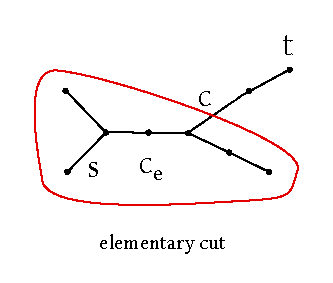
\includegraphics{img/fundamental_cut.pdf}
  \caption{Elementary cut}
 \end{center}
\end{figure}

\[
  K_{3,3} \qquad n \equiv 1
\] \[
  \lambda_{s_i,t_j} = \lambda_{s_1, t_1} = 3 \forall i \in \set{1, 2, 3}, j \in \set{1, 2, 3}
\] \[
  \lambda_{s_1,s_2} = \lambda_{s_1,s_3} = \lambda_{s_2,s_3} = \lambda_{t_1,t_2}
    = \lambda_{t_2,t_3} = \lambda_{t_1,t_3} = 3
\] \[
  \lambda_{s_2, t_2} = \min\set{
    \underbrace{u(\delta(c_{e_1}))}_{=3},
    \underbrace{u(\delta(c(e_2)))}_{=3}
  } = 3
\]

\begin{figure}[ht]
 \begin{center}
  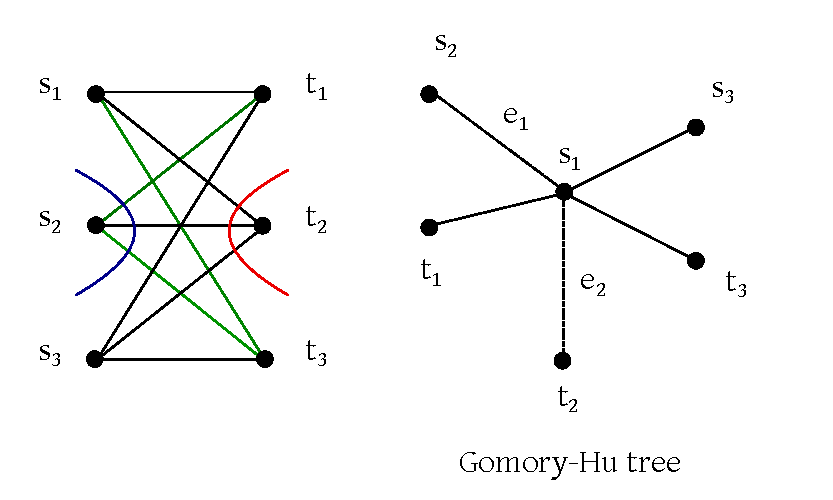
\includegraphics{img/gomory_hu.pdf}
  \caption{Gomory Hu algorithm}
 \end{center}
\end{figure}

\subsection{Gomory-Hu algorithm}
\textbf{Basic idea:}
  Select vertex pair $s, t \in V(G)$ and determine its minimum $s$-$t$-cut $\delta(A)$ where $B := V(G) \setminus A$. Contract $A$ (or $B$) to one vertex. Then select $s'$, $t' \in B$ (or $A$).

  Build a minimum $s'$-$t'$-cut $\delta(A')$ in contracting graph $G'$ with $V(G') \setminus A'$. Observe that a minimum cut in the contracting graph corresponds to a minimum cut in the original graph. Repeat this step as long as not-separated vertices exist.

\begin{figure}[ht]
 \begin{center}
  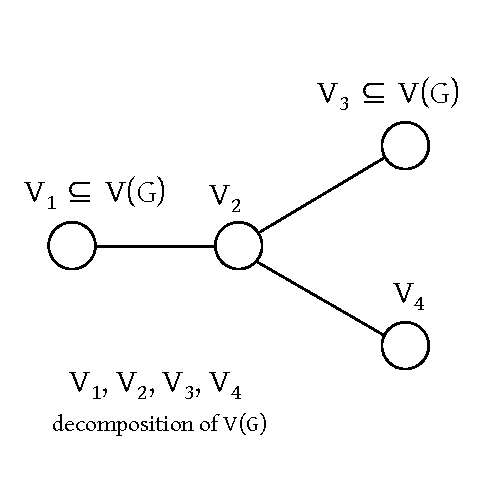
\includegraphics{img/gomory_hu_algo_idea.pdf}
  \caption{Gomory Hu algorithm idea}
 \end{center}
\end{figure}

% TODO: verify
% I think the following applies:
%  w are the weights in the Gomory Hu tree
%  u are the edge weights in the original graph
\begin{algorithm}
  \caption{Gomory Hu algorithm}
  \label{gomory-hu-algo}
  \given{undirected graph $G$, $u: E(G) \rightarrow \mathbb{R}_+$}
  \find{A Gomory-Hu tree $T$ for $(G, u)$}
\begin{algorithmic}[1]
  \State $V(T) = \set{V(G)}$, $E(T) = \diameter$ (a vertex that corresponds to all vertices in $G$)
  \State Choose $X \in V(T)$ with $\card{X} \geq 2$. If $\nexists X$, then goto step 6.
  \State Choose $s,t \in X$ ($s \neq t$), $H$ as connected component $C$ of $T-X$ \\
         Select $S_c := \bigcup_{Y \in V(C)} Y$. $(G', u')$ results from $(G, u)$ by contraction of $s_c$ to a single vertex $V_c$ for every connected component $C$ of $T-x$. So $V(G') = X \cup \set{V_c: c \text{ connected component of } T-X}$.
  \State
    Determine the minimum $s$-$t$-cut $\delta(A')$ in $(G', u')$. Let $B' = V(G') \setminus A'$.
    Set
    \begin{align*}
      A &= \bigcup_{V_c \in A' \setminus X} S_c \cup (A' \cap X) \\
      \intertext{and}
      B &= \bigcup_{V_c \in B' \setminus X} S_c \cup (B' \cap X)
    \end{align*}
  \State
    Set $V(T) := (V(T) \setminus X) \cup (A \cap X) \cup (B \cap X)$.
  \State
    For every edge $e = \set{X, Y} \in E(T)$ incident with $X$ do, \\
    \hspace{20pt} if $V \subseteq A$, set $e' := \set{A \cap X, Y}$ \\
    \hspace{20pt} else $e' := \set{B \cap X, Y}$. \\
    \hspace{20pt} Set $E(T) := (E(T) \setminus e) \cup \set{e'}$, $w(e') := w(e)$. \\
    \hspace{20pt} Set $E(T) := E(T) \cup \set{A \cap X, B \cap X}$ with \\
    \hspace{40pt} $w(\set{A \cap X, B \cap W}) = u'(\delta_G, (A'))$. \\
    \hspace{20pt} Goto step 2.
  \State Replace all $\set{X} \in V(T)$ by $X$ and all $\set{\set{X}, \set{Y}}$ by $\set{X, Y}$.
\end{algorithmic}
\end{algorithm}

\begin{theorem}\label{lemma-4.16}
  Let $G$ be an undirected graph and $u: E(G) \rightarrow \mathbb{R}_+$.
  Let $s, t \in V(G)$ and $\delta(A)$ be a minimum $s$-$t$-cut in $(G', u')$.
  $(G', u')$ results from $(G, u)$ by contraction of $A$ by a single vertex $K$.
  Let $s', t' \in V(G) \setminus A$. Then it holds that
  \[
    \forall \min{\text{s'-t'-cuts}}: \delta(K \cup \set{A}) \text{ is }
      \delta(K \cup A) \text{ a minimum s'-t'-cut in } (G, u)
  \]
\end{theorem}

\textbf{Remark.}
  It's a minimal cut. It does not preserve capacity.

\begin{figure}[ht]
 \begin{center}
  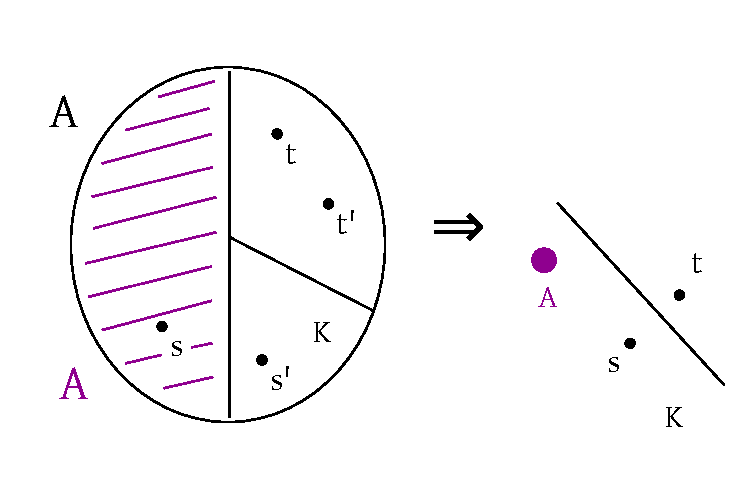
\includegraphics{img/lemma_4_16.pdf}
  \caption{Lemma 4.16}
 \end{center}
\end{figure}

So $K$ is the set of non-contracting vertices that are on the same halfplane like the $s'$-$t'$-cut like $A$.

\begin{proof}
  We show: there exists a minimum $s'$-$t'$-cut $\delta(A')$ in $(G, u')$ with $A \subseteq A'$.
  Let $\delta(c)$ be a minimum $s'$-$t'$-cut in $(G, u)$. Without loss of generality let $s \in C$.
  If $A \subseteq C$, we are done. Otherwise build a second minimum $s'$-$t'$-path in $G$, which contains $A$.
  It holds that
  \[
    u(\delta(A)) + u(\delta(c)) \geq u(\delta(A \cap C)) + u(\delta(A \cup C))
  \]
  Because $\delta(A \cap C)$ is a $s$-$t$-cut $G$ it holds that
  \[
    u(\delta(A \cap c)) \geq \lambda_{s,t} = u(\delta(A))
  \] \[
    u(\delta(A \cap C) \leq u(\delta(c)) = \lambda_{s',t'} \Rightarrow u(\delta(A \cap C)) = \lambda_{s',t'}
  \] \[
    A \cap C \text{ is minimum s'-t' cut with } A \cap C \subseteq A
  \]
\end{proof}

\begin{figure}[ht]
 \begin{center}
  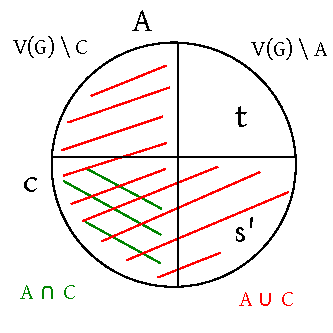
\includegraphics{img/lemma_4_16_proof.pdf}
  \caption{Lemma 4.16 proof}
 \end{center}
\end{figure}

\textbf{Definition.}
  $f: 2^M \rightarrow \mathbb{R}$ where $M$ is the set and $2^M$ is the power set of $M$.
  $f$ is called submodular if $f(A \cap B) + f(A \cup B) \leq f(A) + f(B) \fall A, B \in 2^M$.

\begin{theorem}\label{lemma-4.17}
  After every iteration of step 4, the following conditions hold:
  \begin{itemize}
    \item $A \mathop{\dot{\cup}} B = V(G)$
    \item $E(A, B)$ is a minimum $s$-$t$-cut in $(G, u)$
  \end{itemize}
  \[
    A, B \subseteq V(G)  \qquad  E(A, B) := \set{e \in E(G): e = (x, y) \quad x \in A, y \in B}
  \]
\end{theorem}

\noproof{lemma-4.17}

\begin{theorem}\label{lemma-4.18}
  Invariant of the algorithm:
  \[
    w(e) = u(\delta_G(\bigcup_{z \in C_e} Z)) \fall e \in E(T)
  \]
  where $c_e$ and $V(T) \setminus c_e$ are the two connected components of $T - e$.
  Furthermore it holds that
  \[
    \forall e = \set{P, Q} \in E(T)
      \quad \exists p \in P
      \quad \exists q \in Q \text{ with } \lambda_{p,q} = w(e)
  \]
\end{theorem}

\noproof{lemma-4.18}

\begin{theorem}\label{satz-4.19}
  The Gomory-Hu algorithm works correctly.
  Every undirected graph contains a Gomory-Hu tree which can be computed in runtime $\mathcal{O}(n^3 \sqrt{m})$.
\end{theorem}

\noproof{satz-4.19}

\subsection{Minimum capacity of a cut in an undirected graph / MA-order}

\given{$G$ as undirected graph, $u: E(G) \rightarrow \mathbb{R}_+$}
\find{
  Determine a $A^* \subsetneqq V(G), A^* \neq \diameter$ such that
  \[
    u(\delta(A^*)) = \min_{A \subsetneqq V(G), A \neq \diameter} u(\delta(A))
  \]
}

\textbf{Solution 1.}
  Let $s \in V(G)$ be random. Determine $\lambda_{s,t} \forall t \in V(G) \setminus \set{s}$.
  The cut minimizing $\lambda_{s,t}$ is the optimal cut.
  The solution with Gomory-Hu algorithm: The optimal cut is computed using the edge $e^* \in \text{ GH-tree T with } w(e^*) = \min_{e \in E(T)} w(e)$.

\textbf{Solution 2.}
  \index{MA-order}
  (Frank 1994, Stoer \& Wagner 1997.)
  Let $G$ be an undirected graph with $u: E(G) \rightarrow \mathbb{R}_+$.
  An order $v_1, v_2, \ldots, v_u$ of vertices is called \emph{MA-order} (maximum adjacency order)
  if $\fall i \in \set{1, 2, \ldots, n}$ it holds that:
  \[
    \sum_{e \in E(\set{v_1}, \set{v_1, v_2, \ldots, v_{i-1}})} u(e)
      = \max_{j \in \set{i, i+1, \ldots, n}} \sum_{e \in E(\set{v_1}, \set{v_1, \ldots, v_{i-1}})} u(e)
  \]
  This order is not distinct.

\begin{theorem}\label{proposition-4.20}
  In an undirected graph $G$ with $u: E(G) \rightarrow \mathbb{R}_+$ we can compute a MA-order in $\mathcal{O}(m + n\log{n})$ time.
\end{theorem}

\begin{proof}
  Algorithmically. Let $\alpha(v) := 0 \fall v \in V(G)$. Apply the following solution for $i = 1$ to $n$.
  Select some $v_i \in \argmax{\set{\alpha(v): v \in V(G) | \set{v_1, \ldots, v_{i-1}}}}$.
  ``tie branching arbitrarily''.
  \[
    \alpha(v) := \alpha(v) + \sum_{e \in E(\set{v_i}, \set{v})} u(e)
      \qquad\forall v \in V(G) \setminus \set{v_1, v_2, \ldots, v_i}
  \]
\end{proof}

Proving correctness is trivial this is an invariant:
\[
  \alpha(v) = \sum_{c \in E(\set{v}, \set{v_1, \ldots, v_i})}
    \qquad \forall v \in V(G) \setminus \set{v_1, \ldots, v_i}
\]

Time complexity:
Fibonacci heaps with key $-\alpha(v)$.

\begin{center}
  \begin{tabular}{lcc}
    delete min   & $\mathcal{O}(\log{n})$ & (amortized) \\
    insert       & $\mathcal{O}(1)$       & \\
    decrease-key & $\mathcal{O}(1)$       & (armortized)
  \end{tabular}
  \[ \Rightarrow \mathcal{O}(m + n \log{n}) \]
\end{center}

\begin{theorem}\label{lemma-4.21}
  Let $G$ be an undirected graph with $u: E(G) \rightarrow \mathbb{R}_+$ and MA-order $u_1, \ldots, u_n$.
  Then it holds that
  \[
    \lambda_{v_{n-1}, v_n} = \sum_{e \in E(\set{v_n}, \set{v_1, \ldots, v_{n-1}})}
  \]
\end{theorem}

\begin{proof}
  Proving direction ``$\leq$'' is trivial. For ``$\geq$'' via induction over $\card{V(G)} + \card{E(G)}$.
  \begin{description}
    \item[induction base] $\card{V(G)} \leq 2$ is trivial.
    \item[induction step]
      $\card{V(G)} \geq 3$. Without loss of generality $(V_{n-1}, V_{n}) \notin E(G)$,
      because if $e \in E(G)$ with $e = (v_{n-1}, v_n)$. Then $e$ is optimal cut between $v_{n-1}$
      and $v_n$. Furthermore $e \in E(\set{v_n}, \set{v_1, \ldots, v_{n-1}})$.
      Hence removal of edge $e$ reduces both sides of theorem~\ref{lemma-4.21} by $u(e)$.
      Followingly the induction hypothesis is applicable.

      Let
      \[
        R := \sum_{e \in E(\set{v_n}, \set{v_1, \ldots, v_{n-2}})} u(e)
          \stackrel{(u_n, u_{n-1}) \notin E}{=}
          \sum_{e \in E(\set{v_n}, \set{v_1, \ldots, v_{n-1}})} u(e)
      \]

      \[
        (v_1, \ldots, v_n) \text{ is MA-order } \in G
          \Rightarrow (v_1, \ldots, v_{n-1}) \text{ is MA-order } \in G \setminus {v_n}
      \]

      From the induction hypothesis for $G - \set{v_n}$ it follows that
      \[
        \lambda_{n-2,n-1} =
          \sum_{e \in E(\set{v_{n-1}}, \set{v_1, \ldots, v_{n-2}})} u(e)
        \geq
          \sum_{e \in E(\set{v_{n}}, \set{v_1, \ldots, v_{n-2}})} u(e)
        = R
      \] \begin{align}
        \Rightarrow \lambda^G_{v_{n-2}, v_{n-1}} \geq R
      \end{align}

      \[
        v_1, v_2, \ldots, v_{n-2}, v_n \text{ is a MA-order in } G-\set{v_{n-1}}
      \]
      From induction hypothesis it follows:
      \begin{align}
        \lambda^G_{v_{n-2},v_n} \geq \lambda^{G - \set{v_{n-1}}}_{v_{n-2}, v_n}
          = \sum_{e \in E(\set{v_1}, \set{v_1, \ldots, v_{n-1}})} u(e) = R
      \end{align}

      From the last two statements regarding $R$ we conclude,
      \[
        \lambda_{v_{n-1},v_n} := \lambda^G_{v_{n-1}, v_n}
          \geq \min{\set{\lambda^G_{v_{n-1}, v_{n-2}}, \lambda^G_{v_{n-2}, v_{n}}}}
          \geq R
      \]
      (triangle inequation)
  \end{description}
\end{proof}

\begin{theorem}\label{satz-4.22}
  A cut of minimum capacity in an undirected graph $G$
  with $u: E(G) \rightarrow \mathbb{R}_+$ can be computed
  in $\mathcal{O}(nm + n^2 \log{m})$ runtime.
\end{theorem}

\begin{proof}
  Constructive proof.
  Several edges of capacity $u$ with same source and destination can be combined to a single edge.
  So we can can assume wlog no multi-edges.

  Denote $\lambda_G$ as the minimum capacity of a cut in $G$. Let $G_0 := G$. Apply $n$ steps.
  In the $i$-th step ($i = 1, 2, \ldots, n$) select vertex $x, y \in V(G_{i-1})$ with
  \[
    \lambda^{G_{i-1}}_{x,y} = \sum_{e \in \delta_{G_{i-1}}(x)} u(e)
  \]
  It's existence is given by theorem~\ref{lemma-4.21} and $x$ last vertex and $y$ pre-last vertex in concern of a MA-order in $G_{i-1}$.

  Let $y_i = \lambda^{G_{i-1}}_{x,y}$ and $z_i = x \fall i = 1, 2, \ldots, n$.
  Build $G_i$ from $G_{i-1}$ by contraction of edge $(x, y)$.

  \textbf{Observation.}
    \[
      \lambda(G) = \lambda(G_0) = \min{\set{\lambda(G_1), \gamma_1}}
        = \min{\set{\min{\set{\lambda(G_2, \gamma_2)}, \gamma_1}}}
    \] \[
        = \min{\set{\lambda(G_2), \gamma_2, \gamma_1}}
        = \min{\set{\lambda(\underbrace{G_{n-1}}_{=+\infty}), \gamma_1, \gamma_2, \ldots, \gamma_{n-1}}}
    \] \[
        = \min_{i=1,\ldots,n-1} \gamma_i \qquad \text{value of optimal cut}
    \]

    Let $\lambda(G) = \gamma_k = \lambda_{Z_k, \gamma}^{k-1}$ ($z_k$ is a vertex connected by an edge with $y$ and this edge is part of the cut; $z_k$ is alone, but could be a multi-vertex).

    The optimal cut is determine by the subset of the vertex set, that can be contracted in $z_k$.

  \textbf{Complexity.}
    $n$ iterations. Per iteration we compute the MA-order in $\mathcal{O}(m + n \log{n})$ and contraction and defining new capacities takes $\mathcal{O}(n+m)$. This gives us
    \[ \Rightarrow \mathcal{O}(mn + n^2 \log{n}) \]

  \textbf{Example.}

  \begin{figure}[ht]
    \begin{center}
      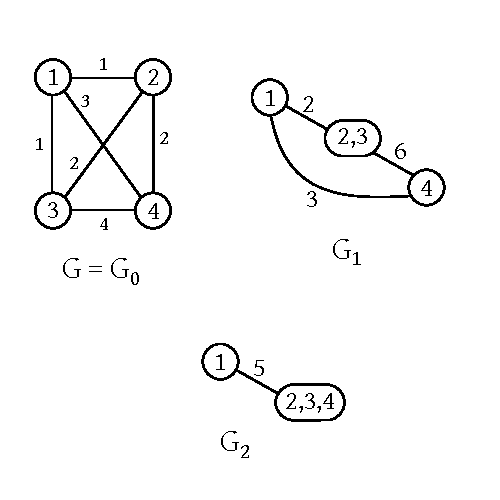
\includegraphics{img/min_capacity_cut.pdf}
      \caption{Example for minimum capacity cut}
    \end{center}
  \end{figure}

  \[
    \text{MA in $G_0$}:
      \underbrace{1}_{\text{arbitrary}},
      \underbrace{4}_{\text{most edges to 1}},
      \underbrace{3}_{y},
      \underbrace{2}_{x}
  \] \[
    z_1 = 2 \qquad y_1 = 1 + 2 + 2 = 5
  \]

  \[
    \text{MA in $G_1$}:
      1,
      \underbrace{4}_{y},
      \underbrace{(2,3)}_{x}
  \] \[
    z_2 = (2, 3) \qquad y_2 = 2 + 6 = 8
  \]

  \[
    \text{MA in $G_2$}:
      \underbrace{1}_y,
      \underbrace{(4,2,3)}_{x}
  \] \[
    z_3 = (4, 2, 3) \qquad y_3 = 5
  \]

  \[
    \gamma(G) = \min\set{\gamma_1, \gamma_2, \gamma_3} = \gamma_1 (\text{or } \gamma_3)
  \]

  In $G_3$ we would have only 1 vertex remaining.
\end{proof}

\section{Flows with minimum costs}
%
\index{b-flow}
\begin{definition}[$b$-flow, offering / demanding vertex]
  Let $G$ be a digraph.
  \[ u: E(G) \rightarrow \mathbb{R}_+ \qquad c: E(G) \rightarrow \mathbb{R} \]
  Let $b: V(G) \rightarrow \mathbb{R}$ with $\sum_{v \in V(G)} b(v) = 0$.
  A \emph{$b$-flow of $G$} is a mapping $f: E(G) \rightarrow \mathbb{R}_+$ such that
  \[ f(e) \leq u(e) \qquad \forall e \in E(G) \quad \text{``capacity restrictions''} \]
  and
  \[
    \sum_{e \in \delta^+(v)} f(e) - \sum_{e \in \delta^-(v)} f(e)
      = b(v) \qquad \forall v \in V(G)
      \qquad \text{flow preservation conditions}
  \]
  hold.

  A $v$ with $b(v) > 0$ is called \enquote{offering vertex}.
  A $v$ with $b(v) < 0$ is called \enquote{demanding vertex}.
\end{definition}


\subsection{Minimum cost flow problem (MCFP/MKFP)}
%
\given{Digraph $G$
\[ u: E(G) \rightarrow \mathbb{R}_+
  \qquad c: E(G) \rightarrow \mathbb{R}
  \qquad b: V(G) \rightarrow \mathbb{R}
\] with $\sum_{v \in V(G)} b(v) = 0$}
\find{Determine a $b$-flow with minimum costs, \\
  ie. the $b$-flow which minimizes $\sum_{e \in E(G)} c(e) f(e)$
}

\textbf{Remark.}
  A $b$-flow is determined by the maximum-flow-problem.

\[
  u(s, v) = \max{\set{0, b(V)}} \fall v \in V(G)
\] \[
  u(v, t) = \max{\set{0, -b(v)}} \fall v \in V(G)
\]

A maximum \flow st $f$ in $G'$ has value $\sum_{v \in V(G)} b(v)$
iff a $b$-flow exists in $G$. If $b$-flow exists, then $f$ restricted by $E(G)$ by $b$-flow.

\begin{figure}[ht]
 \begin{center}
  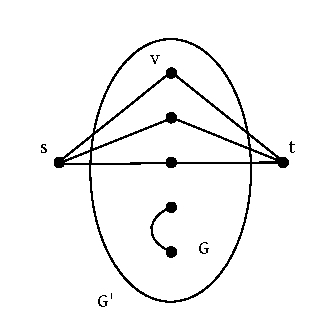
\includegraphics{img/b_flow.pdf}
  \caption{$b$-flow}
 \end{center}
\end{figure}

\textbf{Observation.}
  There exists a max \flow st with value
  \[ \sum_{v \in V(G), b(v) > 0} b(v) \text{ in G'} \]

\begin{figure}[ht]
 \begin{center}
  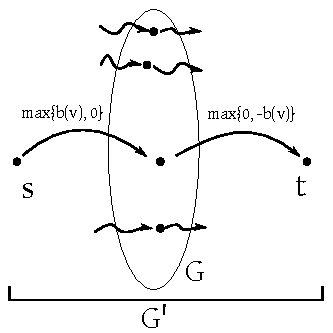
\includegraphics{img/mcfp_observation.pdf}
  \caption{MFCP observation}
 \end{center}
\end{figure}

\[ \Leftrightarrow b-\text{flow in } G \]

$\Rightarrow$ Let $f'$ be a max-$s$-$t$-flow with
\[ \operatorname{value}(f') = \sum_{v \in V(G), b(v) > 0} b(v) \]

Let $f = f'|_{E(G)}$ hence $f: E(G) \rightarrow \mathbb{R}$ with $f(e) = f'(e) \fall e \in E(G)$.
Show that $f$ is a $b$-flow.

\[
  \fall v \in V(G): \sum_{l \in \delta^+_G(v)} f(e) - \sum_{l \in \delta^-_G(v)} f(e)
    = \fall_{e \in \delta^+_G(v)} f'(e) - f'(v, t) - \sum_{e \in \delta^-_G(v)} f'(e)
      + f'(s, v)
\] \[
  = f'(s, v) - f'(v, t) = \max\set{b(v), 0} - \max\set{0, -b(v)}
  = b(v) \Rightarrow f \text{ is $b$-flow}
\]

$\Leftarrow$ Let $f$ be a $b$-flow in $G$.
Construct $f': E(G') \rightarrow \mathbb{R}$ with
\[
  f'(e) = \begin{cases}
    f(e)               & e \in z(G) \\
    \max\set{0, b(v)}  & e = (s, v) \\
    \max\set{0, -b(v)} & e = (v, t)
  \end{cases}
\]

Exercise: Show that $f'$ is an \flow st with value
\[ \sum_{v \in V(G)} \max\set{0, b(v)} = \sum_{v \in V(G), b(v) > 0} b(v) \]

\subsection{The transportation problem}
%
\given{Digraph $G$ with $V(G) = A \dotcup B$ and $E(G) \subseteq A \times B$.
  $b(v) \geq 0 \fall v \in A, b(v) < 0 \fall v \in B, \sum_{v \in V(G)} b(v) = 0$.
  Capacities $u(e) = \infty \fall e \in E(G)$ and $c: E(G) \rightarrow \mathbb{R}$.
}
\find{$b$-flow in $G$ with minimum costs}

\textbf{Remark.}
  Without loss of generality $c(e) \geq 0 \fall e \in E(G)$.
  Otherwise $\alpha$ is large enough ($c(e) + \alpha \geq 0 \fall e \in E(G)$).

\[ c'(e) = c(e) + \alpha \geq 0 \fall e \in E(G) \]

Let $f$ be a $b$-flow in $G$. Compare $c'(f)$ and $c(f)$.
\[
  c'(f)
    = \sum_{e \in E(G)} c'(e) f(e)
    = \sum_{e \in E(G)} (c(e) + \alpha) f(e)
    = c(f) + \alpha \sum_{e \in E(G)} f(e)
\]

Consider
\[
  \sum_{(u,v) \in E(G)} f(u,v)
    = \sum_{u \in V(G)} \sum_{e \in \delta^+_G(u)} f(e)
    = \sum_{u \in A} \left( \sum_{e \in \delta^+_G(u)} f(e) - \sum_{e \in \delta^-_G(u)} f(e) \right)
    = \sum_{u \in A} b(u) =: \overline{b}
\] \[
  c'(f) = c(f) + a\overline{b}
\]

\begin{figure}[ht]
 \begin{center}
  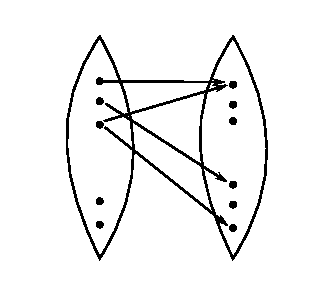
\includegraphics{img/transportation_problem.pdf}
  \caption{Transportation problem}
 \end{center}
\end{figure}

\subsection{An optimality criterion}
%
Let $f$ be a $b$-flow. $G_f$ is defined analogously like in the max-flow problem. Costs in $G_f$:
\[
  c_f: E(G_f) \rightarrow \mathbb{R}
\] \[
  c_f(e) = \begin{cases}
    c(e) & e \in E(G) \\
    -c(e) & \overleftarrow{e} \in E(G)
  \end{cases}
\]

\textbf{Definition.}
  Let $G$ be a digraph with capacity $u: E(G) \rightarrow \mathbb{R}_+$ and let $f$ be a $b$-flow in $G$.
  A \emph{$f$-augmenting cycle} is a cycle in $G_f$.

\begin{theorem}\label{proposition-5.1}
  Let $G$ be a digraph with capacity $u: E(G) \rightarrow \mathbb{R}_+$. Let $f$ and $f'$ be $b$-flows in $G$. Then $g: \overleftrightarrow{E}(G) \rightarrow \mathbb{R}$ with $g(e) = \max\set{0,f'(e) - f(e)}$ and $g(\overleftarrow{e}) = \max\set{0, f(e) - f'(e)} \fall e \in E(G)$ is a \emph{circulation} in $\overleftrightarrow{G} := (V(G), \overleftrightarrow{E}(G))$. Furthermore it holds that $g(e) = 0 \fall e \in \overleftrightarrow E(G) \setminus E(G_f)$ and $c(g) = c(f') - c(f)$.
\end{theorem}

\begin{proof}
  \[ \fall v \in V(\overleftrightarrow{G}) = V(G) \]
  \begin{equation*}
    \sum_{e \in \delta^+_{\overleftrightarrow{G}}(v)} g(e) - \sum_{e \in \delta^-_{\overleftrightarrow{G}}(v)} g(e)
  \end{equation*} \begin{align*}
    = &\sum_{e \in \delta^+_{G}(v)} \max\set{0, f'(e) - f(e)} - \\
      &\sum_{e \in \delta^-_G(v)} -\max\set{0, f(e) - f'(e)} - \\
      &\sum_{e \in \delta^-_G(v)} \max\set{0, f'(e) - f(e)} + \\
      &\sum_{e \in \delta^+_G(v)} -\max\set{0, f(e) - f'(e)}
  \end{align*}

  \begin{figure}[ht]
   \begin{center}
    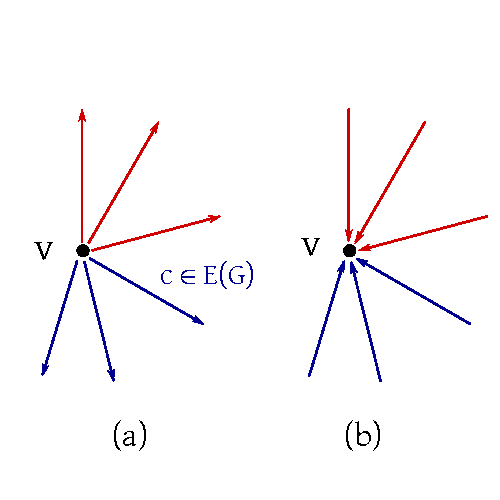
\includegraphics{img/proposition_5_1_proof.pdf}
    \caption{Proof for proposition 5.1}
   \end{center}
  \end{figure}

  (a) is $\delta^+_{\overleftrightarrow{G}}(v)$. (b) is $\delta^-_{\overleftrightarrow{G}}(v)$.

  \[
    \sum_{e \in \delta^+_G(v)} \underbrace{\left(\max\set{0, f' - f} - \max\set{0, f - f'}\right)}_{= f' - f} - \sum_{e \in \delta^-_G(v)} \left(f'(e) - f(e)\right)
  \] \[
      = \sum_{e \in \delta^+_G(v)} \left(f'(e) - f(e)\right) - \sum_{l \in \delta^-_G(v)} \left(f'(e) - f(e)\right)
      = 0
  \]

  2 cases for $e \in \overleftrightarrow{G} \setminus E(G_f)$:
  \[
    \begin{array}{llll}
      \text{forward edge} & e \in E(G) & f(e) = u(e) & g(e) = \max\set{0, f' - f} = \max\set{0, f' - u} = 0 \\
      \text{backwards edge} & \overleftarrow{e} \in E(G) & f(\overleftarrow{e}) = 0 & g(e) - \max\set{0, f - f'} = \max\set{0, 0 - f'} = 0
    \end{array}
  \]
\end{proof}

\begin{equation*}
  c(g) = \sum_{e \in \overleftrightarrow{E}(G)} g(e) c(e)
\end{equation*} \begin{equation*}
    = \sum_{e \in E(G)} c(e) \max\set{0, f'(e) - f(e)} + \sum_{\overleftarrow{e} \in E(G)} -c(\overleftarrow{e}) \max\set{0, f(\overleftarrow{e}) - f'(\overleftarrow{e})}
\end{equation*} \begin{equation*}
    = \sum_{e \in E(G)} c(e) \max\set{0, f' - f} + \sum_{e \in E(G)} c(e) [-\max\set{0, f - f'}]
\end{equation*} \begin{equation*}
    = \sum_{e \in E(G)} c(e) \underbrace{
      \left[\max\set{0, f'-f} - \max\set{0, f - f'} \right]
    }_{f'(e) - f(e)}
\end{equation*} \begin{equation*}
    = \sum_{e \in E(G)} c(e) \left(f'(e) - f(e)\right) = c(f') - c(f)
\end{equation*}

\begin{theorem}\label{proposition-5.2}
  For every circulation $f$ in a digraph $G$ there is a family $\mathcal{C}$ of at most $E(G)$ cycles in $G$ and positive numbers $h(C) \fall c \in \mathcal{C}$ with
  \[
    f(e) = \sum_{c \in \mathcal{C}, e \in E(C)} h(e)
  \]
\end{theorem}

\begin{proof}
  This follows directly from the flow decomposition theorem for \flow sts with arbitrary weighted $s,t \in V(G), s \neq t$ because circulation $f$ is also a \flow st with flow value $0$.
  \[
    f(e) = \sum_{P \in \mathcal{P}, e \in E(P)} h(P) + \sum_{c \in \mathcal{C}, e \in E} h(c)
      \fall e \in E(G), h(P) \geq 0 \fall P \in \mathcal{P}, h(C) \geq 0 \fall c \in \mathcal{C}
  \] \[
    \operatorname{value}(f) = \sum_{P \in \mathcal{P}} h(P) = 0 \Rightarrow h(P) = 0 \fall P \in \mathcal{P}
  \] \[
    \text{ with } \card{\mathcal{P}} + \card{\mathcal{C}} = \mathcal{O}(\card{E(G)})
  \]
\end{proof}

\begin{theorem}\label{satz-5.3}
  (Klein, 1967)
  Let $(G, u, b, c)$ be an instance of MKFP. A $b$-flow $g$ has minimum costs exactly iff there are no $f$-augmented cycles with negative costs in $G_f$.
\end{theorem}

\begin{proof}
  Direction of proof: $\Rightarrow$

  Assume that an $f$-augmented cycle $C$ (in $G_f$) exists with $\gamma < 0$ ($\gamma := \sum_{e \in E(C)} c_f(e)$). Let $\delta = \min_{e \in E(C)} u_f(e) > 0$.

  \begin{figure}[ht]
   \begin{center}
    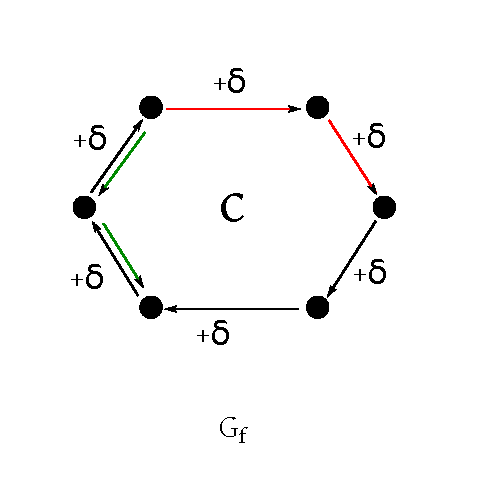
\includegraphics{img/satz_5_3.pdf}
    \caption{Proof of theorem~\ref{satz-5.3}}
   \end{center}
  \end{figure}

  Extension of $G_f$ from forward edge $\rightarrow +\delta$ in $G$. Backward edge from backward edge $\rightarrow -\delta$ in $G$.

  Augment flow and retrieve $f'$ with
  \[
    f \oplus c = f'(e) = \begin{cases}
      f(e)      & e \in E(C), \overleftarrow{e} \notin E(C) \\
      f(e) + \delta    & e \in E(C) \\
      f(e) - \delta    & \overleftarrow{e} \in E(C)
    \end{cases}
  \]
  $f'$ is a $b$-flow.

  \[
    c(f') = \sum_{e \in E(G)} c(e) f'(e) = \sum_{e \in E(G)} c(e) f(e) + \sum_{\overleftarrow, e \in E(C)} c(e)(f'(e) - f(e))
  \] \[
    = c(f) + \sum_{e \in E(C)} c(e) \delta + \sum_{e: \overleftarrow{e} \in E(C)} -c(e)(-\delta)
    = c(f) + \delta\left(\sum_{e \in E(C), e \in E(G)} c(e) - 2c(e)\right)
  \] \[
    e \in E(C), \overleftarrow{e} \notin E(C)
  \] \[
    = c(f) + \delta\left(\sum_{c \in E(C)} c(e) + \sum_{\overleftarrow{e} \in E(C)} c(\overleftarrow{e}) \right)
  \] \[
    c(f') = c(f) + \delta\gamma \Rightarrow c(f') \text{ is not optimal}
  \]

  Direction of proof: $\Leftarrow$

  Let $f$ be a not-minimum cost $b$-flow. Show that there exists some $f$-augmented cycle $K$ in $G_f$ with $c(k) < 0$.

  Let $f'$ be a $b$-flow with $c(f') < c(f)$.

  Definition as in Theorem~\ref{proposition-5.1}: $g: \overleftrightarrow{E} \rightarrow \mathbb{R}_+$ with $g(e) = \max\set{0, f' - f}$ and $g(\overleftarrow{e}) = \max\set{0, f - f'} \fall c \in E(G)$.

  According to Theorem~\ref{proposition-5.1}, $g$ is a circulation. From Theorem~\ref{proposition-5.2} it follows that family $\mathcal{C}$ of cycles in $\overleftrightarrow{E}$ exists with
  \[
    h: \mathcal{C} \rightarrow \mathbb{R}_+  \qquad G \mapsto h(C)
  \] \[
    g(e) = \sum_{c \in \mathcal{C}, e \in E(C)} h(c)
  \]

  Because $g(e) = 0 \fall e \notin G_f$, for all $c \in \mathcal{C}$ it holds that $E(C) \subseteq E(G_f)$ (Theorem~\ref{proposition-5.1}). Also it follows that $c(g) = c(f') - c(f) < 0$.

  \[
    0 > c(g)
      = \sum_{e \in \overleftrightarrow{E}(G)} c(e) g(e)
      = \sum_{e \in \overleftrightarrow{E}(G)} c(e) \sum_{C \in \mathcal{C}, e \in E(C)} h(c)
  \] \[
      = \sum_{C \in \mathcal{C}} h(c) \sum_{l \in \overleftrightarrow{E}(G) \cap E(G)} c(e)
      = \sum_{C \in \mathcal{C}} h(C)
  \] \[
    \Rightarrow \exists C \in \mathcal{C} \text{ with } c(C) < 0
  \]
\end{proof}

\subsection{Minimum-mean cycle cancelling algorithm}

\begin{algorithm}
  \caption{Minimum-mean cycle cancelling algorithm}
  \label{minimum-mean-cancelling-algo}
  \given{digraph $G$, $u: E(G) \rightarrow \mathbb{R}_+$, $c: E(G) \rightarrow \mathbb{R}$, $b: V(G) \rightarrow \mathbb{R}$ with $\sum_{v \in V(G)} b(v) = 0$}
  \find{A $b$-flow $f^*$ with minimum costs $c(f^*) = \sum_{e \in E(G)} c(e) \cdot f^*(c)$ or ``no $b$-flow exists in $G$''}
  \textbf{Remark.} $f'|_{E(G)}$ denotes $f'$ restricted to the edges $E(G)$ \par
\begin{algorithmic}[1]
  \State Extend $G$ by vertices $s,t$ and edges $(s, v)$, $(v, t) \fall v \in V(G)$ with $u((s,v)) = \max\set{0,b(v)}$. $u(v, t) = \max\set{0, -b(v)} \fall v \in V(G)$. Let $G'$ be an extended network. Determine max-$s$-$t$-flow $f'$ in $G'$.
  \If {$\operatorname{value}(f') < \sum_{v \in V(G)} b(v)$}
    \State ``there does not exist a $b$-flow in $G$''
  \Else
    \State let $f = f'|_{E(G)}$
  \EndIf
  \While{$\exists$ cycle with negative weights in $G_f$}
    \State Determine cycle $K$ with $\min\frac{c(K)}{\card{E(K)}}$ in $G_f$.
    \State Augment $f$ along $K: f := f \oplus K$
  \EndWhile
  \State \Return{$f$}
\end{algorithmic}
\end{algorithm}

\dateref{18th of November 2014}

\begin{theorem}
  (Corollary.)
  A $b$-flow has minimum costs iff $(G_f, C_f)$ has a (valid) potential function.
\end{theorem}
\begin{proof}
  $b$-flow $f$ is optimal $\Leftrightarrow$ $\nexists$ cycle $K$ with $c_f(K) < 0$ in $(G_f, C_f)$
  $\Leftrightarrow$ $\exists$ potential function $\pi: V(G_f) \rightarrow \mathbb{R}$ such that $c_f(n,f) + \pi(n) - \pi(v) \geq 0 \fall (u,v) \in E(G_f)$
\end{proof}

\begin{proof}
  Second proof to prove corollary (using linear programming)

  Let $(x_e)_{e \in E(G)}$ which corresponds to a $b$-flow. Costs:
  \[
    -\sum_{e \in E(G)} c_e x_e \rightarrow \text{ max}
  \] \[
    \text{Linear programming:}
      \sum_{e \in \delta^+(v)} x_e - \sum_{e \in \delta^-(v)} x_e = b(v) \fall v \in V(G)
  \] \[
    x_e \leq u_e \fall e \in E(G)
  \] \[
    x_e \geq 0 \fall e \in E(G)
  \]

  Dual problem:
  \[
    (DLP) \min{\sum_{v \in V(G)} b(v) y_v + \sum_{e \in E(G)} u_e z_e}
  \] \[
    y_u - y_v + z_e \geq - c_e \fall e = (u,v) \in E(G)
  \] \[
    z \geq 0 \fall e \in E(G)
  \] \[
    y_v \in \mathbb{R} \fall v \in V(G)
  \]

  Let $(x_e)_{e \in E(G)}$ be a $b$-flow.
  \[ \Rightarrow (x_e)_{e \in E(G)} \text{ is valid for linear programming} \]

  Theorem about complementary slacks:
  \begin{theorem}
    $x$ \text{ optimal} $\Rightarrow \exists$ optimal solution $(2_e)_{e \in E(G)}, (y_v)_v \in V(G)$
    of DLP with non-satisfied complementary slack.
  \end{theorem}

  \[
    \Rightarrow X_e(Y_u - Y_v + z_e + c_e) = 0 \fall e \in E(G)
  \] \[
    z_e (u_e - x_e) = 0 \fall e \in E(G)
  \]

  \[
    0 \leq -z_e \leq c(e) + y_u - y_v \text{ for } e = (u,v) \in E(G) \text{ with } X(e) < u(e)
  \] and \[
    c(e) + y_u - y_v = -z_e \leq 0 \text{ for } e = (u,v) \in E(G) \text{ with } X_e > 0
  \] \[
    \Rightarrow (y_v)_{v \in V(G)} \text{ is a potential function}
  \]

  because $c(u,v) + y_u - y_v \geq 0 \fall (u,v) \in E(G_f)$.
  We have 2 cases for $(u,v) \in E(G_f)$:
  \begin{enumerate}
    \item $x_{uv} < u_{uv}$ ($e = (u,v) \in E(G)$)
    \item $x_{uv} > 0$
  \end{enumerate}

  \[
    -c(u,v) + y_v - y_u \geq 0 \text{ from } c_e + y_u - y_v \leq 0
  \]
  Can all be inverted!
\end{proof}

\subsubsection[Analysis of MMCC]{Analysis of MMCC (Min Mean Cycle Cancelling algorithm)}
%
Denote the minimum average weight of a cycle in $G_f$ with $\mu(f)$
\[
  \mu(f) := \min_{k \text{ is cycle in } G_f} \frac{\sum_{e \in E(K)} c_f(e)}{\card{E(K)}}
\]

\begin{theorem}\label{lemma-5.5}
  Let $f_1, f_2, \ldots, f_K$ be a sequence of $b$-flows such that for all $i = 1, 2, \ldots, k-1$:
  $\mu(f_i) < 0$  and $f_{i+1}$ originates from $f_i$ by augmenting $f_i$ along cycle $K_i$ in $G_{f_i}$ ($f_{i+1} = f_i \oplus K_i$).

  For now let $K_i$ be a cycle with minimum average weight in $G_f$. Then the following statements hold:
  \[ \mu(f_i) \leq \mu(f_{i+1}) \fall i \]
  \[ \mu(f_i) \leq \frac{n}{n-2} \mu(f_c) \fall i < l \]
  with property that $K_i \cup K_l$ contains at least one pair of edges of opposing direction.
\end{theorem}

\begin{proof}
  Let $i$ be static. Consider $(V(G), E(K_i) \cup E(K_{i+1})$ and remove edges of opposing direction.
  Results in a digraph $H$ (edges occuring multiple times are counted twice).

  $H$ is subgraph of $G_f: (e \in E(K_{i+1}) \setminus E(G_f) \Rightarrow \overleftarrow{e} \in E(K_i))$.
  $H$ is Eulerian graph $\Rightarrow$ can be decomposed into several cycles $\overline{k_1}, \overline{k_2}, \ldots, \overline{k_e}$ in $G_{f_i}$.

  \begin{figure}[ht]
   \begin{center}
    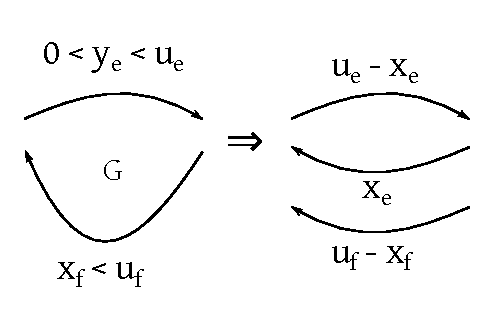
\includegraphics{img/lemma_5_5.pdf}
    \caption{Proof of theorem~\ref{lemma-5.5}}
   \end{center}
  \end{figure}

  \[ \frac{c(\overline{K_j})}{\card{E(K_j)}} \geq \mu(f_i) \fall 1 \leq j \leq l \]
  \begin{itemize}
    \item Equation 1:
      $\card{E(H)} = \sum_{j=1}^l \card{E(\overline{K_j})}$
    \item Weights of edges of opposing direction would cancel out each other:
      \[ c(E(H)) = \sum_{j=1}^l c(E(\overline{K_j}))
        \geq \sum_{j=1}^l \mu(f_i) \card{E(\overline{K_j})} = \mu(f) \card{E(H)} \]
      Equation 2:
      \[ c(E(H)) = c(E(K_i)) + c(E(K_{j})) = \mu(f_i) \card{E(K_i)} + \mu(f_{i+1}) \card{E(K_{i+1})} \]
  \end{itemize}
  From both equations it follows that
  \[
    \rightarrow c(E(H))
      \stackrel{\text{Equation 2}}{=} \mu(f_i) \card{E(K_i)} + \mu(f_i) \card{E(K_{i+1})}
      \stackrel{\text{Equation 1}}{\geq} \mu(f_i) \card{E(H)}
  \] \[
      \geq \mu(f_i) \card{E(K_i)} + \mu(f_{i+1}) \card{E(K_{i+1})}
  \]

  How can we show the last inequality $\geq$?
  \[
    \card{E(H)} \leq \card{E(K_i)} + \card{E(K_{i+1})} \qquad \mu(f_i) < 0 \text{ holds otherwise algorithm terminates}
  \] \[
    \mu(f_i) \card{E(H)} \geq \mu(f_i) \card{E(K_i)} + \mu(f_i) \card{E(K_{i+1})}
  \] \[
    \Rightarrow \mu(f_i) \leq \mu(f_{i+1})
  \]

  Proving point (2) of Theorem~\ref{lemma-5.5}: Consider without loss of generality $i,j$ such that $\mu(f_i) \leq \frac{n}{n-2} \mu(f_e)$ and $K_e$ and $K_j$ have no edges of opposing direction $\fall i < j < l$.

  Build $H$ from $(V(G), E(K_i) \cup E(K_e))$ by removal of opposing edges.

  $H$ is subgraph $G_{f_i}$
  \[ e \in E(K_l) \setminus G_{f_i} \Rightarrow \overleftarrow{e} \in E(K_i) \cup E(K_{i-1}) \cup \ldots \cup E(K_{l-1}) \Rightarrow \overleftarrow{e} \in E(K_i) \Rightarrow e \in E(H) \]
  This is a contradiction.

  Eulerian $H$ is decomposed into $\overline{K_1}, \ldots, \overline{K_t}$ cycles in $G_{f_i}$.
  Analogously as in point (1):
  \[ c(E(H)) \geq u(f) \card{E(H)}, c(E(H)) = \mu(f_i) \card{E(K_i)} + \mu(f_e) \card{E(K_l)} \]
  Furthermore it holds that
  \begin{align*}
    \card{E(H)}
      & \leq \card{E(K_i)} + \card{E(K_l)} - 2 \\
      & = \card{E(K_i)} + \card{E(K_l)} - \frac{2n}{n} \\
      & \leq \card{E(K_i)} + \card{E(K_l)} - \frac2n \card{E(K_e)} \qquad \text{ with } n \leq \card{E(K_e)} \\
  \end{align*}
  \[
    \Rightarrow E(H) \leq \card{E(K_i)} + \frac{n-2}{n} \card{E(K_e)}
  \]

  \[ \mu(f_i) \card{E(H_i)} \leq c(E(H_i)) = p(f_i) \card{E(K_i)} + \mu(f_e)\card{E(K_e)} \]
  \[ \mu(f_i) \card{E(K_i)} + \mu(f_i) \frac{n-2}{n} \card{E(K_2)} \]
  \[ \Rightarrow \mu(f_i) \leq \frac{n}{n-2} \mu(f_e) \]

  \begin{theorem}
    \textbf{(Corollary)}
    During the MMCC algorithm $\card{\mu(f)}$ is decremented all $m\cdot n$ iterations by at least factor $\frac12$.
  \end{theorem}
  \begin{proof}
    Let $K_i, K_{i+1}, \ldots, K_{i+m}$ be augmented cycles in $m$ continuous iterations of the algorithm.
    Every cycle has a bottleneck edge $\Rightarrow (n+1)$ bottleneck edges $\Rightarrow$ at least one repetition of an edge $\Rightarrow$ at least one pair $K_j, K_l$ exists for $i \leq j < l \leq i + m$ which contain edges of opposing direction. From Theorem~\ref{lemma-5.5} it follows that
    \[
      \mu(f_j) \leq \mu(f_j) \leq \frac{n}{n-2} \mu(f_e) \leq \frac{n}{n-2} \mu(f_{i+m})
    \] \[
      \card{\mu(f_i)} \geq \frac{n}{n-2} \card{\mu(f_{i+m})}
    \] \[
      \frac{n-2}{n} \card{\mu(f_i)} \geq \card{\mu(f_{i+m})}
    \]
    After $n$ such sequences of $m$ iterations (= after $n\cdot m$ iterations), $\mu(f)$ is decremented by at least $\left(\frac{n-2}{n}\right)^n < \frac{1}{e^2} < \frac12$.

    \[
      \card{\mu(f_{\text{new}})} \leq \left(\frac{n-2}{n}\right)^n \mu(f_{\text{old}}) < \frac12 \card{\mu(f_{\text{old}})}
    \]
  \end{proof}
\end{proof}

\begin{theorem}\label{proposition-5.6}
  Assume $c: E(G) \rightarrow Q$ (without loss of generality: $c: E(G) \rightarrow \mathbb{Z}$) it holds that:
  after $\mathcal{O}(nm \log_2{n} \card{c_{\text{min}}})$ iterations the MMCC algorithm terminates with
  $c_{\text{min}} = \min\set{\pm c_e | e \in E(G)}$.
\end{theorem}

\begin{proof}
  \textbf{Correctness.}
  Start with $b$-flow $f_0$:
  \[
    u(f_0) = \min_{K \text{ cycle in } G_{f_0}} \frac{\sum_{e \in E(K)} c(e)}{\card{E(K)}}
      \geq \min\frac{\card{E(K)} \cdot c_{\text{min}}}{\card{E(K)}}
  \] \[
    \mu(f_0) \geq c_{\text{min}}
  \] \[
    \card{\mu(f_0)} \leq \card{c_{\text{min}}}
  \]

  After $m\cdot n\cdot \log(n\card{C_{\text{min}}})$ iterations it holds that
  \[
    \card{\mu(f)}
      < {\frac12}^{\log_2{n\card{c_{\text{min}}}}} \card{\mu(f_0)}
      = \frac{1}{n\card{c_{\text{min}}}} \card{\mu(f_0)} \leq \frac1{n}
  \] \[
    \card{\mu(f)} < \frac1{n}
  \]

  Show that
  \[
    \card{\mu(f)} < \frac1{n} \Rightarrow \nexists \text{ negative cycle in } G_f
  \] \[
    \mu(f) = \frac{\sum_{e \in E(K^*)} c(e)}{\card{E(K^*)}} > -\frac1n
  \] \[
    \card{E(K^*)} \leq n \Rightarrow \frac{1}{\card{E(K^*)}} \geq \frac1n
  \] \[
    \mu(f) \leq \frac{\sum_{e \in E(K^*)} c(e)}{n}
      \text{ if } \sum_{e \in E(K^*)} c(e) < 0
  \] \[
    \Rightarrow \sum_{e \in E(K^*)} c(e)
      \geq n \cdot \mu(f)
      > n \left(-\frac1n\right) = -1
  \] \[
    \Rightarrow \sum_{e \in E(K^*)} c(e) > -1
  \] \[
    \text{ and } c(e) \in \mathbb{Z} \fall e \in E(G)
      \text{ where $K^*$ are cycles of minimum average weight}
  \] \[
    \Rightarrow \sum_{e \in E(K^*)} c(e) \geq 0
  \]
  This is a contradiction with $\sum_{e \in E(K^*)} c(e) < 0$.

  \textbf{Time complexity of MMCC.}
    $\mathcal{O}(mn)$ per iteration (determination of $K^*$ as optimal cycle)
    and $\mathcal{O}(nm\log{n} \card{C_{\text{min}}})$ iterations.
    \[ \Rightarrow \mathcal{O}(m^2 n^2 \log{n \card{c_{\text{min}}}}) \text{ runtime} \]
\end{proof}

\begin{theorem}\label{satz-5.7}
  (Tarjan, Goldberg, 1989)
  The MMCC algorithm can be implemented with $\mathcal{O}(m^3 n^2 \log{n})$ runtime.
\end{theorem}

\noproof{satz-5.7}

\dateref{24th of Nov 2014}

\section{Successive shortest path algorithm}

\begin{theorem}\label{satz-5.8}
  Let $(G, u, b, c)$ an instance of MKFP and $f$ be a $b$-flow with minimum costs.
  Let $P$ be a shortest \gath st in regards of $c_f$ in $G_f$ for any $s, t \in V(G_f)$.
  $f'$ results from $f$ by augmentation along $P$ by $\gamma \leq \min\set{u_f(e): e \in E(P)}$,
  hence
  \[
    f'(e) = \left\{\begin{array}{lc}
      f(e) & e \notin E(P), \overleftarrow{e} \notin E(P) \\
      f(e) + \gamma & e \in E(P) \\
      f(e) - \gamma & \overleftarrow{e} \in E(P)
    \end{array}\right\}
  \]

  Then $f'$ is a $b'$-flow with minimum costs where
  \[
    b'(v) = \left\{\begin{array}{lc}
      b(v) & \fall v \notin \set{s,t} \\
      b(v) + \gamma & v = s \\
      b(v) - \gamma & v = t
    \end{array}\right\}
  \]

  \begin{figure}[ht]
   \begin{center}
    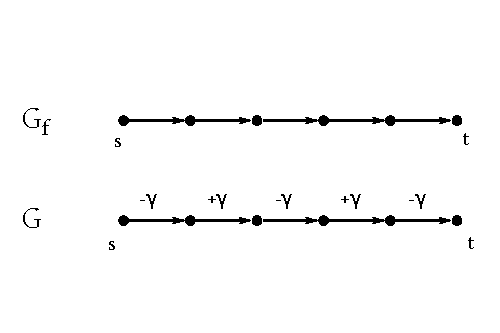
\includegraphics{img/satz_5_8.pdf}
    \caption{Proof of theorem~\ref{satz-5.8}}
   \end{center}
  \end{figure}
\end{theorem}

\begin{proof}
  Assume $f'$ is not a cost minimum $b'$-flow. So there exists a cycle $K$ with negative weights in $G_{f'}$.
  Consider $H_1 = \set{v(G), E(K) \cup E(P)}$. $H$ shall be derived from $H_1$ by removing any pairs of edges of opposing direction.

  \textbf{Observation.} $H$ is subgraph of $G_f$ because for $e \in E(K) \setminus E(G_f)$ it must hold that $\overleftarrow{e} \in E(G_f)$ and $(e, \overleftarrow{e})$ was already removed.
  \[ \Rightarrow \overleftarrow{e} \notin E(H) \]

  \begin{itemize}
    \item $c(E(H)) = c(E(K)) + c(E(P)) < c(E(P))$
    \item $\deg_H(v) \equiv 0 \mod{2}$ for $v \neq s, t$ (because of cycle and path).
  \end{itemize}

  $H$ can be decomposed into cycles $k_1, \ldots, k_l$ and a \gath st.

  \begin{figure}[ht]
   \begin{center}
    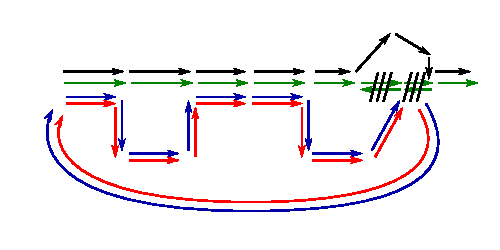
\includegraphics{img/satz_5_8_proof.pdf}
    \caption{Proof of theorem~\ref{satz-5.8} (cont.)}
   \end{center}
  \end{figure}

  \[ c(E(P_1)) \leq c(E(H)) = \underbrace{\sum_{i=1}^l c(E(K_i))}_{\geq 0} + c(E(P_1)) < c(E(P)) \]
  This is contradictory to the selection of $P$.
\end{proof}

\subsubsection{Initial flow for successively shortest path algorithm}
\begin{itemize}
  \item If $c$ is conservative, start with $0$-flow as optimal $b$-flow with $b=0$.
  \item If $c$ is not conservative, start with \[
      f(e) = \left\{\begin{array}{cc}
        u(e) & c(e) < 0 \\
        0    & c(e) \geq 0
      \end{array}\right.
    \]
    This is optimal for $b(v) = \sum_{\delta^+} f(e) - \sum_{\delta^-} f(e) \fall v \in V(G)$ because in $G_f$ it holds that $c_f(e) = c(\overleftarrow{e}) \geq 0 \fall e \in E(G_f)$ with $\overleftarrow{e} \in E(G)$ and $c(\overleftarrow{e}) \leq 0$ and $c_f(e) \geq 0 \fall e \in E(G_f)$ with $e \in E(G)$ and $c(e) = c_f(e) \geq 0$.
\end{itemize}

\subsection{Successively shortest path algorithm}
%
\begin{algorithm}
  \caption{Successively shortest path algorithm}
  \label{succ-shortest-path-algo}
  \given{$(G, u, b, c)$ network with $u: E(G) \rightarrow \mathbb{R}_+$ and $b: V(G) \rightarrow \mathbb{R}$ such that $\sum_{V(G)} b(v) = 0$. $c: E(G) \rightarrow \mathbb{R}$ is conservative}
  \find{Cost minimum $b$-flow $f$ or report ``there is no $b$-flow in $G$''}
\begin{algorithmic}[1]
  \State Let $f(e) = 0 \quad \fall e \in E(G) \quad b'(v) = b(v) \fall v \in V(G)$
  % step 2
    \If{$b'(v) = 0 \fall v \in V(G)$}\label{ssp-algo-step-2}
      \State stop and return $f$
    \Else
      \State chose $s \in V(G)$ with $b'(s) > 0$ and $t$ with $b'(t) < 0$, which is reachable from $s$ in $G_f$.
      \If{there does not exist $s, t$}
        \State stop and report there does not exist a $b$-flow in $G$.
      \EndIf
    \EndIf
  \State Determine a shortest \gath st $P$ in $G_f$ (shortest path in regards of weights $c_f$).
  \State Compute $\gamma = \min\set{b'(s), u_f(e) \fall e \in P, -b'(t)}$ (we are not allowed to overwrite $b'$s).
  \State Let $b'(s) = b'(s) - \gamma$ and $b'(t) = b'(t) + \gamma$.
  \State Augment $f$ along $P$: $f = f \oplus P$ (with value $\gamma$).
  \Goto{ssp-algo-step-2}
\end{algorithmic}
\end{algorithm}

\begin{theorem}\label{lemma-5.10}
  Let $G$ be a digraph with $u: E(G) \rightarrow \mathbb{R}_+$ and $b: V(G) \rightarrow \mathbb{R}$
  \[ \sum_{v \in V(G)} b(v) = 0 \]
  \begin{equation*}
    \exists \text{ $b$-flow in } G \Leftrightarrow \forall X \subseteq V(G) \text{ it holds that:}
  \end{equation*} \begin{equation*}
    \sum_{e \in \delta^+(X)} u(e) \geq \sum_{v \in V(X)} b(v)
  \end{equation*}
\end{theorem}

The proof for Theorem~\ref{lemma-5.10} is given in the practicals.

\begin{theorem}\label{proposition-5.9}
  If the algorithm terminates with ``there does not exist a $b$-flow in $G$'',
  this statement is correct.
\end{theorem}

\begin{proof}
  Let $X \subseteq V(G)$ such that $\forall v \in X$ it holds that,
  $v$ is reachable from $s$ in $G_f$,
  where $f$ is the current flow resulting in ``there does not exist a $b$-flow in $G$''
  and $s \in V(G)$ is a vertex with $b(s) > 0$ for which no $t \in V(G)$ with $b(t) < 0$
  reachable from $s$ in $G_f$ exists.

  \begin{figure}[ht]
   \begin{center}
    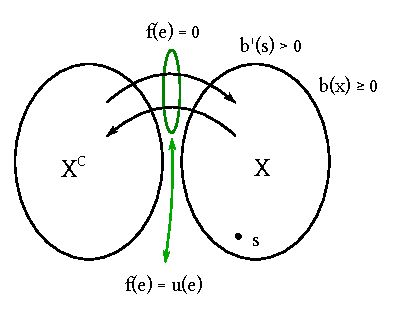
\includegraphics{img/proposition_5_9_proof.pdf}
    \caption{Proof of theorem~\ref{proposition-5.9}}
   \end{center}
  \end{figure}

  Then:
  \[ b'(v) \geq 0 \fall v \in X \text{ (otherwise we would have found some $t$)} \]
  \[
    \sum_{e \in \delta^+(X)} u(e)
      \subset
        \sum_{e \in \delta^+(X)} f(e)
        + \underbrace{\sum_{e \in X \times{} X \cap E(G)}}_{\text{all edges in } X}
        - \sum_{e \in X \times{} X \cap E(G)} f(e)
  \] \[
    = \sum_{v \in X} \left(\sum_{e \in \delta^+(v)} f(e) - \sum_{e \in \delta^-(v)} f(e) \right)
  \] \[
    = \sum_{x \in X} b(v) - b'(v) < \sum_{v \in X} b(v)
  \]
  because $b(v) - b'(v) \leq 0$ and one of them is smaller, because otherwise the algorithm would have terminated.
  $f$ is a $b''$ flow where $b - b'' = b'$.

  \[ \sum u(e) < \sum b(v) \]
  is a contradiction.

  From Theorem~\ref{lemma-5.10} it follows then that no $b$-flow exists.

  Does the algorithm terminate?
  Given $b(v) \in \mathbb{Z} \fall v \in V(G)$ and $u: E(G) \rightarrow \mathbb{Z}_+$ with the initial flow using integers. Then it holds that $b' \in \mathbb{Z}^{\card{V(G)}}$, $u_f \in \mathbb{Z}_+^{\card{E(G)}}$ and $y \in \mathbb{Z}_{*+}$ during the algorithm run.
  \[ \mathbb{Z}_{*+} = \set{1, 2, 3, \ldots} \]

  After each iteration:
  \[
    \underbrace{\sum_{v \in V(G)} \card{b_{\text{new}}'(v)}}_{\text{before augm.}}
      = \underbrace{\sum_{v \in V(G)} \card{b_{\text{old}}'(v)} - 2y}_{\text{after augm.}}
      \leq \sum_{v \in V(G)} \card{b'(v)} - 2
  \] \[
    \text{after at most } \frac12 \sum_{v \in V(G)} \sum \card{b(v)}
    \text{ iterations, it holds that } b' = 0
  \] \[
    B := \frac12 \sum_{v \in V(G)} \card{b(v)}
  \]

  \textbf{Time complexity.}
    \[ \mathcal{O}(B \cdot m \cdot n) \]
    $B$ iterations, $\mathcal{O}(mn)$ per iteration
    $\Rightarrow$ pseudo-polynomial
\end{proof}

\begin{theorem}\label{satz-5.10}
  If $u: E(G) \rightarrow \mathbb{Z}_+, b: V(G) \rightarrow \mathbb{Z}$ and $c$ is conservative,
  the successive shortest path algorithm can be implemented in $\mathcal{O}(nm + B(m + n \log{n}))$.
\end{theorem}

\begin{proof}
  Assume wlog. there exists exactly one $v \in V(G): b(v) > 0$. Otherwise consider $G' = (V(G) \dotcup \set{s}, E(G) \dotcup \set{(s, v): v \in V(G), b(v) > 0})$.

  \begin{figure}[ht]
   \begin{center}
    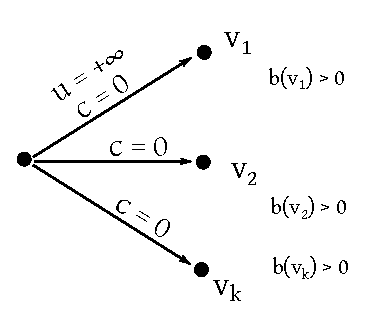
\includegraphics{img/satz_5_11.pdf}
    \caption{Proof of theorem~\ref{satz-5.10}}
   \end{center}
  \end{figure}

  \[
    \overline{b}(s) = \sum_{\substack{v \in V(G) \\ b(v) > 0}} b(v)
  \] \[
    \overline{b}(v) = \sum_{\substack{\forall v \in V(G) \\ b(v) > 0}} 0
  \]
  $\overline{b}(v) = b(v)$ for all other capacities $u$ of new edges. % that are large enough.

  Assumption wlog: All vertices $t$ with $b(t) < 0$ are only reachable from the single $s$ satisfying $b(s) > 0$. All vertices not reachable from $s$ and its incident edges can be removed.
\end{proof}

\begin{theorem}
  In every i-th iteration of the algorithm a potential function $\pi$ exists:
  \[
    \pi: V(G) \rightarrow \mathbb{R} \text{ in } G_{f_i}(c_{f_i}(u,v) + \pi(u) - \pi(v) \geq 0)
    \fall e \in E(G_{f_i})
  \]
\end{theorem}

\begin{proof}
  Proof by induction.

  \textbf{Induction base.} $f=0, c \text{ conservative}, G_{f_0} = G \Rightarrow \exists \text{ potential function $\pi_0$}$.

  \textbf{Induction step.}
  Let $f_{i-1}$ be a flow before the i-th iteration. From the induction hypothesis it follows that a potential function $\pi_{i-1}$ exists. The shortest path computation shall happen in regards of
  $c_{f_{i-1}}(u,v) + \pi_{i-1}(u) - \pi_{i-1}(v)$. Let $l_i(v)$ be the length of the shortest \gath sv in $G_{f_{i-1}}$.

  Let $\pi_i(v) = \pi_{i-1}(v) + l_i(v) \fall v \in V(G_{f_{i-1}})$. Show $\pi_i$ is a potential function in $G_{f_i}$.

  Consider $e = (x, y) \in E(G) \setminus E(P)$ (``old edges'')
  \[
    l_i(y) \leq l_i(x) + c_{\pi_{i-1}}(e) = l_i(x) + l(e) + \pi_{i-1}(x) - \pi_{i-1}(y)
  \] \[
    \Rightarrow 0 \leq c(e) + \pi_{i-1}(x) + l_i(x) - \left(\pi_{i-1}(y) + l_i(y)\right)
      = c(e) + \pi_i(x) - \pi_i(y)
  \]

  ``new edges'' or ``augmenting edges'': A new edge $\overleftarrow{e} = (y, x)$ is introduced on a path $P$ from $s$ to $t$ in a graph $G_{f_{i-1}}$ for some edge $(x, y)$. This new edge constitutes a new graph $G_{f_i}$.

  \[
    \fall e = (x, y) \in P \text{ it holds that }
      l_i(y) = l_i(x) + c_{\pi_{i-1}}(e) = l_i(x) + c(e) + \pi_{i-1}(x) - \pi_{i-1}(y)
  \] \[
    \Rightarrow 0 = c(e) + \pi_i(x) - \pi_i(y) \qquad \text{(analogously to ``old'' edges)}
  \] \[
    \Rightarrow c_{\pi_i}(\overleftarrow{e}) = -c_{\pi_i}(e) = 0
      \qquad \checkmark
  \]

  $\mathcal{O}(mn)$ in first iteration (first potential function).
  for other $\mathcal{O}(B)$ iterations, we use Dijkstra's algorithm to compute the shortest paths in $\mathcal{O}(m + n \log{n})$ per iteration and we compute the new potential function (as given in the induction step) in $\mathcal{O}(n)$
  \[ \Rightarrow{O}(mn + B(m + n \log{n})) \]
\end{proof}

\dateref{25th of Nov 2014}

\begin{algorithm}
  \caption{Capacity scaling algorithm}
  \label{min-b-flow-algo}
  \[ u(e) = +\infty \fall e \in E(G) \]
  \[ b(v) \in \mathbb{Z} \fall v \in V(G) \]
  \[ c: E(G) \rightarrow \mathbb{R} \text{ conservative} \]
  \given{$(G, c, b), \sum_{v \in V(G)} b(v) = 0, c$ conservative}
  \find{$b$-flow with minimum costs or $\nexists$ $b$-flow in $(G, c, b)$}
\begin{algorithmic}[1]
  \State $b'(v) := b(v) \fall v \in V$
  \State $f(e) := 0 \fall e \in E(G)$
  \If{$b_{\text{max}} > 0$}
    \State $y = 2^{\lfloor \log{b_{\text{max}}} \rfloor}$
      with ($b_{\text{max}} := \max\set{b(v) : v \in V(G)}$).
  \Else
     \State \Return{$f$}
  \EndIf
  \If{$b' = 0$ \label{cs-step-2}}
    \State \Return{$f$}
  \Else
    \State select vertex $s$ and $t$ with $b'(s) \geq \gamma$
    \State select vertex $b'(t) \leq -\gamma$ such that $t$ is reachable from $s$ in $G_f$.
    \If{no such pair exists}
      \State \Goto{cs-step-5}
    \EndIf
  \EndIf
  \State Determine a \gath st $P$ in $G_f$ with minimum weight (in regards of $c_f$).
  \State Let $b'(s) := b'(s) - \gamma$
  \State Let $b'(t) := b'(t) + \gamma$ (hence $\gamma$ flow units are going through $P$)
  \State $f := f \oplus P$
  \State \Goto{cs-step-2}
  \If{$y = 1$ \label{cs-step-5}}
    \Return{``no $b$-flow exists''}
  \Else{}
    \State $y := \frac{\gamma}{2}$
    \State \Goto{cs-step-2}
  \EndIf
\end{algorithmic}
\end{algorithm}

\begin{theorem}\label{satz-5.11}
  (Edmonds and Karp, 1972)
  The capacity scaling algorithm solves the MKFP with integers $b$, infinite capacities and conservative weights correctly. The algorithm can be implemented in $\mathcal{O}(n (m + n \log{n}) \log{b_{\text{max}}})$ runtime where $b_{\text{max}} := \max\set{b(v): v \in V(G)}$.
\end{theorem}

\begin{proof}
  \textbf{Correctness proof.}

  Analogously as with successively shortest paths (for $\gamma = 1$ we use integer integrity).
  So we have to point out that in step 4, the augmentation is valid.

  \begin{figure}[ht]
   \begin{center}
    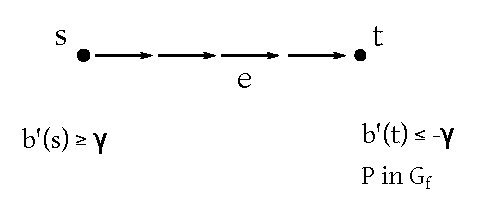
\includegraphics{img/capacity_scaling_algo_proof.pdf}
    \caption{Capacity scaling algorithm proof}
   \end{center}
  \end{figure}

  \textbf{Runtime complexity proof.}

  A \emph{phase} of the algorithm is a sequence of consecutive iterations which use the same value of $\gamma$. We prove: There are less than $4n$ augmentations in every phase.

  \textbf{Assumption.} There exists a phase with $\geq 4n$ augmentations. Let $f$ be a flow at the beginning of the phase. Let $g$ be a flow at the end of the phase.
  $g-f$ is a flow. Let $b''$ be balance values of $g-f$:
  \[
    b''(v) := \sum_{e \in \delta^+(v)} (g - f)(e) - \sum_{e \in \delta^-(v)} (g - f)(e)
  \]
  \clearpage
  \begin{itemize}
    \item It holds that $\sum_{v \in V(G)} \card{b''(v)} \geq 8n\gamma$.

      \textbf{Rationale.} $f, f_2, f_3, \ldots, f_l = g$

      \begin{figure}[ht]
       \begin{center}
        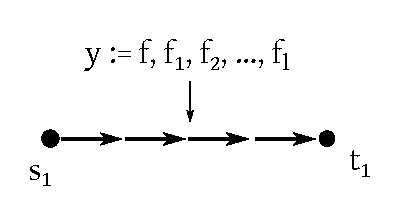
\includegraphics{img/capacity_scaling_algo_proof_rationale.pdf}
        \caption{Capacity scaling algorithm proof rationale}
       \end{center}
      \end{figure}

      \[ b_{f_1}(s_1) = b_{f}(s_1) + \gamma \]
      \[ b_{f_1}(v) = b_{f}(v) \fall v \in V(G) \setminus \set{t_1, t_2} \]
      \[ b_{f_1}(t_1) = b_{f}(t_1) - \gamma \]
      \[ \Rightarrow \sum_{v \in V(G)} \card{b_{f_1}(v)} = \sum_{v \in V(G)} \card{b_f(v)} + 2 \gamma \]

      After $\geq 4n$ iterations it holds that
      \[
        \sum_{v \in V(G)} \card{b_g(v)} \geq \sum_{v \in V(G)} \card{b_f(v)} + 8n\gamma
      \] \[
        \Rightarrow \sum_{v \in V(G)} \card{b''(v)} \geq 8n\gamma
      \]

    \item
      \begin{align*}
          S   &:= \set{x \in V(G): b''(x) > 0} \\
          S^+ &:= \set{x \in V(G): b''(x) \geq 2\gamma} \\
          T   &:= \set{x \in V(G): b''(x) < 0} \\
          T^+ &:= \set{x \in V(G): b''(x) \leq -2\gamma}
      \end{align*}

      Is there a path from $S^+$ to $T^+$ in $G_f$?
      No, otherwise the $2\gamma$ phase would not be finished yet.

      \begin{figure}[!ht]
        \begin{center}
          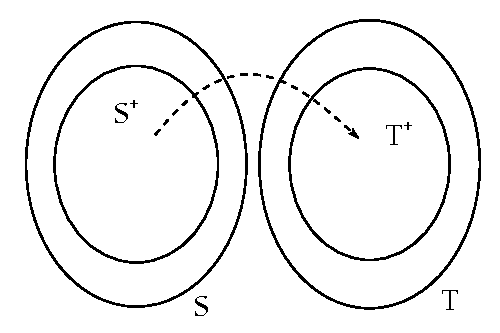
\includegraphics{img/capacity_scaling_algo_proof_sets.pdf}
          \caption{Capacity scaling algorithm: sets $S$, $S^+$, $T$ and $T^+$}
        \end{center}
      \end{figure}

      Let $\mathcal{X}$ be the set of reachable vertices from $S^+$ in $G_f$.
      $\Rightarrow$ the total value of all sinks reachable from $S^+$ is
      $\geq n (-2\gamma) = -2n\gamma$.

      In figure~\ref{fig:csa-xc}, if the upper edge does not exist, it is saturated,
      but $u(0) = \infty$ $\Rightarrow$ edge does not exist; analogously the other direction.

      Because g-f is a $b''$-flow, it holds that
      \[ \sum_{x \in S^+} b''(x) < 2n\gamma \]
      because in general it holds that
      \[ \sum_{x \in \mathcal{X}} b''(x) = 0 \]

      \begin{figure}[!ht]
        \begin{center}
          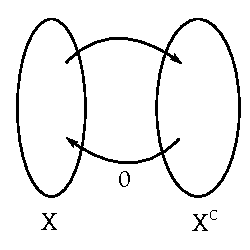
\includegraphics{img/capacity_scaling_algo_proof_edge.pdf}
          \caption{Capacity scaling algorithm: sets $X$ and $X^C$}
          \label{fig:csa-xc}
        \end{center}
      \end{figure}

      because
      \[
        0 = \sum_{v \in V(G)} b''(v)
          = \sum_{v \in \mathcal{X}} b''(v) + \sum_{v \in \mathcal{X}^C} b''(v)
          = \sum_{x \in \mathcal{X}} b''(v)
      \] \[
        = \sum_{v \in \mathcal{X}^C} \left(
          \sum_{e \in \delta^+(v)} \overline{f}(e) - \sum_{e \in \delta^-(v)} \overline{f}(e)
        \right)
        = \text{inner edges get cancelled} =
      \] \[
        = \sum_{e \in \delta^+(x^c)} \underbrace{f(e)}_{=0} + \sum_{e \in (\mathcal{X}' \times \mathcal{X}^C) \cap E(G)} f(e) - \sum_{e \in (\mathcal{X}^C \times \mathcal{X}^C) \cap E(G)} f(e) = 0
      \]

      \[
        \Rightarrow \sum_{v \in V(G)} \card{b''(v)}
          = 2\sum_{x \in S} b''(v)
          = 2\left(\sum_{x \in \delta^+} b''(v) + \sum_{x \in S \setminus S^+} b''(v)\right)
      \] \[
          < 2 (2n\gamma + 2n\gamma) = 8n\gamma
      \]
      This is a contradiction to our assumption.

      Hence there are $<4n$ augmentations per phase. The number of phases equals to the number of halvings of $2^{\lfloor \log{b_{\text{max}}}\rfloor}$ until $\gamma < 1$ is reached.
      \[ \Rightarrow \text{number of phases} \leq \log{b_{\text{max}}} + 1 \]
      \[ \Rightarrow \mathcal{O}(n \log{b_{\text{max}}}) \text{ iterations} \]
      with reduced costs from Theorem~\ref{lemma-5.10}
      \[ \mathcal{O}(mn + (m + n \log{n}) n \log{b_{\text{max}}}) \]
      \[ = \mathcal{O}((m + n \log{n}) n \log{b_{\text{max}}}) \]
  \end{itemize}

\end{proof}

\section{Time-dependent dynamic flow}
%
\dateref{1st of Dec 2014}
\begin{itemize}
  \item Transit time per edge
  \item Value of flow over edge $e$ can vary in time process
    \[ f_e(t) \qquad \text{flow values at timestamp $t$ at edge $e$} \]
\end{itemize}

\textbf{Definition.}
  Let $(G, u, s, t)$ be a network with capacities $u: E(G) \rightarrow \mathbb{R}_+$, source $s$, sink $t$ and transit times $l: E(G) \rightarrow \mathbb{R}_+$ ($e \mapsto l(e)$) and a time horizon $[0, T]$ with $T \in \mathbb{R}_+$. Then a timedependent \flow st $s$ is a Lebesgue-measurable function $f_e: [0, T] \rightarrow \mathbb{R}_+ \fall e \in E(G)$ with all properties:
  \begin{itemize}
    \item $f_e(\zeta) \leq u(e) \fall e \in E(G) \fall \zeta \in [0, T]$
    \item $\operatorname{ex}_f(v, a) :=
      \sum_{e \in \delta^-(v)} \int_0^{\max\set{0, a-l(e)}} f_e(\zeta) \,d\zeta
      - \sum_{e \in \delta^+(v)} \int_0^a f_e(\zeta) \, d\zeta \geq 0
      \fall v \in V(G) \setminus \set{s} \fall a \in [0, T]$
  \end{itemize}

$\operatorname{value}(f) := \operatorname{ex}_f(t, T)$ is called value of flow at timestamp $T$.

\subsection{Max-Flow-over-time problem (MFoTP)}
\given{$(G, u, s, t, l$), $T \in \mathbb{R}_+$}
\find{Determine a timedependent flow $f_e: [0, T] \rightarrow \mathbb{R}_+ \fall e \in E(\zeta)$ with maximum value $f$}

\begin{theorem}\label{satz-5.21}
  (Ford, Fulkerson, 1958)
  The MFoTP can be solved with the same time complexity like MKFP.
\end{theorem}

\begin{proof}
  MFoTP can be reduced to (static) MKFP.
  Without loss of generality: There are no edges ending in $s$ in $G$ (flow delay!).
  Construct a new network $(G', u, 0, c)$.
  \[ G' = (V(G), E(G) \cup \set{(t, s)}) \]
  \[ u: E(G') \rightarrow \mathbb{R}_+ \]
  with $u(e)$ as the same like in $(G, s, t, u, l)$ for $e \in E(G)$ and $u(t, s) = \sum_{e \in E(G)} u(e)$.
  \[ c: E(G') \rightarrow \mathbb{R} \]
  \[
    c(e) = \left\{\begin{array}{ll}
      l(e) & e \in E(G) \\
      -T & e = (t, s)
    \end{array}\right.
  \]

  Determine a circulation $f'$ with minimum costs in $(G', u, 0, c)$.

  \textbf{Theorem of Gallai:} There exists a family $\mathcal{C}$ of cycles in $g'$ with $h: \mathcal{C} \rightarrow \mathbb{R}_{+*}$, $K \mapsto h(K) > 0$ with $\card{\mathcal{C}} = \mathcal{O}(\card{E(G')})$ and $f(e) = \sum_{K \in \mathcal{C}, e \in K} h(K) \fall e \in E(G')$.

  $f'$ has minimum costs $\rightarrow$ $c(K) \leq 0 \fall K \in \mathcal{C}$.

  In the other case if $K_*$ with $c(K_*) > 0$ exists, consider $f''$ with $f''(e) = \sum_{K \in \mathcal{C} \setminus \set{K_*}, e \in K} h(K) \fall e \in E(G')$. $f''$ is circulation.

  \[
    c(f'') = \sum_{e \in E(G')} f''(e) \cdot c(e)
      = \sum_{K \in \mathcal{C} \setminus \set{K_*}} c(K)
      < \sum_{K \in \mathcal{C}} c(K)
      = c(f')
  \]
  This would be a contradiction.

  \[
    (t, s) \in K \fall K \in \mathcal{C} \text{ because $(t, s)$ is the only edge with negative costs}
  \]
  Let $e = (v, w) \in K$. Denote $d_e^K$ the length of the path of $s$ to $v$ in $K$ in regards of costs $c$. Define
  \[
    f_e^*(\zeta) =
      \sum_{\substack{
        k \in \mathcal{C}, c(K) < 0 \\
        e \in K, d_e^K \leq \zeta \leq d_e^K - c(K) \\
        \zeta \leq T - l(e) - d_{w,t}^K \\
        d_{w,t}^K + \zeta + l(e) \leq T}}
      h(K)
      \fall e \in E(G) \fall 0 \leq \zeta \leq T
  \]

  Define
  \[ c(k) = d_e^K + l(e) + d_{w,t}^K - T \]
  \[ d_e^K - c(K) = T - l(e) - d_{w,t}^K \]

  When is $s_0$ a $f_e^*(\zeta)$ dynamic flow?
  \begin{equation}
    f_e^*(\zeta) = \sum h(K) \leq \sum_{\substack{K \in \mathcal{C} \\ c(K) < 0 \\ e \in K}} h(K) = f'(e) \leq n(e) \fall e \fall \zeta \in [0, T]
  \end{equation} \begin{equation}
    \operatorname{ex}_f(v, a) = \sum_{e \in \delta^-} \int_0^{\max\set{0, a-l(e)}} \dots
      - \sum_{e \in \delta\dots} \int_0^a \dots \stackrel{!}{\geq} 0 \\
  \end{equation} \begin{equation*}
    \sum_{e \in \delta^-(v)} \sum_{\substack{K \in \mathcal{C} \\ c(K) < 0 \\ e \in K}} h(K)
      - \sum_{e \in \delta^+(v)} \sum_{\substack{K \in \mathcal{C} \\ c(K) < 0 \\ e \in K}} h(K)
      = \sum_{e \in \delta^-(v)} f'(e) - \sum_{e \in \delta^+(v)} f'(e) = 0
  \end{equation*}
  because $f'$ is circulation
  \begin{equation*}
    \operatorname{value}(f^*)
      = \operatorname{ex}_{f^*}(t, T)
      = \underbrace{\sum_{e \in \delta^-(t)} \int_0^{\max\set{0, T - l(e)}} f_e^K(\zeta) \,d\zeta}_{A}
      \stackrel{!}{=} -\sum_{e \in E(G')} c(e) f'(e)
  \end{equation*}
  \begin{equation*}
    A = \sum_{e \in \delta^-(t)} \int_0^{\max\set{0, T - l(e)}}
      \sum_{\substack{K \in \mathcal{C} \\ c(K) < 0 \\ e \in K \\ d_e^K \leq \zeta \leq d_e^K - c(K)}}
      h(K) \,  d\zeta
  \end{equation*} \begin{equation*}
      = \sum_{e \in \delta^-(t)} \sum_{\substack{K \in \mathcal{C} \\ c(K) < 0 \\ e \in K}} h(K) \int_{d_e^K}^{d_e^K -c(K)} 1 \,d\zeta
      = \sum_{e \in \delta^-(t)} \sum_{\substack{K \in \mathcal{C} \\ c(K) < 0 \\ e \in K}} h(K) (-c(K))
  \end{equation*} \begin{equation*}
      = \sum_{e \in \delta^-(t)} \sum_{\substack{K \in \mathcal{C} \\ c(K) < 0 \\ e \in K}} h(K) \left(
        -\sum_{e \in K} l(e) + T
      \right)
  \end{equation*} \begin{equation*}
    = \sum_{e \in E(G)} -l(e) \underbrace{\sum_{\substack{K \in \mathcal{C} \\ c(K) < 0 \\ e \in K}}}_{f'(e)} h(K)
    + T \left(\sum_{e \in E(G)} f'(e) - \sum_{e \in E(G)} f'(e)\right)
  \end{equation*} \begin{equation*}
    = \sum_{e \in E(G)} -l(e) f'(e)
  \end{equation*}
\end{proof}

\section{Matchings}
%
\subsection{Definitions and optimality criterion}
%
\index{Matching}
\index{Matched vertex}
\index{Perfect matching}
\index{Maximal matching}
\index{Matching number}
\index{Vertex}
\index{Minimum vertex cover}
\index{Vertex cover number}
\begin{definition}
  $G = (V, E)$ is undirected.
  $M \subseteq E$ is called \emph{matching} if $\fall e_1, e_2 \in M: e_1 \cap e_2 = \emptyset$ (in words: no edges share a vertex).
  A vertex $v$ is \emph{matched by $M$} if $\exists e \in M$ with $v \in e$.
  A matching $M$ is called \emph{perfect} if every vertex of $M$ is matched by $M$.
  A matching $M$ is called \emph{maximal} if for every matching $M'$, $\card{M'} \leq \card{M}$.
  The \emph{matching number of $G$} is defined as
  \[ \mathfrak V(G) \coloneqq \max\set{\card{M}: M \text{ is a matching}} \]
  A \emph{vertex cover} is a subset $C \subseteq V(G)$ such that $e \cap C \neq \diameter \fall e \in E(G)$.
  A \emph{minimum vertex cover} is a vertex cover of minimum cardinality.
  The \emph{vertex cover number of $G$} is defined as
  \[ \mathfrak C(G) \coloneqq \min\set{\card{C}: C \text{ is vertex cover}} \]
\end{definition}
%
\begin{observation}
  For a triangle (3 vertices, 3 edges):
  \[ \mathfrak C(K_3) = 2 \qquad \mathfrak V(K_3) = 1 \]
\end{observation}
\begin{theorem}
  Let $M$ is a matching. Let $C$ is a vertex cover. It holds that,
  \[
    \mathfrak V(G)
      = \max_{\text{$M$ matching}} \card{M}
      \leq \min_{\text{$C$ vertex cover}} \card{C}
      = \mathfrak C(G)
  \] \[
    \Rightarrow \mathfrak V(G) \leq \mathfrak C(G)
  \]
\end{theorem}

\index{Alternating path (matchings)}
\begin{definition}
  Let $G$ be an undirected graph and $M$ a matching. A path in $G$ is called $m$-alternating if its edges are alternatingly assigned to the matching and not assigned. Hence
  \[ P = (v_0, v_1, v_2, \ldots, v_k) \]
  \[
    (v_{i-1}, v_i) \in M \Rightarrow v_i, v_{i+1} \notin M \qquad\text{ and }
  \] \[
    (v_{i-1}, v_i) \notin M \Rightarrow v_i, v_{i+1} \in M \quad
    \fall 1 \leq i \leq k
  \]

  \index{Augmenting path (matchings)}
  If a $M$-alternating path starts and ends with a non-matched vertex, it is called $M$-augmenting.
  An example is given in figure~\ref{img:maugmenting}.
\end{definition}
%
\begin{figure}[p]
  \begin{center}
    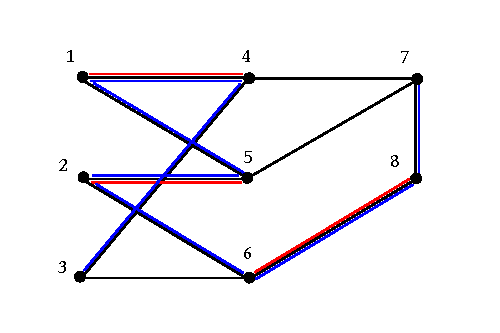
\includegraphics{img/M-augmenting_path_example.pdf}
    \caption{
      $M$-augmentating path example.
      Red edges define a matching, blue edges define an $m$-augmenting path from $3$ to $7$.
      $P = (3, 4, 1, 5, 2, 6, 8, 7)$.
    }
    \label{img:maugmenting}
  \end{center}
  \begin{center}
    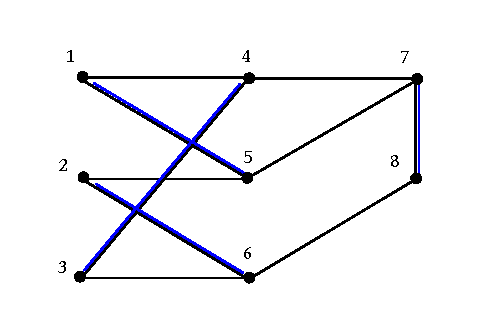
\includegraphics{img/Mprime_example.pdf}
    \caption{
      $M'$ of the $M$-augmentating path example.
      You can immediately recognize that it is indeed a matching
      and $\card{M} = 3$ whereas $\card{M'} = 4$.
    }
    \label{img:mprime}
  \end{center}
  \begin{center}
    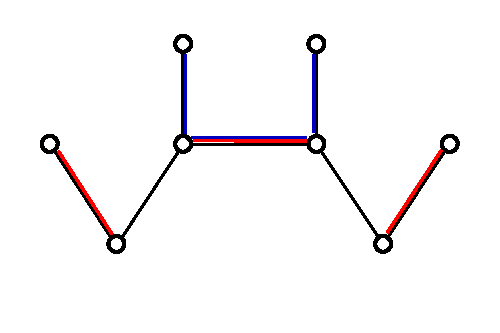
\includegraphics{img/M-augmenting_path_and_maximal.pdf}
    \caption{
      An $M$-augmenting path (blue) and a maximal matching (red).
      You can exchange $M \cap P$ with the edges of $M \triangle P$
      and will end up with a maximal matching.
    }
    \label{img:augmenting-and-maximal}
  \end{center}
\end{figure}
%
\begin{observation}
  Let $M' \coloneqq M \triangle P$ where $M$ is a matching and $P$ is an M-augmenting path:
  \[ M' = (M \setminus P) \cup (P \setminus M) \]
  \begin{itemize}
    \item We show: $M'$ is a matching (compare with figure~\ref{img:mprime}).
      Let $e_1, e_2 \in M'$
      \begin{itemize}
        \item $e_1, e_2 \in M \setminus P \Rightarrow e_1 \cap e_2 = \diameter$
        \item $e_1, e_2 \in P \setminus M \Rightarrow e_1 \cap e_2 = \diameter$
        \item $e_1 \in M \setminus P, e_2 \in P \setminus M \Rightarrow e_1 \cap e_2 = \diameter$
      \end{itemize}

    \item We show: $\card{M \cap P} = \card{P \setminus M} - 1$.

      It holds that, $\card{M'} = \card{M} + 1$, because $P$ contains one matching edge
      for one non-matching edge and one additional non-matching edge.
      \begin{align*}
               M' &= (M \setminus P) \cup (P \setminus M) \\
      \intertext{It is trivial to see that $(M \setminus P)$ and $(P \setminus M)$ are disjoint. Hence,}
        \card{M'} &= \card{M \setminus P} + \card{P \setminus M} \\
      \intertext{For any two sets $M$ and $P$ it holds,}
                M &= (M \cap P) \cup (M \setminus P) \\
      \intertext{Also $M \cap P$ and $M \setminus P$ are disjoint. Hence,}
         \card{M} &= \card{M \cap P} + \card{M \setminus P}
      \end{align*}
      Followingly,
      \begin{align*}
        \card{M} + 1 &= \card{M'} \\
        \card{M \cap P} + \card{M \setminus P} + 1 &= \card{M \setminus P} + \card{P \setminus M} \\
        \card{M \cap P} &= \card{P \setminus M} - 1
      \end{align*}
  \end{itemize}

  We conclude:
  \[
    \Rightarrow
    \underbrace{\card{M \cap P}}_{\text{red edges in figure~\ref{img:maugmenting}}} =
    \underbrace{\card{P \setminus M}}_{\text{blue edges in figure~\ref{img:mprime}}} - 1
  \]
  We call $P$ \emph{$M$-augmenting}.
\end{observation}

\dateref{2nd of Dec 2014}

\begin{theorem}[Berge, 1957]
  \label{satz-6.1}
  Let $M$ be a matching in $G$. $M$ is maximal if and only if there is no $M$-augmenting path in $G$.
\end{theorem}

\begin{proof}
  \begin{description}
    \item[Direction of proof: $\Leftarrow$] \hfill{} \\
      Proof by contradiction: Assume there exists a $M$-augmenting path. \\
      Then $M$ is not maximal (see section about max-flows)%
      \footnote{Informally put: make matched edges not matched, vice versa and you retrieve a larger matching.}.

    \item[Direction of proof: $\Rightarrow$] \hfill{} \\
      Proof by contradiction: Assume $M$ is not maximal and no $M$-augmenting path exists.

      \begin{enumerate}
        \item Then there exists a matching $M'$ such that $\card{M'} > \card{M}$.
        \item Consider $D = M \triangle M'$ (= $(M \setminus M') \cup (M' \setminus M)$).
          It holds that,
          \[ \deg_{D}(v) \leq 2  \quad \fall v \in V(G) \]
          because if more than three edges touch vertex, then edges in $M$ and $M'$ cannot be alternating.
        \item $D$ consists of the following components:
          \begin{itemize}
            \item Isolated vertices
            \item Cycles with alternating edges
            \item Paths with alternating edges with distinct end points
          \end{itemize}
          Cycles must have an even cardinality, because edges are alternating,
          because otherwise two edges of $M$ or $M'$ are not disjoint.
        \item $M'$ is larger than $M$ according to (1.), followingly one component
          of $D$ has more edges from $M'$ than $M$\footnote{
          The two vertices of the additional edge cannot occur in two different components,
          because edges are not included if they occur neither in $M$ nor $M'$ or in both.
          So if you start with a vertex matched only by $M'$ you get an alternating
          sequence of edges until you end up with another vertex only matched by $M'$.}
        \item This component cannot be an isolated vertex (no edges) or cycles
          with alternating edges (contradiction to even cardinality). So it must be
          a path. This path is alternating.
      \end{enumerate}
      This is a contradiction to our assumption, that no $M$-augmenting path exists.
  \end{description}
\end{proof}

\textbf{Algorithmic idea.}
  \begin{enumerate}
    \itemsep0pt
    \item Start with arbitrary matching $M = M_0$ (eg. $M_0 = \diameter$).
    \item While there exists an $M$-augmented path $P$, repeat
      \[ M := M \triangle P \]
    \item $M$ is maximal. Return $M$.
  \end{enumerate}

\subsection{Matchings in bipartite graphs}
%
\begin{theorem}
  \label{thm:bipartite-mmp-to-mfp}
  The $M \triangle P$ maximum matching problem (MMP) for bipartite graphs
  is a special case of the max-flow problem (MFP).
\end{theorem}
\begin{proof}
  Let $G = (A \dotcup B, E)$ be an undirected, bipartite graph.
  Let $(G', u, s, t)$ be a network where $G'$ is a digraph.
  \[ s, t \notin A \dotcup B \qquad s \neq t \]
  \[ V(E') = A \dotcup B \dotcup \set{s, t} \]
  \[ E(G') = \set{(s, a): a \in A} \cup \set{(b, t): b \in B} \dotcup \set{(a,b) \in E(G), a \in A, b \in B} \]

  \begin{figure}[ht]
   \begin{center}
    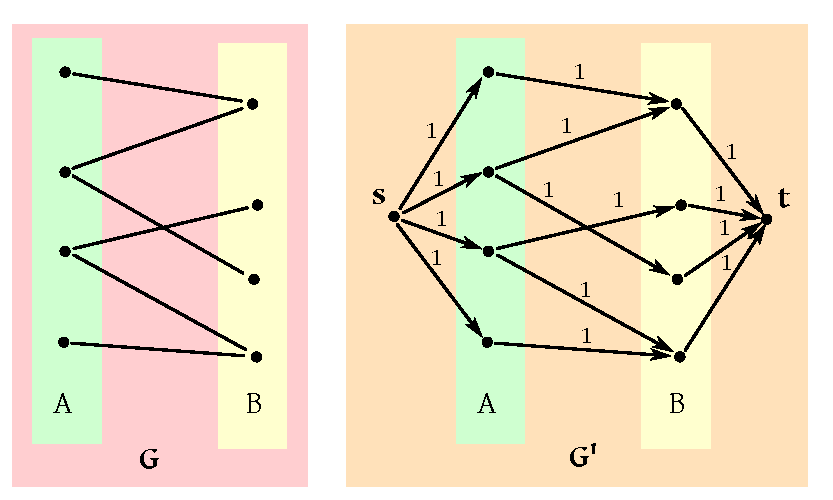
\includegraphics[width=\textwidth]{img/matching_bipartite.pdf}
    \caption{
      An example for a bipartite graph $G$ converted into a max-flow problem $(G', u, s, t)$.
      It is very interesting to recognize that the selection of vertices for set $A$ or $B$
      is irrelevant. So you can also make the flow go from right to left.
    }
    \label{img:bipartite-matching-to-network}
   \end{center}
  \end{figure}

  \begin{observation}
    \begin{itemize}
      \item Every matching $M$ in $G$ corresponds to a complete flow $F_M$ in $G'$.
      \item Every flow $f$ in $(G', u, s, t)$ corresponds to one matching $M_f$ in $G$.
    \end{itemize}
  \end{observation}

  How? We show those relations formally:
  \begin{itemize}
    \item Given a bipartite graph $G = (A \dot\cup B, E)$. Consider a flow $f_M$:
      \[
        f_M(e) = \begin{cases}
          1 & e = (a, b) \in A \times B, e \in M \\
          0 & e = (a, b) \in A \times B, e \notin M \\
          1 & e = (s, a), a \in A, \text{matched} \\
          0 & e = (s, a), a \in A, \text{unmatched} \\
          1 & e = (b, t), b \in B, \text{matched} \\
          0 & e = (b, t), b \in B, \text{unmatched} \\
        \end{cases}
      \] \[
        \operatorname{value}(f_M) =
          \sum_{a \in A} f(s, a)
      \] \[
          = \card{\set{a : a \in A, f(s, a) = 1}}
          = \card{\set{a : a \in A, a \text{ is matched}}} = \card{M}
      \]
    \item Let $f$ be a \flow st in $(G', u, s, t)$ with integer values 0 and 1.
      \[ \Rightarrow f(e) \in \set{0, 1} \fall e \in E(G') \]

      Consider $M_f \coloneqq \set{e \in A \times B: f(e) = 1}$.
      Claim: $M_f$ is matching.

      Proof by contradiction: Consider $e_1 = (a, b_1) \in M$ and $e_2 = (a, b_2) \in M$.
      In a matching no edges $e_1$ and $e_2$ exist which share a common vertex.
      So, this statement must turn out to be wrong.
      \begin{align*}
          \Rightarrow \sum_{e \in \delta^-(a)} f(e) &= f(s, a) = 1 \\
          \Rightarrow \sum_{e \in \delta^+(a)} f(e) &= f(e_1) + f(e_2) = 2
      \end{align*}
      This is a contradiction to the flow conservation condition. $f$ cannot be a flow,
      but we assumed that. So actually, no two edges $e_1$ and $e_2$ exist which share
      a common vertex.

      Analogously to the first observation, it holds that
      \[ \operatorname{value}(f) = \card{M_f}. \]
  \end{itemize}

  Given a bipartite graph $(A \dotcup B, E)$ and you want to determine a maximum matching.
  Then create one supersource and one supersink. Connect the supersource with all
  vertices of set $A$ and all vertices of set $B$ with the supersink. Every edge
  between $A$ and $B$ becomes a directed one from $A$ to $B$. Assign $1$ as capacity
  to all edges. The max-flow of this network $(G, u, s, t)$ yields a maximum matching.
  Figure~\ref{img:bipartite-matching-to-network} illustrates this construction.
\end{proof}

MMP in bipartite graphs is solvable with $\mathcal{O}(mn)$ runtime, eg. with Ford-Fulkerson
in $n$ iterations (flow extension by $1$ unit per iteration) and $\mathcal{O}(m)$ runtime
for determination of some \gath st in $G_f$.
\[ \mathfrak V(G) \leq \mathfrak C(G) \]
In bipartite graphs \emph{equivalence} holds (K\H{o}nig, 1937):

\begin{theorem}\label{satz-6.2_}
  Let $G = (V_1 \dotcup V_2, E)$ be a bipartite graph.
  Then it holds $\mathfrak V(G) = \mathfrak C(G)$.
\end{theorem}

\begin{proof}
  $\mathfrak V(G) \leq \mathfrak C(G)$ has been shown for general graphs.
  Show that $\mathfrak C(G) \geq \mathfrak V(G)$.

  Consider MMP as MFP (as in Figure~\ref{img:bipartite-matching-to-network}).
  Let $f$ be a maximum \flow st of integer values.
  Let $\delta(s)$ be the corresponding minimum cut.
  \[ u(\delta(s)) = \operatorname{value}(f) \]
  There does not exist $e \in (S \cap V_1) \times (S' \cap V_2)$.

  \textbf{Assumption.} There exists $e = (a, b)$. Case distinction:
  \begin{enumerate}
    \item $f(e) = 0 \Rightarrow e \in E(G_f) \Rightarrow b \in S$. This is a contradiction.
    \item $f(e) = 1 \Rightarrow \sum_{e \in \delta^-(a)} f(e) - \sum_{e \in \delta^+(a)} f(e) = 0$
      \[ f(s, a) = \sum_{e \in \delta^+(a)} f(e) \geq 1 \Rightarrow f(s, a) = 1 \]
  \end{enumerate}

  \begin{figure}[ht]
   \begin{center}
    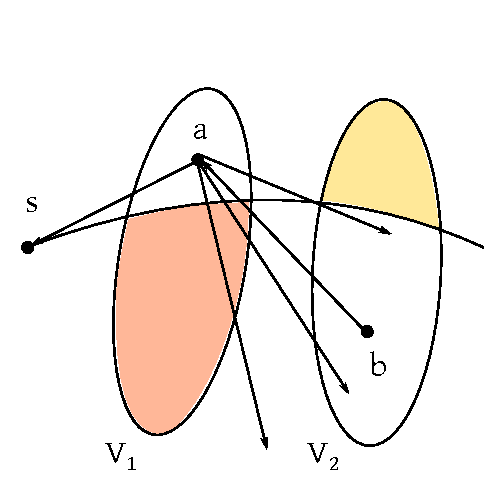
\includegraphics{img/bipartite_increment.pdf}
    \caption{Bipartite matching -- Residual graph}
   \end{center}
  \end{figure}

  Hence $a$ is only reachable from $b$. $b \notin S \Rightarrow a$ is not reachable. Contradiction.

  \[ \Rightarrow \nexists e \in (S \cap V_1) \times (S^C \times V_2) \]

  Construct cover: $C = (V_1 \cap S^C) \cup (V_2 \cap S)$.

  Compare $\operatorname{value}(f)$ and
  \[
    \card{c}
      = \card{V_1 \cap S^C} + \card{V_2 \cap S}
      = \card{V_1 \cap S^C} + \set{(a, t): a \in S}
  \] \[
    \operatorname{value}(f) = u(\delta(s)) = \sum_{e \in \delta^+(\mathcal{S})} u(e)
      = \card{\delta^+(\mathcal{S})}
      \stackrel{!}{=} \card{S^C \cap V_1} + \card{S \cap V_2}
  \]
\end{proof}

\begin{figure}[ht]
 \begin{center}
  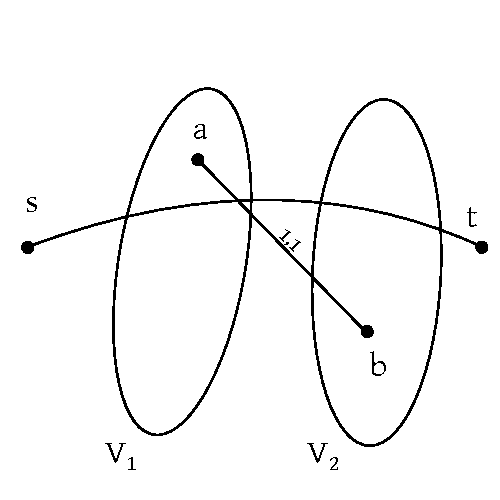
\includegraphics{img/bipartite.pdf}
  \caption{Bipartite graph}
 \end{center}
\end{figure}

\begin{theorem}[Hall's marriage condition]
  \label{satz-6.3}
  Let $G$ be a bipartite graph $(A \dotcup B, E)$ then $G$ has a covering matching for $A$ if and only if $\card{\Gamma(X)} \geq \card{X} \fall X \subseteq A$ where $\Gamma(X) = \set{b \in B: \exists a \in X, (a, b) \in E(G)}$.
\end{theorem}

\begin{theorem}[Marriage corollary]
  \label{marriage-corollary}
  Let $G$ be a bipartite graph with $V(e) = A \dotcup B$ and $\card{A} = \card{B}$.
  $G$ has a perfect matching if and only if $\fall X \subseteq A$ with $\card{\Gamma(X)} \geq \card{X}$ holds.
\end{theorem}

\subsection{Theorem of Tutte}
%
Consider \emph{general} graphs again.
Let $X \subseteq V(G)$. We define\footnote{In words:
$X$ and all incident edges with $X$ are removed from the graph $G$}:
\[
  G \setminus X \coloneqq
  (V \setminus X, \set{(u, v) \in E \,\middle|\, u \not\in X \land v \not\in X}).
\]

\index{$q_G(X)$}
Let $q_G(X)$ be the number of even (in terms of number of vertices) connected components in $G \setminus X$.
Then we can observe: $q_G(X) > \card{X} \Rightarrow \nexists$ perfect matching in $G$.
\[
  \Rightarrow
    \underbrace{
      q_G(X) \leq \card{X} \fall X \subseteq V(G)
    }_{\text{Tutte condition}}
\]
\begin{center}
  \dots{} is necessary and sufficient for existence of a perfect matching in $G$
\end{center}

\textbf{Definition.}
  \index{factor-critical graphs}
  \index{almost perfect matching}
  A graph $G$ is called \emph{factor-critical}, if $G \setminus \set{v}$ (also denoted $G \setminus v$) has a perfect matching $\fall v \in V(G)$.
  A matching $M$ is called \emph{almost perfect} if $G$ has exactly one unmatched vertex.

\begin{theorem}
  %\textbf{Proposition.}
  Let $G = (V, E)$ be a graph, then
  \[ q_G(X) - \card{X} \equiv \card{V} \mod{2} \fall X \subseteq V \]
\end{theorem}

\begin{proof}
  \[ V(G) = \card{X} + \sum_{i=1}^k \card{X_i} \]

  \begin{itemize}
    \item
      Let $X_i$ for $1\leq i\leq k$ be the connected components of $G\setminus X$. Without loss of generality the even connected components are the $q_G(X)$ first ones.
      \[ \card{V(G)} \equiv \card{X} + \sum_{i=1}^{d_G(X)} \card{X_i} \mod{2} \]
    \item
      Because
      \[ \card{X_i} \equiv 1 \mod{2} \fall 1 \leq i \leq q_G(X) \]
      it holds that
      \[ \sum_{i=1}^{q_G(X)} \card{X_i} \equiv q_G(X) \mod{2} \]
  \end{itemize}

  From both statements it follows that
  \[ \card{V(G)} \equiv \card{X} + q_G(X) \mod{2} \]
  \[ V(G) - 2\card{X} \equiv \card{X} + q_G(X) - 2\card{X} \mod{2} \]
  \[ V(G) - 2\card{X} \equiv q_G(X) - \card{X} \mod{2} \]
  \[ \Rightarrow V(G) \equiv q_G(X) - \card{X} \mod{2} \]
\end{proof}

\begin{theorem}\label{satz-6.6}
  Let $G$ be a graph. $G$ contains a perfect matching if and only if the Tutte condition is satisfied,
  hence $q_G(X) \leq \card{X} \fall X \subseteq V(G)$.
\end{theorem}

\begin{proof}
  \textbf{Necessary?} By observation a necessary condition.

  \textbf{Sufficient?} Assume Tutte condition is satisfied. Show that a perfect matching exists in $G$.
  Proof by induction over $\card{V(G)}$.

  \[ \card{V(G)} \leq 2 \text{ statement holds} \]

  For $V(G) = 1$:
  \[  \card{X} = 0 \qquad \card{X} = 1 \qquad q_G(\diameter) = 1 \stackrel{!}{<} 0 \]

  For $V(G) = 2$:
  \begin{itemize}
    \item No edge between two vertices.
      \[ X = \diameter \qquad q_G(X) = 2 > 0 \quad \text{(no perfect matching)} \]
    \item Edge between both vertices.
      \[ X = \diameter \qquad q_G(X) = 0 \leq 0 \qquad \checkmark \]
      \[ \card{X} = 1 \qquad q_G(X) = 1 \leq 1 \qquad \checkmark \]
      \[ \card{X} = 2 \qquad q_G(X) = 0 \leq 2 \qquad \checkmark \]
  \end{itemize}
\end{proof}

\dateref{9th of Dec 2014}

\begin{theorem}[Theorem by Tutte]
  \index{Tutte theorem}
  \index{Theorem by Tutte}
  Let $G$ be a graph with a perfect matching
  $\Leftrightarrow$ $q_G(x) \leq \card{X} \fall X \subseteq V(G)$ (tutte condition).

  Less formally:
  A graph $G = (V, E)$ has a perfect matching if and only if every subgraph $G'$
  of any $U \subseteq V(G)$ has at most $\card{U}$ connected components
  with an odd number of vertices.
\end{theorem}

The Theorem by Tutte is a generalization of Theorem~\ref{satz-6.3} (Hall's marriage condition).

\begin{proof}
  Induction over $\card{V(G)}$ for non-trivial direction $\Leftarrow$.
  Induction base $\card{V(G)} = 1$ (done).

  \textbf{Induction base.}
    Condition holds $\fall G$ with $\card{V(G)} < n$.

  \textbf{Induction step.}
    Condition holds for $G$ with $\card{V(G)} = n$.

  Let $G$ with $\card{V(G)} = n$ such that tutte condition is satisfied.

  \begin{observation}[$\card{V(G)}$ is even]
    If $\card{V(G)}$ is odd:
    Let $X = \diameter$ and $q_G(\diameter) =$ number of connected, even components in $G$.
    \[
      \card{V(G)} = \sum_{i=1}^{q_G(\diameter)} \card{V(K_i)}
        + \sum_{i=q_G(\diameter)+1}^l \card{V(K_i)}
        \Rightarrow \card{V(G)} \equiv q_G(\diameter) \mod{2}
    \] \[
      \card{V(K_i)} \equiv 1 \mod{2}
    \] \[
      \Rightarrow q_G(\diameter) \geq 1 > 0 = \card{\diameter}
    \]
    The Tutte condition is not satisfied. Contradiction.
  \end{observation}

  \begin{observation}
    Every $X = \set{v}$ with $v \in V(G)$ is barrier.
    From the last proposition it follows
    \[ q_G(V) - \card{X} \equiv \card{V(G)} \mod{2} \fall X \subseteq V(G) \]
    Especially:
    \[ q_G(\set{v}) - \card{\set{v}} \text{ is even} \Rightarrow q_G(\set{v}) \text{ even} \]
    \[
      \left.\begin{array}{c}
        \Rightarrow q_G(\set{v}) \geq 1 \\
        \text{from tutte condition: } q_G(\set{v}) \leq \card{\set{v}} = 1
      \end{array}\right\}
      \Rightarrow q_G(\set{v}) = 1 = \card{\set{v}} \Rightarrow \set{v} \text{ is barrier}
    \]
  \end{observation}

  Let $X$ is a cardinality-maximal barrier; hence $q_G(x) = \card{X}$.

  \begin{observation}
    $G-X$ has no even connected component.
    Assume there exists an even connected component $K$. Let $v \in V(K)$. Consider $X \cup \set{v}$.
    \[
      q_K(\set{v}) - \card{\set{v}} \equiv \card{V(K)} \mod{2}
      \Rightarrow q_K(\set{v}) \text{ is odd}
    \] \[
      q_G(X \cup \set{v}) = q_K(\set{v}) + q_G(X) \geq 1 + \card{X} = \card{X \cup \set{v}}
    \]
    with tutte condition it follows that $q_G(X') = \card{X'} \Rightarrow \card{X'} > \card{X}$
    where $X'$ is barrier.
    \[ q_G(X) := \text{number of odd connected components in $G-X$} \]
    \[ q_G(\set{3}) = 1 \]

    \drawing{tutte_condition_observation_3.pdf}
  \end{observation}

  \textbf{Definition.}
    \index{barrier}
    A set $X \subseteq V(G)$ which satisfies the tutte condition with $=$ is called \emph{barrier}.

  \begin{observation}
    Every even connected component of $G-X$ is factor-critical.

    Assume there exists a connected component $K$ of $G-X$, which is not factor-critical.
    $\Rightarrow \exists v \in V(K)$ such that $K-\set{v}$ does not have a perfect matching.
    Because $\card{V(K-\set{v})} < \card{V(G)}$ the induction hypothesis holds for $K-\set{v}$.
    The tutte condition is \emph{not} satisfied in $K-\set{v}$.
    \[ \Rightarrow \exists Y \subseteq V(K) \setminus \set{v} \text{ with } q_{K-\set{v}}(Y) > \card{Y} \]

    Consider $X \cup Y \cup \set{v}$ ($X, Y, \set{v}$ pairwise disjoint)

    \[ q_G(X \cup Y \cup \set{v}) = q_G(X) - 1 + q_K(Y \cup \set{v}) \]
    \[ = \card{X} - 1 + q_{K - \set{v}}(Y) \geq \card{X} - 1 + \card{Y} + 2 \] % TODO: this geq corresponds to the blue area in the drawing
    \[ = \card{X} + \card{Y} + 1 = \card{X \cup Y \cup \set{v}} \] % TODO: the final cardinality corresponds to the blue area in the drawing
    \[ \Rightarrow X \cup Y \cup \set{v} \text{ is barrier} \]
    $\card{X}$ is largest barrier.

    \drawing{tutte_condition_observation_4.pdf}
    End of proof for observation 4.
  \end{observation}


    Let $G'$ be a bipartite graph with $v(G') = X \dotcup Z$ where
    \[
      Z = \set{z_i : z_i \text{ corresponds to contracted $K_i$, } 1 \leq i \leq q_E(X)}
    \]

    \drawing{bipartite_barrier.pdf}

    Inner vertices in $X$ get deleted. Edges between $X$ and $Z$ are created by contraction.

    We show $G'$ satisfies the Hall condition, hence
    \[ \fall A \subset Z \text{ satisfies } \card{\Gamma(A)} \geq \card{A} \]
    Assume that Hall condition is unsatisfied $\Rightarrow \exists A \subseteq Z$ with $\card{\Gamma_{G'}(A)} < \card{A}$.
    \[ q_G(\Gamma_G, (A)) \underbrace{\geq}_{?} \card{A} > \card{\Gamma_G(A)} \]
    Tutte condition is unsatisfied. Contradiction.

    % TODO: <aside>
    $\exists$ matching in $G'$ that matches all vertices in $Z$ hence all vertices in $X$ because $\card{X} = q_G(X)$ can be fully matched inside of every $K_i$, because $K_i$ is factor-critical.
    \[ \fall 1 \leq i \leq q_G(X) \]
    Hence a perfect matching in $G$ is created.
    % TODO: </aside>
\end{proof}

\section{Blossom algorithm}
%
This algorithm by Edmonds determines a perfect (or cardinality-maximal) matching in any arbitrary graph.

\textbf{Definition.}
  \index{alternating tree}
  \index{odd vertices}
  \index{even vertices}
  Let $G$ be a graph and $M$ be a matching.
  A tree with root $r$ in $T$ is called \emph{alternating}, if
  \begin{itemize}
    \item the root $r$ is unmatched.
    \item every path of $r$ to any vertex $v$ in $T$ is an alternating path.
    \item all vertices $v \in V(T) \setminus \set{r}$ are matched with edges in $T$.
  \end{itemize}
  The root is per definition an \emph{even vertex}.
  Every vertex in $T$ with even distance from $r$ is called \emph{even vertex}.
  All remaining vertices are \emph{odd vertices}.

  \drawing{alternating_tree.pdf}

  \index{alternating forest}
  An alternating forest $F$ where
  \begin{itemize}
    \item Every connected component is an alternating tree
    \item Every exposed vertex is a root of one alternating tree
  \end{itemize}

\textbf{Observation 1.}
  Let $A(T)$ be the set of odd vertices.
  Let $B(T)$ be the set of even vertices.
  $\card{B(T)} = \card{A(T)} = 1$.

  \drawing{alernating_paths_observation_1.pdf}

  Let $v \notin V(T)$. Let $u \in B(T)$. Case distinction:
  \begin{itemize}
    \item $v$ is matched by $(r,w) \notin E(T)$ with $T' = T + (u, v, w)$.
      $T'$ is alternating and greater than $T$.
    \item $v_1$ is not matched. $(u_1, v_1) \notin E(T)$ with $(u_1, v_1) \notin M$.
      $P = (r, \ldots, u_1, v_1)$ is an augmenting path. Hence $M \oplus P$ is a larger match than $M$.
  \end{itemize}

\textbf{Definition.}
  Let $G$ be a graph and $M$ be a matching of $G$ and $T$ be an alternating tree in terms of $M$ in $G$.
  $T$ is called \emph{degenerated} (dt. verkümmert) if $\fall u \in B(T)$, $(u, v) \in E(G) \Rightarrow v \in A(T)$ is implied.

\begin{theorem}\label{proposition-6.7}
  Let $M$ be a matching in $M$ in $G$ and $T$ be an alternating degenerated tree.
  Then $G$ has no perfect matching.
\end{theorem}

\begin{proof}
  We show that the tutte condition is violated. Let $X := A(T)$.
  \[ q_G(X) \geq \card{B(T)} > \card{A(T)} = \card{X} \]

  \textbf{Last case:}
    $\exists$ $BB$-edges hence edges $(v_1, v_2) \in E(G)$ with $v_1, v_2 \in B(T)$.
    Such an edge closes an odd cycle with the tree. Such a cycle will be contracted.
\end{proof}

\begin{algorithm}
  \caption{Edmonds blossom algorithm}
  \label{edmonds-blossom-algo}
  \given{Graph $G$ and matching $M$ in $G$}
  \find{Perfect matching in $G$ or report ``$\nexists$ perfect matching in $G$''}
  \textbf{Recall.} $A(T)$ is the set of odd vertices. $B(T)$ is the set of even vertices. \par
\begin{algorithmic}[1]
  \State $M' := M$, $G' := G$
  \If{all vertices in $G'$ are matched}
    \State \Return{perfect matching M}
  \Else
    \State $r$ is unmatched
    \State $T := (\set{r}, \diameter)$, $B(T) := \set{r}$, $A(T) := \diameter$
  \EndIf
  \While{$\exists (v, w) \in E(G')$ with $v \in B(T), w \notin A(T)$}
    \If{$w \notin V(T)$ and $w$ is unmatched}
      \State use $(v, w)$ to augment $M'$
      \If{$\exists$ no odd vertex in $G'$}
        \State \Return{perfect matching $M'$}
      \Else
        \State replace $T$ by $(\set{r}, \diameter)$ where $r$ is a (new) unmatched vertex in $G'$
      \EndIf
    \ElsIf{$w \notin V(T)$ and $w$ is matched in regards of $M'$}
      \State use $(v, w)$ and the matching-edge incident with $w$ to extend $T$.
    \ElsIf{$w \in B(T)$}
      \State use $(v, w)$ to contract
      \State update $M'$, $T'$ and $G'$
    \EndIf
  \EndWhile
  \State \Return{``G has no perfect matching''}
\end{algorithmic}
\end{algorithm}

\dateref{18th of Dec 2014}

\begin{theorem}\label{proposition-6.8}
  Let $C$ be an odd cycle in $G$ and let $G'$ be a graph which results by contraction of $C$.
  Let $M'$ be a matching in $G'$. Then there exists a matching $M$ in $G$ with
  \begin{itemize}
    \item $M \subset M' \cup E(C)$
    \item the number of non-matched vertices of $M$ in $G$ equals the number of non-matched vertices of $M'$ in $G'$
  \end{itemize}
\end{theorem}

\begin{figure}[t]
  \begin{center}
    \includegraphics{img/blossom_contraction.pdf}
    \caption{Edmonds blossing contraction: example for contraction ($M'$ has 2 off vertices in $G'$)}
  \end{center}
\end{figure}

\begin{proof}
  Build $M$ such that $M' \subseteq M$ and
  \begin{itemize}
    \item $C$ in $E'$ is matched by $M'$. \\
      Let $e_0 \in M'$ be incident with $C$ (super-vertex in $G'$) and let $v_0 \in V(G)$ such that $e_0 \in M'$ is built by contraction of corresponding vertices starting from $v_0$. Extend $M$ as far as possible by cycle edges starting from $v_0$ and initially with the second edge.
    \item Let $c \in G'$ not be matched. Extend $M$ as far as possible with cycle edges (arbitrary).
  \end{itemize}

  As exercise: Show that in both points it holds that the number of odd vertices of $M \in G$ equals the number of odd vertices of $M'$ in $G'$.
\end{proof}

\textbf{Corollary.}
  If Edmonds Blossom Algorithm terminates with a perfect matching (in a contracted graph), then $G$ contains a perfect perfect matching. This perfect matching can be reconstructed as explained in Theorem~\ref{proposition-6.8} with an iterative approach.

\begin{theorem}\label{proposition-6.9}
  Let $G'$ be a graph constructed by iterative contraction of odd cycles as in Edmonds Blossom Algorithm. Let $M'$ be a matching in $G'$ and $T$ be a $M'$-alternating tree in $G$, such that $\fall w \in A(T)$ is $w$ a contracted vertex.

  It follows if $T$ becomes degenerated (no edges left), then $G$ has no perfect matching.
\end{theorem}

\begin{proof}
  Assign one $S(v) \subseteq V(G)$ for every $v \in V(G')$ such that
  \[
    S(v) = \begin{cases}
      \set{v}                 & v \text{ is not contracted} \\
      \bigcup_{w \in C} S(w)  & v \text{ is contracted, created by contraction of cycle $C$}
    \end{cases}
  \]

  Try to find a set $X \subseteq V(G)$ which does not satisfy the Tutte-Berge condition:
  $q (G-x) \leq \card{X} \fall X \subseteq V(G)$.
  \[
    X = A(T) \subseteq V(G)
  \] \[
    q(G-X) \geq \card{B(T)}
  \] \[
    \Rightarrow
      \fall v \in B(T),
        S(v) \text{ is a connected component of $G-X$ and
        }
  \] \[
    \card{S(v)} = \card{\bigcup_{w \in C} S(w)}
        = \sum_{w \in C} \card{S(w)}
        \equiv 1 \mod{2}
  \]
  \begin{center}
    if $\card{S(w)}$ are all odd (induction of number of iterations)
  \end{center}
  \[
    \Rightarrow q(G-X) \geq \card{B(T)} > A(T)
  \]
  Contradiction.
\end{proof}

\begin{theorem}\label{satz-6.10}
  Edmonds Blossom Algorithm terminates after $\mathcal{O}(n)$ matching augmentations,
  $\mathcal{O}(n^2)$ contractions and $\mathcal{O}(n^2)$ extensions of the tree.
  It decides correct whether a perfect matching exists.
\end{theorem}

\begin{proof}
  Correctness is given by Theorems~\ref{proposition-6.8} and \ref{proposition-6.9}.

  The number of iterations is the number of matching augmentations $\leq \lfloor \frac{n}2 \rfloor = \mathcal{O}(n)$, because the matching will never be shrunken.
  Count the number of contractions (equals number of tree extensions) between every two possible consecutive $M$ augmentations.

  \begin{description}
    \item[Number of contractions] lose at least 1 vertex per contraction
    \item[Number of tree augmentations]
      Number of vertices outside of tree decrements by at least one vertex per tree extension.
  \end{description}

  It follows that there are $\mathcal{O}(n)$ contractions and $\mathcal{O}(n)$ tree extensions.
\end{proof}

\begin{theorem}\label{satz-6.11}
  Edmonds Blossom Algorithm can be implemented with runtime $\mathcal{O}(nm\log{n})$.
\end{theorem}

\dateref{8th of January 2015: Welcome to 2015!}

\subsection{Using Edmonds Blossom Algorithm to determine a matching with maximum cardinality}

\given{Unweighted instance $G = (V, E)$}
\find{Matching $M^*$ in $G$ with $\card{M^*} = \max_{\text{M is matching in G}}{\card{M}}$}

Apply Edmonds Blossom Algorithm:
\begin{itemize}
  \item Output is a perfect matching: $M^* \implies M^*$ is a solution to $P$
  \item Output claims ``no perfect matching exists in $G$''
\end{itemize}

Let $T_1$ be an degenerated tree, which results in output of the second kind.
Remove $T_1(E(T_1))$ from $G$ (hence the edges of $T_1$), let resulting graph be $G_1$.
Let $M_1$ be the matching evaluated by Edmonds Blossom Algorithm.
Let $M_2 := M_1 \setminus E(T_1)$.
Apply Edmonds Blossom Algorithm in $G_1$ with initial matching $M_2$ (probably $M_2 = \diameter$).
At termination either
\begin{itemize}
  \item $M_2$ (transformed) is perfect matching in $G_1$
  \item there does not exist a perfect matching in $G_1$.
    Let $T_2$ be an degenerated tree regarding $M_2$ in $G$.
\end{itemize}

Repeat this procedure as long as either a perfect matching in the current graph can be found or no edges survive.

Let $k$ be the number of repetitions (must be finite, because every repetition removed at least one edge).

Case distinction:
\begin{enumerate}
  \item $k$ repetitions terminate with degenerated tree.
    Let $T_1, T_2, \ldots, T_k$ be degenerated trees and $M_1, M_2, \ldots, M_k$ the matchings at termination at the corresponding iterations of Edmonds Blossom Algorithm.
  \item $k$ repetitions terminate with a perfect matching in $G_{k-1}$.
    Let $T_1, \ldots, T_{k-1}$ be degenerated trees and $M_1, \ldots, M_k$ matchings as in the first case.
\end{enumerate}

Let $M := \bigcup_{i=1}^k M_i$. We show $M$ is solution to the given problem.
Removal from degenerated tree isolates all vertices in tree because if not all incidenting edges are in the tree, the tree is degenerated.

\index{deficiency}
\begin{definition}
$\deficiency(M) := \card{V(G)} - 2\card{M} = \card{\text{unmatched vertices}}$ (called \emph{deficiency}).
\end{definition}
Let $B(T_i), A(T_i)$ be the set of even and odd vertices in ${T_i}$ with $1 \leq i \leq k$ respectively.
\[
  X := \bigcup_{i=1}^{k(k-1)} A(T_i)
\]
\begin{figure}[!ht]
  \begin{center}
    \includegraphics{img/perfect_matching_set_X.pdf}
    \caption{Basic structure when computing $X$}
  \end{center}
\end{figure}
\[
  q_G(X) \geq \sum_{i=1}^k \card{B(T_i)}
\]
because in every even vertex create a singleton in $G \setminus X$.

For the first case:
\[
  \sum_{i=1}^k \left(\card{A(T_i)} + 1\right) = k + \sum_{i=1}^k \card{A(T_i)} = k + \card{X}
\] \[
  q_G(X) - \card{X} \geq k = \deficiency(M)
\]

Analogously for the second case:
It always holds that $q_G(X) - \card{X} \geq \deficiency(M)$.

\[
  q_X(G) - \card{X} \leq \deficiency(M)
\]
holds for all matching $M$ and for all $X \subseteq V(G)$ because
\begin{figure}[!ht]
  \begin{center}
    \includegraphics{img/perfect_matching_because.pdf}
  \end{center}
\end{figure}
At least $q_G(X) - \card{X}$ stay unmatched.

Hence matching satisfies $\deficiency(M) = q_G(X) - \card{X}$.
Hence $M$ has minimum deficiency. Hence $M$ has maximum cardinality. So a solution to our given problem is given.

\textbf{Remark.}
  Implicitly this is an algorithmical proof for Beige-Tutte.
  \[
    \min_{M \text{ matching in } G} \deficiency(M) = \max_{X \subseteq V(G)} (q_G(X) - \card{X})
  \]

\section{Weighted matching problems and complete unimodular matrices}
\subsection{Weighted matching problems}
%
\paragraph{Max-Weight-Matching problem (Max-WMP)}
%
\given{$G = (V, E)$ is unweighted, $c: E(G) \rightarrow \mathbb{R}$}
\find{Determine a matching $M^*$ such that
  $c(M^*) = \sum_{e \in M^*} c(e)$
  $= \max_{M \text{ matching in } G} c(M)$.
}

\paragraph{Min-Weight Perfect Matching Problem (MinWPMP)}
%
\given{$G = (V, E)$ is unweighted, $c: E(G) \rightarrow \mathbb{R}$}
\find{Determine a perfect matching $M^*$ with
  $c(M^*) = \min{M \text{ perfect matching in } G} c(M)$
  or ``no perfect matching exists in $G$''.
}

\textbf{Observation.} MaxWMP and MinWPMP are equivalent.

\begin{proof}
  First, we prove MaxWMP is polynomially reducible to MinWPMP. MaxWMP $\Rightarrow$ MinWPMP.

  Let $(G, c)$ be an instance of MaxWMP.
  Construct an instance $(G', c')$ of MinWPMP with $G'$ created from $G$ by introduction of $\card{V(G)}$.
  Additional vertices with full degree:
  \[
    c'(e) = \begin{cases}
      -c(e)  & e \in E(G) \\
      0      & e \in E(G') \setminus E(G)
    \end{cases}
  \]
  Let $M'$ be a perfect matching in $G'$. Let $M = M' \cap E(G)$.
  \[ c'(M') = -c(M) \]
  \[ \min_{M' \text{ is perfect matching in } G'} c'(M') = -\max_{M \text{ matching in } G} c(M) \]
  because every matching in $G$ in a perfect matching in $G'$ can be completed.

  Now we prove the other direction: MinWPMP is polynomially reducible to MaxWMP.

  Let $(G, c)$ be an instance of MinWPMP. Construct $(G', c')$ instance of MaxWMP with $G' = G$ and $c'(e) = K - c(e)$ where $K = 1 + \sum_{e \in E(G)} \card{c(e)}$.

  Let $M'$ be a matching with maximum weight in $(G', c')$.

  \textbf{Observation.} $M'$ is matching with maximum cardinality in $G'$.

  So every $\card{M_1} > \card{M}$ and $c'(M_1) \leq c'(M')$.
  \[
    K \card{M_1} - c(M_1) \leq K \card{M'} - c(M')
  \] \[
    \Rightarrow K\left( \card{M_1} - \card{M'} \right) \leq c(M_1) - c(M')
  \] \[
    K = 1 + \sum_{e \in E(G)} \card{c(e)} \leq c(M_1) - c(M')
  \]
  This is a contradiction.

  $M'$ is the solution for the MinWPMP problem if it is a perfect matching, because $c'(M) = \card{K} \cdot \card{M} - c(M)$.
  Otherwise no perfect matching exists (see Observation).
\end{proof}

\subsection{The MinWPMP in bipartite graphs}

This is an alternative description of the assignment problem.

\begin{theorem}\label{satz-7.2_}
  The assignment problem can be solved with $\mathcal{O}(nm + n^2\log{n})$ runtime.
\end{theorem}

\begin{proof}
  Instance $(G, c)$ with $G = (A \dotcup B, E)$ and $c: E(G) \rightarrow \mathbb{R}$.
  Transform it to minimum-cost flow problem.

  \begin{figure}[!ht]
    \begin{center}
      \includegraphics{img/theorem_7_2_proof.pdf}
      \caption{Structure of instance $(G, c)$}
    \end{center}
  \end{figure}

  \[ \fall a \in A: (s, a) \in E(G') \]
  \[ \fall b \in B: (b, t) \in E(G') \]
  \[ V(G') = V(G) \dotcup \set{s} \dotcup \set{t} \]
  \[ u: E(G') \rightarrow \mathbb{R}_+ \]
  \[ u(e) \equiv 1 \]
  \[ b: V(G') \rightarrow \mathbb{R} \]
  \[ b(s) = n  \qquad b(t) = -n \]
  \[ b(v) = 0 \fall v \in A \dotcup B \]

  \begin{figure}[!ht]
    \begin{center}
      \includegraphics{img/theorem_7_2_proof_annotated.pdf}
      \caption{$(G, c)$ with flow $f_M$}
    \end{center}
  \end{figure}

  Weights are 0 for new edges. Weights are unmodified for the old ones.

  We observe:
  \begin{itemize}
    \item For all perfect matchings $M$ in $G$, there is a flow $f_M$.
      \[
        f_M(e) = \begin{cases}
          1 & e \text{ (with loss of direction)} \in M \\
          0 & e \text{ (with loss of direction)} \in E(G) \setminus M \\
          1 & e = (s, a) \lor e = (b, t)
        \end{cases}
      \]
      \[ c(f_M) = c(M) \]

    \item Every valid integer flow $F$ corresponds to one perfect matching $M_f$ with $c(M_f) = c(f)$ (with $s$ as source, the flow must be saturated $\Rightarrow$ only valid flows are perfect matchings).
  \end{itemize}

  For the solution of MinWPMP in $(G, c)$ solve the minimum-cost flow problem in $(G', u, b, c')$ and determine an optimal integer solution with successive-shortest-path algorithm.

  From both observations, we conclude the provided solution is an optimal solution for MinWPMP.
  The runtime is $\mathcal{O}(mn + B(m + n\log{n}))$ for successive-shortest-path where
  \[ B = \frac12 \sum_{v \in V(G')} \card{b(v)} = n \]

  This is in general similar to the hungarian method by Harold Kuhn (1955).
\end{proof}

\subsection{Definition of the assignment problem as (MI)LP}

(MI)LP = \textit{mixed integer linear program.}

\begin{framed}
  A \emph{generic MILP} looks as follows: \\
  Minimize $c^t x$ subject to $Ax \leq b$ with $x \geq 0$ and
  \[ x_i \in \mathbb{Z}_+ \quad i \in I \subset \set{1, 2, \ldots, n} \]
\end{framed}
\begin{framed}
  A \emph{generic LP-relaxation} looks as follows: \\
  Minimize $c^t x$ subject to $Ax \leq b$ with $x > 0$.
\end{framed}

Introduce some
\[ \left\{x_e\right\}_{e \in E(G)} \in \set{0,1}^{\card{E(G)}} \]
encoding some edge set
\[ M := \set{e \in E(G): x_e = 1} \]
$M$ shall be a perfect matching:
\[ \sum_{e \in \delta(v)} x_e = \underbrace{1}_{\text{p.m.}} \fall v \in V(G) \]
where the perfect matching has constraint $c(M) = \sum_{e \in E(G)} c_e x_e$.
Equality is given, because $\leq$ would only show \emph{some} matching.

\[
  \min \sum_{e \in E(G)} c_e x_e
\] \[
  \sum_{e \in \delta(v)} x_e = 1 \quad \fall v \in V(G)
\] \[
  x_e \in \set{0, 1} \quad \fall e \in E(G)
\]

LP-relaxation: $\min \sum c_e x_e$

\[
  \sum_{e \in \delta{v}} x_e = 1 \quad \fall v \in V(G)
\] \[
  x_e \geq 0 \quad \fall e \in E(G)
\]

\textbf{Question:} When is optimal solution of LP-relaxation also an optimal solution for MILP?

\begin{figure}
  \begin{center}
    \includegraphics{img/linear_programming.pdf}
    \caption{General linear programming - recognize the linear constraints}
  \end{center}
\end{figure}

\[
  \text{valid-solution (MILP)} \subseteq \text{valid-solution}(\text{LP-relaxation})
\] \[
  \min(\text{valid-solution (MILP)}) \geq \min(\text{valid-solution}(\text{LP-relaxation}))
\] \[
  (= ?)  \quad \text{what about equality?}
\]

Sufficient $A$ total unimodular $\Rightarrow$ LP-relaxation ``equivalent'' MILP.


\dateref{13th of January 2014}

\textbf{Definition.}
  \index{Polyeder}
  \index{integral polyeder}
  A \emph{polyeder} $P(B) = \set{x \in \mathbb{R}^n: Ax \leq b, x \geq 0}$ with $A \in \mathbb{R}^{m\times n}, b \in \mathbb{R}^m$ is called \emph{integral} (dt. ,,ganzahlig''), if all its corners are integral.

\textbf{Remark.}
  You can optimize linearly over integral polyeders in polynomial time (``Interior point method'').

\textbf{Question.}
  Which sufficient conditions are provided by integral polyeders?

\textbf{Definition.}
  \index{unimodular matrix}
  $A \in \mathbb{R}^{n\times n}$ is called \emph{unimodular} if $\det(A) \in \set{\pm 1}$.

\textbf{Observation.}
  \[
    \left.\begin{array}{c}
      A \in \mathbb{Z}^{n\times n} \\
      A \text{ is unimodular}
    \end{array}\right\}
    \Rightarrow A^{-1} \in \mathbb{Z}^{n\times n}
  \]
  where $A^{-1}$ is unimodular. $\det(A^{-1}) = \frac{1}{\det(A)} \in \set{\pm 1}$.

\[ A^{-1} = \frac{\operatorname{adjacency}(A)}{\det(A)} = \frac{((-1)^{i+j} \det(A_{ji}))^t}{\det(A)} \]

\index{total unimodular matrix}
$A \in \mathbb{R}^{m \times n}$ is called \emph{total unimodular} (abbr. tum) if for every quadratic submatrix $B \in \mathbb{R}^{k\times k}$ ($k \leq \min{m,n}$) it holds that
\[ \det(B) \in \set{0, \pm 1} \]

Considerations:
\begin{enumerate}
  \item[(1)] $(a_{ij}) = A$ total unimodular $\Rightarrow a_{ij} \in \set{0,\pm 1} \fall i \fall j$
  \item[(2)] $A$ total unimodular $\Rightarrow A^t$ total unimodular
  \item[(3)] $A$ total unimodular $\Rightarrow -A$ total unimodular
  \item[(4)] $A$ total unimodular $\Rightarrow (A | A)$ total unimodular (where | denotes vertical concatenation)
  \item[(4, remark)]
    Let $B$ be a quadratic submatrix of $(A | A)$. 2 cases:
    \begin{itemize}
      \item if $B$ contains two identical columns $\Rightarrow \det(B) = 0$
      \item if $B$ contains no pair of identical columns
        $\Rightarrow B$ can be considered as submatrix of $A$
        $\Rightarrow \det(B) \in \set{0, \pm 1}$
    \end{itemize}

  \item[(5)]
    $A$ total unimodular $\Rightarrow (A | E)$ is total unimodular where $E \in \mathbb{R}^{m\times m}$ is an identity matrix.

  \item[(5, remark)]
    Let $B$ be a quadratic total unimodular matrix of $A | E$:
    \begin{itemize}
      \item is submatrix of $A \Rightarrow \det(B) \in \set{0, \pm1}$
      \item
        With appropriate rows and $S_n$ permutations $\pi$.
        \[ k_1 + \underbrace{k_2}_{\card{\text{columns in $E$}}} = k \]
        \begin{figure}[!ht]
          \begin{center}
            \includegraphics{img/tum_second.pdf}
            \caption{Matrix structure for consideration 5}
            \label{fig:consid-5}
          \end{center}
        \end{figure}
        See figure~\ref{fig:consid-5} with \[
          P_\pi = (B_j^{(\pi)}) = \begin{cases}
            1 & \pi(i) = j \fall i,j \\
            0 & \text{else } \fall i,j
          \end{cases}
        \]
        \[ \card{\det{B}} = \card{\det{\hat{B}}} \]
        \[ \det\hat{B} = \det(A_1) \cdot \det(E_1) = \det(A_1) \]
        \[ \left(P^t = P_{\pi^{-1}}\right) \]
        because $A$ is a permuted submatrix of $A$.
    \end{itemize}

  \item[6]
    $A$ is total unimodular $\Rightarrow (A | -A)$ is total unimodular (analogously to item~4)
\end{enumerate}

\textbf{Attention!}
  \[
    \left.\begin{array}{c}
      A \text{ tum} \\
      B \text{ tum}
    \end{array}\right\} \Rightarrow (A | B) \text{ tum}
  \]
  \begin{figure}[!ht]
    \begin{center}
      \includegraphics{img/tum_counterexample.pdf}
      \caption{Counterexample structure}
    \end{center}
  \end{figure}
  As exercise, find a counterexample with $\det(C) \notin \set{0, \pm 1}$ but $A$ and $B$ are total unimodular.

\begin{theorem}\label{satz-7.1}
  (Hoffman \& Kruskal, 1956)
  Let $A \in \mathbb{Z}^{m \times n}$. The following statements are equivalent:
  \begin{enumerate}
    \item $A$ is total unimodular.
    \item Polyeder $P(b) := \set{x \in \mathbb{R}^n: Ax \leq b, x \geq 0}$ is integral $\fall b \in \mathbb{Z}^m$
    \item Every quadratic regular submatrix of $A$ has an integral inverse
  \end{enumerate}
\end{theorem}

\begin{proof}
  (Arthur Veinott, 1968)
  We use the proof structure $1 \Rightarrow 2 \Rightarrow 3 \Rightarrow 1$

  \begin{itemize}
    \item[$1 \Rightarrow 2$]
      Assume $A$ is total unimodular. Show that $P(b)$ is integral for $b \in \mathbb{Z}^m_n$ hence every base solution is integral. Let $X_b$ be base solution with corresponding base $A_B$ $m \times m$ submatrix of $(A | E)$ with $\det(A_B) \neq 0$. $X_b = A_B^{-1}b$ and $X_N = 0$. Because $A_B^{-1} \in \mathbb{Z}^{m \times m}$ (as inverse of the unimodular matrix $A_B$) and $b \in \mathbb{Z}^m$ it holds that
      \[
        X_B \in \mathbb{Z}^m \Rightarrow (X_B, X_N) \in \mathbb{Z}^{n + m}
      \]
    \item[$2 \Rightarrow 3$]
      Assume $P(b)$ is integral for all $b \in \mathbb{Z}^m$.
      Show that for all quadratic submatrices $B \in \mathbb{Z}^{k\times k}$ of $A$, $\det(B) \neq 0 \Rightarrow B^{-1} \in \mathbb{Z}^{k\times k}$.
      \begin{itemize}
        \item
          $B \in \mathbb{Z}^{m\times m} \Rightarrow B$ is base of $(A | E) \Rightarrow X_B = A_B^{-1} b$, $X_N = 0$ is base solution (= corner) because $P(b)$ is integral: so $A_B^{-1} b$ must be integral.

          We show that $A_B^{-1}$ is integral hence every column of $A_B^{-1}$ is integral. Let $\overline{b_i}$ be the $i$-th column vector of $A_B^{-1}$. Let $t \in \mathbb{Z}^m$ such that $\overline{b_i} + t \geq 0$. Let $b(t) := A_B \cdot t + e$ with $e_i$ as identity vector.

          \[
            \left.\begin{array}{ll}
              \overline{X}_B &= A_B^{-1} b(t) = A_B^{-1} (A_B t + e_i) = t + A_B^{-1} \cdot e_i = t + \overline{b}_i \geq 0 \\
              \overline{X}_N &= 0
            \end{array}\right\}
          \] % TODO: corners? what are they? rather edges, right? because adjacency matrices of bipartite graphs are unimodular ... or so...
          \[ \Rightarrow (\overline{X}_B, \overline{X}_N) \text{ is valid base solution (corners) of } P(b(t)) \]
          \[ \Rightarrow (\overline{X}_B, \overline{X}_N) \text{ is integral} \]
          \[ \Rightarrow t + \overline{b}_i = \overline{X}_B \text{ is integral} \]
          \[ \Rightarrow \overline{b}_i \text{ is integral} \]
          Because $i$ is arbitrary, $A_B^{-1}$ is integral.
        \item
          $B \in \mathbb{Z}^{k \times k}$ with $(k < m)$ (Figure~\ref{fig:basematr}).
          \begin{figure}[!ht]
            \begin{center}
              \includegraphics{img/basematrix.pdf}
              \caption{Base matrix}
              \label{fig:basematr}
            \end{center}
          \end{figure}
          Complete columns of $B$ with basis $A_B$ of $(A | E)$ with column of $E$.
          With fitting permutation of rows and columns, $A_B$ can be represented as (Figure~\ref{fig:matstr})
          \begin{figure}[!ht]
            \begin{center}
              \includegraphics{img/matrix_structure.pdf}
              \caption{Matrix structure}
              \label{fig:matstr}
            \end{center}
          \end{figure}
          where $\hat B$ is created by column and row permutations of $B$. See
          \begin{figure}[!ht]
            \begin{center}
              \includegraphics{img/matrix_structure_2.pdf}
              \caption{Matrix structure, part 2}
              \label{fig:matstr2}
            \end{center}
          \end{figure}
          \begin{figure}[!ht]
            \begin{center}
              \includegraphics{img/matrix_structure_3.pdf}
              \caption{Matrix structure, part 3}
              \label{fig:matstr3}
            \end{center}
          \end{figure}
          Figure~\ref{fig:matstr2} is integral of bullet item 1.
          Figure~\ref{fig:matstr3} (equivalent to Figure~\ref{fig:matstr2}) is integral $\Rightarrow \hat{B}^{-1}$ is integral.

          \[
            \hat{B} = P_\pi^t BP_\pi \Rightarrow \hat{B}^{-1} = (P_\pi^t BP_\pi)^{-1} = P_\pi^{-1} B^{-1} P\pi
          \] \[
            B^{-1} = P_\pi B^{-1} p_\pi^t \text{ is integral}
          \]
      \end{itemize}

    \item[$3 \Rightarrow 1$]
      Let $B$ be a quadratic submatrix of $A$.
      If $\det(B) = 0$, we are done. Else $\det(B) \neq 0$ and $B^{-1}$ is integral, then $\det(B^{-1}) \in \mathbb{Z}$.
      $\det(B^{-1}) = \frac1{\det(B)}$ is integral $\Rightarrow \det(B) \in \set{\pm 1}$.
  \end{itemize}
\end{proof}

\textbf{Corollary.}
  Let $A \in \mathbb{Z}^{m\times n}$ be total unimodular. Then it holds $\fall b \in \mathbb{Z}^m \fall c \in \mathbb{Z}^n$ that
  \begin{figure}[!ht]
    \begin{center}
      \includegraphics{img/lp.pdf}
      \caption{Linear programming problem}
      \label{fig:linearprogram}
    \end{center}
  \end{figure}
  \[
    \max\set{c^t x: Ax \leq b, x \geq 0, x \in \mathbb{Z}}
      = \min\set{b^t y: A^t y \leq c, y \geq 0, y \in \mathbb{Z}^m}
  \]
  This is equivalent (because of Theorem~\ref{satz-7.1})
  \[
    \max\set{c^tx: Ax \leq b, x \geq 0}
      = \min\set{b^ty: A^t y \leq c, y \geq 0}
  \]
  This is the \emph{duality of linear programming}.


\begin{theorem}\label{satz-7.2}
  (Heller \& Tompkins, 1959)
  Let $A \in \set{0, \pm 1}^{m \times n}$ with at most two non-zero eintries per column.
  $A$ is total unimodular if there exists a partition $(R, T)$ of the rows in $A$ $(R \dotcup T = \set{1, 2, \ldots, m}$) such that
  \begin{itemize}
    \item if column $j$ contains two $\pm 1$ entries, then the corresponding rows belong to different parts of the partition.
    \item if column $j$ contains one $+1$ and one $-1$ entry, then the corresponding rows belong to the same part of the partition.
  \end{itemize}
\end{theorem}

\begin{proof}
  Let $B$ be a quadratic submatrix of $A$ with $B = (b_{ij})$. Show that $\det(B) \in \set{0, \pm 1}$.

  Induction over number of rows of $B$. $B \in \set{0, \pm 1}^{k \times k}$.
  \begin{description}
    \item[Induction base]
      $k=1$ is fine.
    \item[Induction step]
      Assume that the hypothesis holds for $B \in \set{0, \pm 1}^{(k-1)\times (k-1)}$
      We want to show that it holds for $B \in \set{0, \pm 1}^{k\times k}$.

      \begin{itemize}
        \item If $B$ contains zero-column, then $\det(B) = 0$
        \item If column $j$ has exactly one non-zero entry, the structure of Figure~\ref{fig:heller_hopkins_matstr} occurs.
          \begin{figure}[!ht]
            \begin{center}
              \includegraphics{img/heller_hopkins.pdf}
              \caption{Matrix structure for induction step, case 2}
              \label{fig:heller_hopkins_matstr}
            \end{center}
          \end{figure}
          Compute $\det(B)$ with development along column $j$ and apply induction assumption.
        \item Every column has two non-zero entries.
          Let $j$ be an arbitrary column index.
          \[ \sum_{i \in R} b_{ij} = \sum_{i\in T} b_{ij} \fall j \]
          It follows that rows of $B$ are linearly dependent. Hence $\det(B) = 0$.
      \end{itemize}
  \end{description}
\end{proof}


\textbf{Remarks:}
\begin{itemize}
  \item Determination of total unimodular matrices is solvable in polynomial time with $\mathcal{O}((n + m)^4 \min{(m, n)})$ algorithm of Seymour.
  \item Conditions by Heller and Tompkins are also required for $A \in \set{0, \pm 1}^{m \times n}$ with at most two non-zero entries per column.
\end{itemize}

\subsubsection{Examples}
\begin{itemize}
  \item
    Vertex-edge incidence matrices of digraphs are total unimodular according to Theorem~\ref{satz-7.2}.
    Let $G$ be digraph $(a_{ve}): A \in \set{0, \pm 1}^{\card{V(G)} \times \card{E(G)}}$.
    \[
      a_{ve} = \begin{cases}
        0   & v \cap e = \diameter \\
        1   & e = (v, ?) \\
        -1  & e = (?, v)
      \end{cases}
    \]
    Partition is $R = V(G)$ and $T = \diameter$.

  \item
    Vertex-edge incidence matrices of complete bipartite graphs:
    \begin{figure}[!ht]
      \begin{center}
        \includegraphics{img/edge_vertex_matrix.pdf}
        \caption{Example edges and vertices}
        \label{fig:example-edges-vertices}
      \end{center}
    \end{figure}
    \[
      \card{A} = n \qquad B = m \quad (\card{A} + \card{B}) \times \card{E(G)}
    \] \[
      (a_{v,e}) = A = \set{0, + 1}
    \] \[
      a_{v,e} = \begin{cases}
       1   & e \cap v \neq \{\} \\
       0   & \text{else}
      \end{cases}
    \]
    \begin{figure}[!ht]
      \begin{center}
        \includegraphics{img/vertex_edge_matrix_structure.pdf}
        \caption{Example edges and vertices matrix}
        \label{fig:example-edges-vertices-matrix}
      \end{center}
    \end{figure}
\end{itemize}

\dateref{19th of January 2015}

\begin{theorem}
  (Corollary by Hoffman and Kruskal)
  Let $A$ be total unimodular with $A \in \set{0, \pm 1}^{m \times n}$.
  \begin{enumerate}
    \item Then it holds that
      \[
        \fall c \in \mathbb{Z}^n, \fall b \in \mathbb{Z}^m:
          \begin{array}{rl}
            P_p &= \set{x \in \mathbb{R}^n: Ax \leq b, x \geq 0} \\
            P_d &= \set{y \in \mathbb{R}^m: A^t y \geq c, y \geq 0}
          \end{array}
      \]
      $P_p$ and $P_d$ are integral.
    \item Polyeder $S = \set{x \in \mathbb{R}^n: \underline{b} \leq Ax \leq \overline{b}, 0 \leq x \leq d}$
      is integral if $\underline{b}, \overline{b} \in \mathbb{Z}^m$ and $d \in \mathbb{Z}_+^n$.
  \end{enumerate}
\end{theorem}

\begin{proof}
  Define restrictions:
  \[ Ax \leq \overline{b} \]
  \[ -Ax \leq -\underline{b} \]
  Identity matrix $n \times n$:
  \[ Ix \leq d \]
  \[
    S = \set{
      x \in \mathbb{R}^n:
        \begin{pmatrix} A \\ -A \\ I\end{pmatrix} x \leq
        \begin{pmatrix} b \\ -b \\ d\end{pmatrix}, x \geq 0
    }
  \] \[
    \left.\begin{array}{ll}
      A \text{ total unimodular} &\Rightarrow A | -A \text{ t.um.} \\
      A \text{ total unimodular} &\Rightarrow A | I \text{ t.um.}
    \end{array}\right\}
    \text{also holds of transposed matrices}
  \]
\end{proof}

\textbf{Definition.}
  \index{double-stochastic matrix}
  A matrix $X = (x_{ij}) \in \mathbb{R}^{n \times n}$ is called \emph{double-stochastic} if
  \begin{itemize}
    \item $\sum_{j=1}^n x_{ij} = 1 \fall i \in \set{1, \ldots, n}$
    \item $\sum_{i=1}^k x_{ij} = 1 \fall j \in \set{1, \ldots, n}$
    \item $x_{ij} \geq 1 \fall i,j \in \set{1, \ldots, n} \times \set{1, \ldots, n}$
  \end{itemize}

\index{alignment polyeder}
\textbf{Definition.}
  The polyeder (polytop)
  \[ P_A := \set{(x_{ij}) \in \mathbb{R}^{n\times n}: \sum_i x_{ij} = 1, \sum_j x_{ij} = 1, x_{ij} \geq 0} \]
  is called \emph{alignment polyeder} (dt. ,,Zuordnungspolyeder'', set of all double-stochastic matrices).
  Matrix of restrictions of $P_A$ is total unimodular (Heller and Tompkins $\Rightarrow P_A$ is integral).
  \drawing{assignment_polyeder.pdf}
  \[ \Leftrightarrow \text{ corners of } P_A \text{ are integral} \]
  \[ \Leftrightarrow \text{ corners of } P_A \text{ are permutation matrices} \]
  \[ \fall x \in P_A: \exists \text{ vector } (\alpha_e)_{e \in \operatorname{corner}(P_A)} \text{ such that } x = \sum_{e \in \operatorname{corner}(P_A)} \alpha_e \underbrace{Y_e}_{\operatorname{corner}} \]
  \dots which is the convex comination of the corners.
  \[ \sum_{e\in\operatorname{corner}(P_A)} \alpha_e = 1 \qquad \alpha_e \geq 0 \fall e \in \operatorname{corner}(P_A) \]

\begin{proof}
  We now what to prove $\text{corners of } P_A \Leftrightarrow P_A \text{ are permutation matrices}$.

  \begin{itemize}
    \item[$\Rightarrow$] trivial
    \item[$\Leftarrow$]
      Let $X^{\pi_0} = (x_{ij}^{\pi_0})$ the permutation matrix for the permutation $\pi_0$. Hence,
      \[
        x_{ij}^{\pi_0} = \left\{\begin{array}{ll}
          1 & \pi_0(i) = j \\
          0 & \text{else}
        \end{array}\right.
        \fall i, j \in \set{1, \ldots, n}
      \]
      $X^{\pi_0}$ is double-stochastic $\Rightarrow X^{\pi_0} \in P_A \Rightarrow X^{\pi_0}$ is convex combination of the corners of $P_A$.
      \[
        \Rightarrow \exists \alpha_\pi \geq 0 \fall \pi \in S_n
          \text{ with } \sum \alpha_\pi = 1,
          \quad X^{\pi_0} = \sum_{\pi \in S_n} \alpha_\pi X^\pi
      \]
      where $\pi \in S_n$ is (by convention) the set of permutations over $\set{1, \ldots, n}$.

      \textbf{Goal.} Show that $\alpha_{\pi_0} = 1$ (all others are in $\alpha = 0$) $\Rightarrow$ $\pi_0$ is a corner.
      \[ x_{ij}^{\pi_0} = \sum_{\pi \in S_n} \alpha_\pi x_{ij}^\pi \]
      Let $j \neq \pi_0(i)$ then it holds that
      \[
        0 = \sum_{\pi \in S_n} \alpha_\pi x_{ij} \Rightarrow
        \alpha_\pi x_{ij}^\pi = 0 \fall \pi, \fall i,j \Rightarrow
        \alpha_\pi = 0
      \]
      If $\pi(i) = j$, then
      \[ x^\pi_{ij} = 1 \Rightarrow \alpha_\pi = 0 \]
      $\fall i, j \in \set{1, \ldots, n}$ it holds that
      \[
        \left.\begin{array}{c}
          \pi_0(i) \neq j \\
          \pi(i) = j
        \end{array}\right\}
        \Rightarrow \alpha_\pi = 0
      \]
      Followingly $\fall \pi \neq \pi_0$, it holds that $\alpha_\pi = 0$ because $\exists i \in \set{1, 2, \ldots, n}$ with $\pi_0(i) \neq \pi(i)$.

      Let $j = \pi(i)$. Then $j \neq \pi_0(i)$. Apply
      \[
        \left.\begin{array}{c}
          \pi_0(i) \neq j \\
          \pi(i) = j
        \end{array}\right\}
        \Rightarrow \alpha_\pi = 0
      \]
      with these $i$ and $j$. $\Rightarrow \alpha_{\pi_0} = 1$. $\pi_0$ muss be contained in sum $\Rightarrow \pi_0$ must be corner.
  \end{itemize}
\end{proof}

\begin{theorem}
  (Theorem by Birckhoff)
  The permutation matrices correspond to the corners of an assignment polytop and every double-stochastic matrix can be represented as convex combination of permutation matrices.
\end{theorem}

%7.3)
matching number, vertex cover number, edge cover number, edge incidence number, stability number

\begin{description}
  \item[matching number]\index{matching number}\hfill{} \\
    $\vartheta(G) := \max\set{\card{M}: M \text{ matching in } G}$
  \item[vertex/node cover number]\index{vertex cover number}\hfill{} \\
    $\gamma(G) := \min\set{\card{Y}: Y \subseteq E(G), Y \text{ is vertex cover in } G}$
  \item[edge cover number]\index{edge cover number}\hfill{} \\
    $\zeta(G) := \min\{\card{Y}: Y \subseteq V(G), Y \text{ is vertex cover in } G, $ \\
    $\fall e \in E(G) \,\exists v \in Y: e \cap V \neq \diameter\}$
  \item[stability number]\index{stability number}\hfill{} \\
    $\alpha(G) := \max\set{\card{S}: S \text{ is stable in } G}$
\end{description}

\index{independent set}
\textbf{Definition.}
  \index{stable set}
  \index{independent set}
  $S \subseteq V(G)$ is called a \emph{stable set} or \emph{independent set} if $\fall u,v \in S: (u,v) \neq E(G)$.

Let $A$ be total unimodular with $A \in \mathbb{R}^{m \times n}$.
Consider \begin{align*}
  P_1 := \max\set{
    1^t x:
    Ax \leq 1, x \in \mathbb{Z}_+^n
  } &= \min\set{
    1^t y: A^t y \geq 1, y \in \mathbb{Z}_+^m
  } =: D_1 \\
  P_2 := \min\set{
    1^t x: Ax \geq 1, x \in \mathbb{Z}_+^n
  } &= \max\set{
    1^t y: A^t y \leq 1, y \in \mathbb{Z}_+^m
  } =: D_2
\end{align*}
\dots where $1^t$ represents a vector $(1,1,\ldots)$.

Let $G$ be a bipartite graph and $A$ be a vertex incidence matrix of $G$.
\[
  A \in \set{0,1}^{\card{V(G)} \times \card{E(G)}}
\]

\[
  \max\set{
    \sum_{e \in E(G)} x_e:
    \sum_{e \in E(G)} a_{ve} x_e \leq 1,
    \underbrace{x_e \in \mathbb{Z}_+}_{x_e \in \set{0,1}}
    \underbrace{\fall e \in E(G)}_{\fall v \in V(G)}
  }
\] \[
  = \min\set{
    \sum_{v \in V(G)} y_v:
    \sum_{v \in V(G)} a_{ve} y_v \geq 1,
    \underbrace{y_v \in \mathbb{Z}_+}_{y_v \in \set{0,1}},
    \underbrace{\fall v \in V(G)}_{\fall e \in E(G)}
  }
\]
$x_e$ and $y_v$ will be 1 or 0, because we are minimizing.

Construct $\fall x_e$ matching $M$ with $e \in M \Leftrightarrow x_e = 1$.
$P_1$ corresponds to max-cardinality matching problem.

\textbf{Observation.}
  The optimal solutions $y^*$ of $D_1$ satisfy $y_v^* \in \set{0,1} \fall v \in V(G)$.


For $D_1$, $\fall e \in E(G)$ with $e = (v_1, v_2):$
\[
  \sum_{v \in V(G)} a_{ve} y_v \geq 1
    \Leftrightarrow a_{v_1 e} y_{v_1} + a_{v_2e} y_{v_2}
    = y_{v_1} + y_{v_2} \geq 1
\]
So every valid solution of $\overline{D_1} = \set{\ldots y_v \in \set{0, 1} \fall v \in V(G) \ldots}$
corresponds to an edge cover.

Optimal value of $P_1 = \vartheta(G)$ is the optimal value of $D_1(\overline{D_1}) = \zeta(G)$.

\[
  \overline{P_2} := \min\set{1^t x: Ax \geq 1, x \in \set{0,1}^n}
    = \min\set{1^t x: Ax \geq 1, x \in \mathbb{Z}_+^n}
\]
as in $D_1 = \overline{D_1}$ where $n = \card{E(G)}$.
\[
  \fall v \in V(G): \sum_{\fall e \in E(G)} a_{ve} x_e \geq 1
\] \[
  \fall v \in V(G): \sum_{e \in \delta(v)} a_{ve} x_e \geq 1
\]
so at last 1 edge per vertex is incident with $v$.

Valid solutions of $\overline{P_2}$ are vertex covers.

Target function value corresponds to the cardinality of the vertex cover.

Optimal target function value of $\overline{P_2} = \delta(G) = $ cardinality of small vertex cover.

\[
  D_2: \max\set{1^t y: A^t y \leq 1, y \underbrace{\in \mathbb{Z}_+^{n}}_{\in \set{0,1}^n}}
\]
where $n = \card{V(G)}$
\[
  \fall_{e = (v_1, v_2)} e \in E(G)
  \sum_{v \in V(G)} a_{ve} y_v \leq 1
\] \[
  \leq a_{v_1 e} y_{v_1} + a_{v_2 e} y_{v_2} = y_{v_1} + y_{v_2} \leq 1
\]
Every valid solution of $D_2$ ($\overline{D_2}$) corresponds to one stable set and the target function value corresponds to its cardinality.
\[
  \operatorname{opt}(D_2) = \alpha(G) = \zeta(G) = \operatorname{opt}(P_2)
\]

\section{Matroids}
%
\index{matroid}
\index{ground set}
\index{independence system}
A family of sets $(E, \mathcal{F})$ consists of a finite \emph{ground set} $E$
and a family $\mathcal{F}$ of subsets of $E$.
$(E, \mathcal{F})$ is called \emph{independence system} (IDS, dt. UAS) if
\begin{itemize}
  \item[$M_1$] $\emptyset \in \mathcal{F}$
  \item[$M_2$] Let $Y \in \mathcal{F}$. Then it must hold that, $\forall X \subseteq Y: X \in \mathcal{F}$
\end{itemize}

The elements of $\mathcal{F}$ are called \emph{independent}.
Let $A \subseteq E$. If $A \notin \mathcal{F}$, then $A$ is called \emph{dependent}.
\index{matroid!bases}
\index{matroid!cycles}
Inclusion minimal dependent sets are called \emph{cycles}.
Inclusion maximal independent sets are called \emph{bases}.
$\fall X \subseteq E$ we define a rank of $X$:
\[ \rank(X) := \max\set{\card{Y}: Y \subseteq X, Y \in \mathcal{F}} \]
$\Rightarrow$ only independent subsets of $X$.

$\fall X \subseteq E$ define a closure of $X$, $\sigma(X)$ with
\[ \sigma(X) := \set{y \in E: \rank(X \cup \set{y}) = \rank(X)} \]

\textbf{Example.}
  Let $G = (V, E)$ be a graph. $E = V(G)$.
  \[ \mathcal{F} := \set{F \subset V(G): F \text{ is stable}} \]

\dateref{20th of January 2015}

\subsection{Maximization problem for IDS}
%
\given{IDS ($E$, $\mathcal{F}$) and $c: E \rightarrow \mathbb{R}$}
\find{Determine $F^* \in \mathcal{F}$ with $F^* = \argmax_{F \in \mathcal{F}}(c(F))$}

$\mathcal{F}$ is specified by a (polynomial) IDS-oracle, which is an algorithm solving the question \enquote{Is a given $F \subseteq E$ independent?}.

\subsection{Minimization problem for IDS}
%
\given{IDS ($E$, $\mathcal{F}$) and $c: E \rightarrow \mathbb{R}$}
\find{Determine base $B^*$ of IDS with $c(B^*) = \min_{\text{base } B \in (E, \mathcal{F})} c(B)$}

This problem is NP-hard.

The (polynomial) base-superset-oracle is used to solve the question ``For $F \subseteq E$, is there some $B \subseteq F$ the base in $(E, \mathcal{F}$)?''.

\section{Examples}
\subsection{Max-Weight Stable Set Problem}
%
\given{$G = (V, E)$ graph}
\find{Determine a stable set $S \subseteq V(G)$ with maximum $\card{S}$}

This problem is NP-hard.

\[ E = V(G)  \qquad  \mathcal{F} = \set{F \subseteq E = V(G): F \text{ is stable}} \qquad c \equiv 1 \]

\subsection{Travelling Salesman Problem}
%
\given{$G = (V, E)$ graph, $c: E(G) \rightarrow \mathbb{R}_+$}
\find{Hamiltonian cycle with minimum weight}

\[ E = E(G)  \qquad  \mathcal{F} = \set{F \subseteq E(G): F \text{ is subset of hamiltonian cycle}} \]
$c$ as above.

Hamiltonian cycles are bases of $(E, \mathcal{F})$. NP-hard problem.

\subsection{Shortest-Path Problem}
%
\given{Digraph $G = (V, E), c: E(G) \rightarrow \mathcal{R}, \set{s, t} \in V(G)^2$}
\find{Determine a shortest \gath st}

\[
  E = E(G) \qquad
  \mathcal{F} := \set{F \subseteq E: F \text{ is subset of \gath st}}
\]

Can be solved in polynomial time.

\subsection{Knapsack Problem}
%
\given{$n \in \mathbb{N}, c_i, w_i \geq 0, \forall i \in \set{1, 2, \ldots, n}, W \geq 0$}
\find{Determine $T \subset \set{1, 2, \ldots, n}$ with $\sum_{i \in T} w_i \leq W$, $\sum_{i \in T} c_i \rightarrow \max$}
\textbf{Type.} NP-hard problem.\par

\[
  E = \set{1, 2, \ldots, n} \qquad
  \mathcal{F} := \set{F \subseteq E: \sum_{i \in F} w_i \leq W}
\]
$c$ as above.

\subsection{Minimum Spanning Tree Problem}
\given{$G = (V, E)$ is valid graph $c: E(G) \rightarrow \mathbb{R}$, graph is connected}
\find{Spanning tree $T$ with minimum weight}
\textbf{Type.} Minimization problem. Polynomial time solvable.\par

\[ E = E(G) \qquad \mathcal{F} := \set{F \subset E(G): F \text{ is forest}} \]

The bases of $(E, \mathcal{F}) \equiv$ spanning trees.

\subsection{Maximum Weighted Forest Problem}
%
\given{$G = (V, E)$, $c: E(G) \rightarrow \mathbb{R}$}
\find{Forest $F$ in $G$ with maximum weight $c(F) = \sum_{e \in E(F)} c(e)$}
\textbf{Type.} Maximization problem. Polynomial time solution.\par

$c$ as above.

\[
  E = E(G) \qquad \mathcal{F} := \set{F \subseteq E: F \text{ is edge set of a forest}}
\]

\subsection{Maximum Weight Matching Problem}
%
\given{$G = (V, E)$, $c: E(G) \rightarrow \mathbb{R}$}
\find{Matching $M$ with maximum weight $c(M) = \sum_{e \in M} c(e)$}

\[
  E = E(G) \quad
  \mathcal{F} := \set{F \subseteq E: F \text{ is matching}}
\]
$c$ as above.

\begin{definition}
  An IDS is a matroid if
  \begin{description}
    \item[$M3$] $\forall X, Y \in \mathcal{F}: \card{X} > \card{Y}
        \Rightarrow \exists x \in \mathcal{X} \setminus \mathcal{Y}
          \text{ such that } Y \cup \set{x} \in \mathcal{F}$
  \end{description}
\end{definition}

\begin{theorem}
  \label{proposition-8.1}
  The following IDS are matroids
  \begin{enumerate}
    \item $E$ is set of column vectors of a matrix $A$ over an arbitrary field $K$.
      \[
        \mathcal{F} := \set{F \subseteq E: \text{vectors of } F \text{ are linearly independent in } K}
            \qquad \text{``vector matroid''}
      \] \[
        Y = \set{\text{col}_1, \text{col}_2, \ldots \text{col}_k} \fall \in \mathcal{F}
      \] \[
        X = \set{
          \underbrace{\overline{\text{col}_1}, \overline{\text{col}_2}, \ldots, \overline{\text{col}_l}}_{\text{linear indep.}}
        } \in \mathcal{F} \qquad l > k
      \]

      Consider $X \cup Y$: $\rank(X \cup Y) \geq l$ and $\rank(Y) = k < \rank(X \cup Y)$.
      Then it follows that
      \[
        \exists \text{vector } v \in X \cup Y \text{ with } Y \cup \set{u}
        \text{ linearly independent } v \in X \setminus Y
      \]

    \item IDS of exercise $6$. ``\emph{Graphical matroids}''. \index{graphical matroid}
      $X, Y$ forests in $G: \card{X} > \card{Y}$ with (M3) condition. Show that $\exists x \in \mathcal{X}: Y \cup \set{x}$ is forest.

      Assumption: $\fall x \in X: Y \cup \set{x}$ is not a forest $\Leftrightarrow$ $x$ is in a connected component of $Y \fall x \in X$.

      $\Rightarrow$ every connected component of forest $X$ is a subset of a connected component of forest $Y$.


      For any $G = (V, E)$ if $G$ is cycle-free it holds that
      \[ \card{\text{connected components}} = \card{V(G)} - \card{E(G)}  \]
      \begin{align*}
        p &:= \card{\text{connected components of } X} \\
        q &:= \card{\text{connected components of } Y}
      \end{align*}
      \[
        p \geq q
      \] \[
        p = \card{V(G)} - \card{X} \geq \card{V(G)} - \card{Y}
      \]
      As far as $\card{X} \leq \card{Y}$, this is a contradiction.

      \begin{framed}
        \begin{description}
          \item[Tree] number of connected components = $n - (n-1)$. \\
          \item[Forest] number of connected components = $\card{V(G)} - \card{E(G)}$ if $G$ is cycle-free.
        \end{description}
      \end{framed}

    \item ``\emph{Uniform matroid}''. \index{Uniform matroid}
      \[ E = \set{e_1, \ldots, e_n} \quad \mathcal{F} := \set{F \subseteq E: \card{F} \leq k} \]
      with $k \in \mathbb{N}$. $(M3)$ is trivial to show.

    \item $G = (V, E)$ is graph. $S \subseteq V(G)$ stable. $\forall s \in S: k_s \in \mathbb{N}$.
      \[ E = E(G) \quad \mathcal{F} := \set{F \subseteq E(G): \delta_F(s) \leq k_s \fall s \in S} \]
      \[ F = \set{(1, 2), (1, 3), (4, 5), \hcancel{(4, 2)}} \]
      \[ F = \set{(1, 2), (1, 3), (4, 5), (4, 3)} \]

      \begin{figure}[!ht]
        \begin{center}
          \includegraphics{img/matroid_example_for_4.pdf}
          \caption{Example for Theorem~\ref{proposition-8.1} bullet point 4. $k_2 = 1, k_3 = 2, k_5 = 1$}
          \label{fig:prop81-4-example}
        \end{center}
      \end{figure}

      See figure~\ref{fig:prop81-4-example}.

      (M3) $X, Y \in \mathcal{F}: \card{X} > \card{Y}$.
      \[
        S' = \set{s \in S: \delta_Y(s) = k_s}
      \]
      $\card{X} > \card{Y}$ and $\delta_X(s) \leq k_s \fall s \in S$
      \[
        \xRightarrow{\text{to show}}
          \exists e \in S \setminus Y
          e \notin \delta(s)
          \fall s \in S'
      \]
      If such an edge exists, we can append it.
      \[
        \Rightarrow Y \cup \set{e} \in \mathcal{F}
      \]

      \begin{figure}[!ht]
        \begin{center}
          \includegraphics{img/matroid_4_edge.pdf}
          \label{fig:prop81-4-edge}
        \end{center}
      \end{figure}

      Assumption: $\xRightarrow{\text{to show}}$ does \emph{not} hold:
      $\fall e \in X \setminus Y: \exists s \in S': e \in \delta(s)$

      \begin{figure}[!ht]
        \begin{center}
          \includegraphics{img/matroid_4_edge2.pdf}
          \label{fig:prop81-4-edge2}
        \end{center}
      \end{figure}

      \[
        \Rightarrow \card{X}
            = \sum_{s \in S'} \delta_X(s) \leq \sum_{s \in S'} ks
            = \sum_{s \in S'} \delta y(s) = \card{Y}
      \] \[
        \card{X} \leq \card{Y}
      \]
      Contradiction to the assumption.

    \item Let $G = (V, E)$ be a digraph. $S \subseteq V(E)$. $k_s \in \mathbb{N} \fall s \in S$. $E = E(G)$.
      \[ \mathcal{F} := \set{F \subseteq E: \delta_k^-(s) \leq k_s} \]
      (M3) analogous as in the previous item \#4, but replace $\delta$ with $\delta^-$.
      Stability is relevant for the rational in item \#4, but because a direction is given here, it is not required.
  \end{enumerate}
\end{theorem}

\begin{theorem}
  \label{satz-6.2}
  Let $(E, \mathcal{F})$ be a IDS. Then the following statements are equivalent:
  \begin{itemize}
    \item[M3:] Let $X, Y \in \mathcal{F}, \card{X} > \card{Y} \Rightarrow \exists x \in X \setminus Y \quad Y \cup \set{x} \in \mathcal{F}$
    \item[M3':] Let $X, Y \in \mathcal{F}, \card{X} = \card{Y} + 1 \Rightarrow \exists x \in X \setminus Y \quad Y \cup \set{x} \in \mathcal{F}$
    \item[M3'':] For every $X \subseteq E$ the bases of $X$ have the same cardinality.
  \end{itemize}
\end{theorem}

\begin{proof}
  We show $\text{M3} \Leftrightarrow \text{M3'}$, $\text{M3} \Rightarrow \text{M3''}$ and $\text{M3'} \Rightarrow \text{M3}$.

  \begin{itemize}
    \item[$\text{M3} \Leftrightarrow \text{M3'}$] trivial.
    \item[$\text{M3} \Rightarrow \text{M3''}$]

      Let $B_1, B_2$ be bases of $X \Rightarrow$
      \begin{itemize}
        \item $B_1, B_2 \in \mathcal{F}$
        \item $B_1, B_2 \subseteq X$
        \item $B_1$ and $B_2$ are inclusion maximal independent
      \end{itemize}

      \textbf{Assumption.} $\card{B_1} > \card{B_2}$.
      From M3, it follows that $\exists b \in B_1 \setminus B_2: B_2 \cup \set{b} \in \mathcal{F}$.
      So it follows that $B_2$ is not a tree (contradiction).

  \item[$\text{M3'} \Rightarrow \text{M3}$]

    Let $X, Y \in \mathcal{F}: \card{X} > \card{Y}$. Show that $\exists x \in X \setminus Y: Y \cup \set{x} \in \mathcal{F}$.

    Consider $X \cup Y$. Is $Y$ a base of $X \cup Y$? No.
    Assume that $Y$ is base of $X \cup Y \xRightarrow{(M3'')}$ all bases of $X \cup Y$ have cardinality $= \card{Y}$.

    Consider $X \subseteq X \cup Y, X \in \mathcal{F}$. $X$ is not inclusion maximal because otherwise it would be a base and hence $\card{X} = \card{Y}$ which is a contradiction.

    \[
      \Rightarrow \exists \overline{X} \supsetneqq X \text{ with } \overline{X} \in \mathcal{F}, \overline{X} \subseteq X \cup Y
    \]
    $\overline{X}$ is analogously not a base. Can (again) be extended until a contradiction occurs, because $E$ is finite.

    $Y$ is not a base
    \begin{itemize}
      \item[$\Rightarrow$] $Y$ is not inclusion maximal independent in $X \cup Y$
      \item[$\Rightarrow$] $Y$ is independent extensible in $X \cup Y$
      \item[$\Rightarrow$] $\exists e \in (X \cup Y) \setminus Y = X \setminus Y \quad Y \cup \set{e} \in \mathcal{F}$.
    \end{itemize}
    Let $X = e$.
  \end{itemize}
\end{proof}

\textbf{Definition.}
  \index{matroid!lower rank}
  Let $(E, \mathcal{F})$ be a IDS. $\fall X \subseteq E$ the \emph{lower rank} is defined as $\rho(X)$ where
  \begin{align*}
      \rho(X)
        &:= \min\set{\card{Y}: Y \subseteq X,
          Y \in \mathcal{F},
          Y \cup \set{x} \notin \mathcal{F}
          \fall x \in X \setminus Y
        } \\
        & := \min\set{\card{B}: B \text{ is base of } X}
  \end{align*}

  The \emph{rank} of $X$ ($\rank(X)$) is defined as $\max\set{\card{Y}: Y \subseteq X, Y \in \mathcal{F}}$.

  The lower rank function $f: 2^E \rightarrow \mathbb{Z}_+$ with $f: x \mapsto \rho(x)$.

  The rank quotient of $(E, \mathcal{F})$ is defined as $q(E, \mathcal{F}) = \min_{X \subseteq E} \frac{\rho(x)}{r(x)}$.

\textbf{Example.}
  \[ G = (V, E), E = E(G), \mathcal{F} = \set{M \subseteq E: M \text{ matching}} \]
  \[ \rho(E) = \card{\text{smallest inclusion maximal matching}} \]
  \[ r(E) = \card{\text{largest matching}} \]
  \[ \rho(E) \leq r(E) \]

  \begin{figure}[!ht]
    \begin{center}
      \includegraphics{img/rank_example.pdf}
      \caption{Rank example}
    \end{center}
  \end{figure}

\dateref{26th of January 2015}

\begin{theorem}
  \label{proposition-8.3}
  Let $(E, \mathcal{F})$ be an IDS. Then it holds that $q(E, \mathcal{F}) \leq 1$.
  Furthermore iff $q(E, \mathcal{F}) = 1$ then $(E, \mathcal{F})$ is a matroid.
\end{theorem}

\begin{proof}
  \[ q(E, \mathcal{F}) = \min_{A \subseteq E} \frac{\rho(A)}{r(A)} \leq 1 \]
  because $\rho(A) \leq r(A) \fall A \subseteq E$.
  \[ q(E, \mathcal{F}) = 1 \Leftrightarrow \frac{\rho(A)}{r(A)} = 1 \fall A \subseteq E \]
  \[ \Leftrightarrow \rho(A) = r(A) \fall A \subseteq E \Leftrightarrow M3'' \]
  all bases of $X$ have the same cardinality.
\end{proof}

\begin{theorem}
  \label{satz-8.4}
  (Hausmann, Jenkyns, Korte, 1980)
  Let $(E, \mathcal{F})$ be an IDS. If $\fall A \in \mathcal{F} \fall e \in E$,
  $A \cup \set{e}$ contains at most $\rho$ cycles, then it holds that
  \[ q(E, \mathcal{F}) \geq \frac{1}{\rho} \]
\end{theorem}

\noproof{satz-8.4}

\subsection{Additional matroid axioms}
%
\begin{theorem}
  \label{satz-8.5}
  (bases)
  Let $E$ be a finite set and $\mathcal{B} \subseteq 2^E$. Family $\mathcal{B}$ is the set of bases of a matroid if and only if the following base axioms are satisfied
  \begin{itemize}
    \item[(B1)] $B \neq \diameter$
    \item[(B2)] $\fall B_1, B_2 \in \mathcal{B}$ and $x \in B_1 \setminus B_2: \exists y \in B_2 \setminus B_1$ with $(B_1 \setminus \set{x}) \cup \set{y} \in \mathcal{B}$.
  \end{itemize}
  If $(B_1)$ satisfies $(B_2)$, then $(E, \mathcal{F})$ is the matroid with base set $\mathcal{B}$ where
  \[ \mathcal{F} = \set{F \subseteq E: \exists B \in \mathcal{B} \text{ with } F \subseteq B} \]
\end{theorem}

\textbf{Example.}
  Let $G = (V, E)$ and is connected. Then the bases are its spanning trees. The graphical matroid $M(G)$ is given.
  \begin{itemize}
    \item[(B1)]
    \item[(B2)] Let $T_1$ and $T_2$ be spanning trees. $x \in T_1 \setminus T_2$. $\set{v} \cup (T_1 \setminus \set{x})$ is a spanning tree again.
  \end{itemize}

  \begin{figure}[!ht]
    \begin{center}
      \includegraphics{img/matroid_axioms_example.pdf}
      \caption{Example. $y$ connects both connected components}
    \end{center}
  \end{figure}

\begin{theorem}
  \label{satz-8.6}
  Let $E$ be a finite set and $r: 2^E \rightarrow \mathbb{Z}_+$. Then the following 3 statements are equivalent:
  \begin{itemize}
    \item $r$ is the rank function of a matroid $(E, \mathcal{F})$ (with $\mathcal{F} = \set{F \subseteq E: r(F) = \card{F}})$.
    \item $\fall X, Y \subseteq E$ it holds that
      \begin{itemize}
        \item[(R1)] $r(X) \leq \card{X}$
        \item[(R2)] $X \subseteq Y \Rightarrow r(X) \leq r(Y)$
        \item[(R3)] $r(X \cup Y) + r(X \cap Y) \leq r(X) + r(Y)$ (submodular)
      \end{itemize}
    \item $\fall X \subseteq E$ and $x, y \in E$ it holds that
      \begin{itemize}
        \item[(R1')] $r(\diameter) = 0$
        \item[(R2')] $r(X) \leq r(X \cup \set{y}) \leq r(X) + 1$
        \item[(R3')] $r(X \cup \set{x}) = r(X \cup \set{y}) = r(X) \Rightarrow r(X \cup \set{x, y}) = r(X)$
      \end{itemize}
  \end{itemize}
\end{theorem}

\textbf{Example.}
  $M(G)$. $G$ is connected.
  \begin{itemize}
    \item[(R1)] $X \subseteq E(G)$. $r(X) = \sum_{i=1}^q (n_i - 1)$ where $q$ is the number of connected components of ($V(G)$, $X$) and $n_i$ is the number of vertices in the i-th connected component of $(V(G), X)$.
    \[ \card{X} \geq r(X) \qquad \text{where} \qquad \card{X} = \sum_{i=1}^q h_i \]
    \item[(R2)] $X \subseteq Y \Rightarrow r(X) \leq r(Y)$.
  \end{itemize}
  $F \subseteq X_i$ is cycle-free in ($V(G), X$) implies $F$ is cycle-free in ($V(G), Y$).
  \begin{itemize}
    \item[(R1')] done
    \item[(R2')] $r(X + \set{x}) \leq r(X) + 1$
      \begin{figure}[!ht]
        \begin{center}
          \includegraphics{img/r2_prime_example.pdf}
          \caption{Example for (R2')}
        \end{center}
      \end{figure}
    \item[(R3')]
      \begin{figure}[!ht]
        \begin{center}
          \includegraphics{img/r3_prime_example.pdf}
          \caption{Example for (R3')}
        \end{center}
      \end{figure}
  \end{itemize}

\begin{theorem}
  \label{satz-8.7}
  (Closure)
  Let $E$ be a finite set with $r: 2^E \rightarrow 2^E$.
  $\sigma$ is the closure function of a matroid if $\fall X, Y \subseteq E$ and $\fall x, y \in E$ it holds that
  \begin{itemize}
    \item[(S1)] $X \subseteq \sigma(X)$
    \item[(S2)] $X \subseteq Y \Rightarrow \sigma(X) \subseteq \sigma(Y)$
    \item[(S3)] $\sigma(\sigma(x)) = \sigma(x)$
    \item[(S4)] $[y \notin \sigma(X) \land y \in \sigma(X \cup \set{x})] \Rightarrow x \in \sigma(X \cup \set{y})$
  \end{itemize}
\end{theorem}

\textbf{Example.}
  $M(G)$ with connected $G$. $G = K_{13}$
  \[ \sigma(X) = \bigvee_{i=1}^q E(C_i) \]
  where $q$ is the number of connected components of ($V(G), X$) and $c_{1}$ to $c_{q}$ are the connected components of ($V(G), X$).

\begin{figure}[!ht]
  \begin{center}
    \includegraphics{img/s_statements_example.pdf}
    \caption{Example for S* statements}
  \end{center}
\end{figure}

\begin{theorem}
  \label{satz-8.8}
  (Cycles)
  Let $E$ be a finite set and $\mathcal{C} \subseteq 2^E$. $\mathcal{C}$ is the set of cycles of an IDS ($E, \mathcal{F}$) with $\mathcal{F} := \set{F \subseteq E: \nexists C \in \mathcal{C} \text{ with } C \subseteq F}$ if and only if the following conditions are satisfied:

  \begin{itemize}
    \item[(C1)] $\diameter \notin \mathcal{C}$
    \item[(C2)] $\fall C_1, C_2 \in \mathcal{C}: C_1 \subseteq C_2 \Rightarrow C_1 = C_2$
  \end{itemize}

  Furthermore for the set $\mathcal{C}$ of cycles of an IDS it holds that:
  \begin{itemize}
    \item[a)] $(E, \mathcal{F})$ is a matroid
    \item[b)] $\fall X \in \mathcal{F} \fall e \in E: X \cup \set{e}$ contains at most one cycle. Denote this number of cycles as $C(X, e)$. If no cycle exists, let $C(X, e) = \diameter$.
  \end{itemize}
  where $a \Leftrightarrow b$.

  Furthermore this statement is equivalent b)
  \begin{itemize}
    \item[(C3)] $\fall C_1, C_2 \in \mathcal{C}$ with $C_1 \neq C_2 \fall e \in C_1 \cap C_2, \exists C_3 \in \mathcal{C}$ with $C_3 \subseteq (C_1 \cup C_2) \setminus \set{e}$
    \item[(C4)] $\fall C_1, C_2 \in \mathcal{C}, \fall e \in C_1 \cap C_2, \fall f \in C_1 \setminus C_2$ exists $C_3 \in \mathcal{C}$ with $f \in C_3 \subseteq (C_1 \cup C_2) \setminus \set{e}$.
  \end{itemize}
\end{theorem}

\textbf{Example.}
  $M(G)$ and $G$ is connected.
  Cycles in $M(G)$ are cycles in a graph-theoretical sense
  \begin{itemize}
    \item[(C1)] trivial
    \item[(C2)] Cycle does not have proper subset which is cycle again.
    \item[b)] $X$ is cycle-free because $X \in \mathcal{F}$. One additional edge gives at most one cycle.
    \item[(C3)]
      \begin{figure}[!ht]
        \begin{center}
          \includegraphics{img/example_cycles.pdf}
          \caption{Example for (C3)}
        \end{center}
      \end{figure}
    \item[(C4)]
      \begin{figure}[!ht]
        \begin{center}
          \includegraphics{img/example_cycles_C4.pdf}
          \caption{Example for (C4)}
        \end{center}
      \end{figure}
  \end{itemize}

\subsection{Duality of matroids}
%
Let $(E, \mathcal{F})$ be an IDS. The dual of $(E, \mathcal{F})$ is the family of sets $(E, \mathcal{F}^*)$ with
\[
  \mathcal{F}^* := \set{F \subseteq E: \exists \text{ base of } (E, \mathcal{F}) \text{ such that } F \cap B = \diameter}
\]

\textbf{Question.}
  Is $(E, \mathcal{F}^*)$ an IDS? Yes.

  \begin{itemize}
    \item[(M1)] $\diameter \in \mathcal{F}^* \fall$ base $\mathcal{B}$ of $(E, \mathcal{F})$ it holds that $\diameter \cap B = \diameter$
    \item[(M2)] $Y \in \mathcal{F}^*: X \subseteq Y \stackrel{!}{\Rightarrow} X \subseteq \mathcal{F}^*$ \\
      From $Y$ it follows that $\exists$ a base $B$ of $(E, \mathcal{F}): Y \cap B = \diameter \Rightarrow X \cap B = \diameter \Rightarrow X \in \mathcal{F}^*$
  \end{itemize}

  Hence a dual of an IDS is an IDS.

\begin{theorem}
  \label{proposition-8.9}
  It holds that $(E, \mathcal{F}^{**}) = (E, \mathcal{F})$
\end{theorem}

\begin{proof}
  $F \in \mathcal{F}^{**} \stackrel{\text{def}}{\Leftrightarrow} \exists$ base $B^*$ in $(E, \mathcal{F}^*)$ with $F \cap B^* = \diameter$.
  $\Leftrightarrow \exists$ base $B$ in $(E, \mathcal{F})$ with $B^* = B^C$ and $F \cap B^C = \diameter$ hence $F \subseteq B$
  $\Leftrightarrow F \in \mathcal{F}$

  \textbf{Claim.} $B^*$ base of $(E, \mathcal{F}^*$) $\Leftrightarrow$ $\exists$ base $B$ of $(E, \mathcal{F}): B^* = B^C$

  \textbf{Proof.}
    $B^*$ base of $(E, \mathcal{F}^*) \Rightarrow B^* \in \mathcal{F}^* \stackrel{\text{def}}{\Rightarrow} \exists$ base $B$ of $(E, \mathcal{F})$
    \begin{itemize}
      \item[$\Rightarrow$] $B^* \subseteq B^C$. Assume that $\exists x \in B^C \setminus B^*$. Then $B^* \cup \set{x} \subseteq B^C$
      \item[$\Rightarrow$] $(B^* \cup \set{x}) \cap B = \diameter \stackrel{\text{def}}{\Rightarrow} B^* \cap \set{x} \in \mathcal{F}^*$. This contradicts with $B^*$ is a base of $(E, \mathcal{F}^*)$.
    \end{itemize}

  Hence $B^* = B^C$.
\end{proof}

\begin{theorem}
  \label{corollary-8.10}
  \label{satz-8.10}
  $B^*$ base of $(E, \mathcal{F}^*) \Leftrightarrow \exists$ base $B$ of $(E, \mathcal{F})$ with $B^* = B^C$ and $(E, \mathcal{F}^*)$ its dual. Let $r$ and $r^*$ be the corresponding rank functions.
  Then it holds that
  \begin{itemize}
    \item[a)] $(E, \mathcal{F})$ is a matroid $\Leftrightarrow$ $(E, \mathcal{F}^*)$ is matroid
    \item[b)] If $(E, \mathcal{F})$ is a matroid, then it holds that $r^*(F) = \card{F} + r(E \setminus F) - r(E) \fall F \subseteq E$
  \end{itemize}
\end{theorem}

\textbf{Example.}
  $(M(G))^* = M(G^*) \fall G$ planar. A dual graph contains one vertex per area and 1 infinite area. An edge between 2 new vertices is created, if they are neighbors (share one edge). $(M(G))^* = M(G^*) \fall G \text{ planar}$.
  \begin{figure}[!ht]
    \begin{center}
      \includegraphics{img/duality.pdf}
      \caption{Duality for Theorem~\ref{corollary-8.10}}
    \end{center}
  \end{figure}


\dateref{27th of January 2015}

\begin{theorem}
  \label{satz-8.11}
  Let $G$ be a connected planar graph with an arbitrary planar embedding.
  Let $G^*$ be the planar duality of $G$. Let $M(G)$ be the graphical matroid of $G$.
  It holds that
    \[ M^*(G) = (M(G))^* = M(G^*) \]

  Furthermore $G$ is planar if and only if $(M(G))^*$ is graphical;
  hence if a graph $G'$ with $M(G') = (M(G))^*$ exists.

  If $G$ is planar, then $G'$ is isomorphic to a planar embedding of $G^*$.
\end{theorem}

\subsection{The greedy algorithm}
%
Let $(E, \mathcal{F})$ be a IDS and $c: E \rightarrow \mathbb{R}_+$ (without loss of generality).
A maximization problem is given by $\max\set{c(F) := \sum_{c \in F} c(e): F \in \mathcal{F}}$.

\begin{algorithm}
  \caption{BEST-IN greedy algorithm}
  \label{greedy-algorithm}
  \given{IDS $(E, \mathcal{F})$, independent oracle, $c: E \rightarrow \mathbb{R}_+$}
  \find{An independent set $F \in \mathcal{F}$}
\begin{algorithmic}[1]
  \State Sort edges $E = \set{e_1, e_2, \ldots, e_n}$ such that $c(e_1) \geq c(e_2) \geq \ldots \geq c(e_n)$
  \State $F := \diameter$
  \For{$i$ from $1$ to $n$}
    \If{$F \cup \set{e_i} \in \mathcal{F}$}
      \State $F := F \cup \set{e_i}$
    \EndIf
  \EndFor
\end{algorithmic}
\end{algorithm}

\begin{algorithm}
  \caption{WORST-OUT greedy algorithm}
  \label{worst-out-greedy-algorithm}
  \given{An IDS $(E, \mathcal{F})$ is given by base supersets oracle (does given set contain a base?)}
  \find{$B$ base of $(E, \mathcal{F})$}
\begin{algorithmic}[1]
  \State Sort edges $E = \set{e_1, e_2, \ldots, e_n}$ such that $c(e_1) \geq c(e_2) \geq \ldots \geq c(e_n)$
  \State $F := E$
  \For{$i$ from $1$ to $n$}
    \If{$F | \set{e_i}$ contains base}
      \State $F := F | \set{e_i}$
    \EndIf
  \EndFor
\end{algorithmic}
\end{algorithm}

\textbf{Definition.}
  2 oracles $O_1$ and $O_2$ are called equivalent if $O_1(O_2)$ can be simulated by a polynomial algorithm using an Oracel $O_2(O_1)$ (in both directions!).

  Let $O_1$ be an independent oracle. Let $O_2$ be a base superset oracle.
  For general IDS $O_1$ and $O_2$ are not equivalent.

\subsection[IDS for TSP]{IDS for TSP on $K_n$ (complete graph)}
%
$E$ are edges and $\mathcal{F}$ is the subset of Hamiltonian cycles.

$O_1$ is polynomial?
  $F \in \mathcal{F}$ (TM Hamiltonian cycle) $\Leftrightarrow$ $\deg_F(v) \leq 2$ and no subcycles can be computed in polynomial time

$O_2$ is polynomial? (Base OM oracle)
  $F \leq E(K_n)$. $\exists$ base $B$ of $(E, \mathcal{F})$ with $B \subseteq F$?
  Bases are Hamiltonian cycle. Hence not polynomial. Contradiction. Is actually NP-hard.

One direction $O_1$ is simple. $O_2$ difficult\dots other way also possible?

IDS for shortest s-t-path system ($F$ are edges in s-t-path (parts of the path; base is complete path)).
  $O_2$ is polynomial?
    $F \subseteq E(G)$ is there a base $B$ with $B \subseteq F$?
    Hence ``Does some \gath st exist in $(V(G), F)$?''.
    Polynomial behavior follows.

  $O_1$ is polynomial?
    $F \subseteq \mathcal{F}$: Is $F$ independent $\Leftrightarrow$ ``$F$ is subset of a \gath st in G?''
    This is NP-complete problem and hence likely not polynomial (Korte and Monna, 1979)

$O_1$ and $O_2$ are for general IDS in complexity independent of each other.

\textbf{Remark.}
  If $(E, \mathcal{F})$ is a matroid, then $O_1$ (rank oracle) and $O_2$ (closure oracle) equivalent under each other.
  \emph{But} don't have an equivalent base oracle (oracle for determination of an dependent TM with minimum cardinality)


\begin{theorem}
  \label{satz-8.12}
  (Jenkyns, Korte, Hausmann, 1978)
  Let $(E, \mathcal{F})$ be an IDS and $c: E \rightarrow \mathbb{R}_+$. Denote $G(E, \mathcal{F}, c)$ as the costs of a solution determined by the BEST-IN-GREEDY algorithm. Denote $\operatorname{OPT}(E, \mathcal{F}, c)$ as the costs of an optimal solution (both for the maximization problem the GREEDY-IN algorithm is tackling).

  Then it holds that
  \[
      q(E, \mathcal{F})
        \leq \frac{G(E, \mathcal{F}, c)}{\operatorname{OPT}(E, \mathcal{F}, c)}
        \underbrace{\leq}_{\text{\tiny{trivial}}} 1
        \fall c: E \rightarrow \mathbb{R}_+
  \]
\end{theorem}

Furthermore the best lower bound is $\exists c: E \rightarrow \mathbb{R}_+$ with $q(E, \mathcal{F}) = \frac{G(E, \mathcal{F}, c)}{\operatorname{OPT}(E, \mathcal{F}, c)}$.

\begin{proof}
  $E = \set{e_1, e_2, \ldots, e_n}$ with $c(e_1) \geq c(e_2) \geq \ldots \geq c(e_n)$.
  Let $G_n$ be the solution determined by BEST-IN-GREEDY and $O_n$ be an optimal solution.
  Let $E_j = \set{e_1, e_2, \ldots, e_j}$, $G_j = G_n \cap E_j$, $O_j = O_n \cap E_j \fall j = 0, 1, \ldots, n$.
  Let $d_j = c(e_j) - c(e_{j+1}) \geq 0 \fall j = 1,\ldots,n-1$ and $d_n = c(e_n)$.

  \begin{itemize}
    \item $\fall j: Oj \in \mathcal{F} \Rightarrow \card{O_j} \leq r(E_j)$
    \item $G_j$ is base of $E_j$. Hence $G_j$ is inclusive maximal independent submatrix of $E_j$,
      otherwise $\exists \overline{G_j} \supsetneqq G_j$ with $\overline{G_j} \subseteq E_j$ (where $E_j = \set{e_1, \ldots, e_j}$) and $\overline{G_j} \in \mathcal{F}$. This contradicts with the way BEST-IN-GREEDY works.
  \end{itemize}
\end{proof}

$\card{G_j} \geq \rho(E_j)$
\[ q(E, \mathcal{F}) = \min_{X \subseteq E} \frac{\rho(X)}{r(X)} \leq \frac{\rho(x)}{r(x)} \]
\[ \rho(X) \geq q(E, \mathcal{F}) r(X) \fall X \subseteq E \]
\begin{align*}
  G(E, \mathcal{F}, c) &= c(G_n) = \sum^n_{j=1} \underbrace{\left(\card{G_j} - \card{G_{j-1}}\right)}_{1 \text{ or } 0 \text{ depending on } e_j} c(e_j) = \sum_{e_j \in G_n} c(e_j) \\
    &= (\card{G_1} - \underbrace{\card{G_0}}_{=0}) c(e_1) + (\card{G_2} - \card{G_1}) c(e_2) + \ldots + (\card{G_n} - \card{G_{n-1}}) c(e_n) \\
    &= \card{G_1} \underbrace{\left(c(e_1) - c(e_2)\right)}_{d_1} + \card{G_2} \underbrace{\left(c(e_2) + c(e_3)\right)}_{d_2} + \ldots + \card{G_n} \underbrace{c(e_n)}_{d_n} \\
    &= \sum^n_{j=1} \card{G_j} d_j \geq \sum_{j=1}^n \rho(E_j) d_j \geq q(E, \mathcal{F}) \sum_{j=1}^n r(E_j) d_j \\
    &\geq \card{O_1} (c(1) - c(2)) + \ldots + \card{O_n} c(e_n) = \card{O_1} c(e_1) + (\card{O_2} - \card{O_1}) c(e_2) + \ldots + (\card{O_n} - \card{O_{n-1}}) c(e_n) \\
    &\geq q(E, \mathcal{F}) \sum_{j=1}^n \left(\card{O_j} - \card{O_{j-1}}\right) c(e_j)
    &= q(E, \mathcal{F}) c(O_n)
\end{align*}

\[
  \Rightarrow
  \frac{G(E, \mathcal{F}, c)}{\operatorname{OPT}(E, \mathcal{F}, c)}
  = \frac{c(G_n)}{c(O_n)}
  \geq q(E, \mathcal{F})
\]

$\card{O_j} - \card{O_{j+1}}$ is again either 0 or 1 depending on existence of $j$ in $O_{j+1} \ldots O_n$.

Furthermore we also show now that the bound $q(E, \mathcal{F})$ is optimal:
Let $F \subseteq E$ with $q(E, \mathcal{F}) = \frac{\rho(F)}{r(F)} = \min_{X \subseteq E} \frac{\rho(X)}{r(X)}$.
Let $B_1$ and $B_2$ bases of $F$ such that $\card{B_2} = r(F)$ where $r$ is the cardinality of the greatest independent submatrix and $\card{B_1} = \rho(F)$.
Let $\overline{c}: E \rightarrow \mathbb{R}_+$ with
\[
  \overline{c}(e) = \begin{cases}
    1 & e \in F \\
    0 & \text{else}
  \end{cases}
\]

BEST-IN-GREEDY: Sort $E = \set{e_1, \ldots, e_n}$ with $\overline{c}(e_1) \geq c(e_2) \geq \ldots \geq \overline{c}(e_n)$ where $B_1 = \set{e_1, \ldots, e_{\card{B_1}}}$. This returns $B_1$ (because $e_1, \ldots, e_{\card{B_1}}$ must be connected first and $B_1$ is base and therefore has maximum cardinality). Then $G(E, \mathcal{F}, \overline{c}) = \card{B_1} = \rho(F)$.

\[ \operatorname{OPT}(E, \mathcal{F}, \overline{c}) = \card{B_2} = r(F) \]
$r(F)$ is the cardinality of a maximum independent set. The weights are 1. $r(F)$ is optimal.

\[ q(E, \mathcal{F}) = \frac{\rho(F)}{r(F)} = \frac{G(E, \mathcal{F}, \overline{c})}{\operatorname{OPT}(E, \mathcal{F}, \overline{c})} \]
$\Rightarrow$ the smallest $q(E, \mathcal{F})$ is always achieved by at least one $c$.

\begin{theorem}
  \label{satz-8.13}
  (Edmonds, Rado, 1971)
  An IDS $(E, \mathcal{F})$ is a matroix if and only if the BEST-IN-GREEDY algorithm provides an optimal solution for the maximization problem $\fall c: E \rightarrow{R}_+$.
\end{theorem}

\begin{proof}
  From Theorem~\ref{satz-8.12} it follows that
  \[
      q(E, \mathcal{F})
        \leq \frac{G(E, \mathcal{F}, c)}{\operatorname{OPT}(E, \mathcal{F}, c)}
        \leq 1  \fall c: E \rightarrow \mathbb{R}_+
  \]
  From Theorem~\ref{proposition-8.3} it follows that $(E, \mathcal{F})$ is matroid $\Leftrightarrow q(E, \mathcal{F}) = 1$. Because the lower bound is always reached, it follows
  \[
    (E, \mathcal{F}) \text{ is matroid }
      \Leftrightarrow
    \frac{G(E, \mathcal{F}, c)}{\operatorname{OPT}(E, \mathcal{F}, c)}
    = 1 \fall c: E \rightarrow \mathbb{R}_+
  \]
\end{proof}

\textbf{Remark.}
  For matroids, minimization and maximization problems are equivalent.
  Hence the maximization problem handled by the GREEDY-IN algorithm is equivalent to $\min\set{\overline{c}(B) = \sum_{e \in B}\overline{c}(e): B \text{ is base of } (E, \mathcal{F})}$ where $\overline{c}(e) = M - c(e)$ with $M = \max_{e \in E} \card{c(e)} + 1$.


\begin{theorem}
  \label{satz-8.14}
  (Edmonds 1971, polyedric representation)
  Let $(E, \mathcal{F})$ be a matroid and $r: E \rightarrow \mathbb{Z}_+$ be a rank function.
  Then the matroid polytop $P(E, \mathcal{F})$ (convex hull of incidence vectors of all independent sets) is given by:
  \[ P(E, \mathcal{F}) = \set{x \in \mathbb{R}^{\card{E}}: x \geq 0, \sum_{e \in A} x_e \leq r(A) \fall A \subseteq E} \]
  \[
    F \in \mathcal{F}  \qquad
    \underbrace{x^F(e)}_{\text{incidence vectors}} = \begin{cases} 1 & e \in F \\ 0 & \text{else} \end{cases} \qquad
    \sum_{e \in A} x^F_e = \card{A \cap F} \leq r(A)
  \]
  We conclude: $x^F \in P(E, \mathcal{F}) \fall F \in \mathcal{F}$.
\end{theorem}

\textbf{Example.}
  $P(M(G))$ is the graphical matroid of the graph connected components.

  \[
    P(M(G)) = \set{x \in \mathbb{R}^{\set{E(G)}}: x \geq 0,
      \underbrace{\sum_{e \in A} x_e \leq n - 1}_{\text{independent of components of $M(G)$ are forests}} \fall A \subsetneqq E(G),
      \sum_{e \in A} x_e = n - 1, A = E(G)}
  \]

% TODO: list of runtimes
% TODO: list of algorithms

\printindex

\end{document}
